%%%%% Set up %%%%%

% Set document style and font size
\documentclass[12pt]{article}\usepackage[]{graphicx}\usepackage[]{color}
%% maxwidth is the original width if it is less than linewidth
%% otherwise use linewidth (to make sure the graphics do not exceed the margin)
\makeatletter
\def\maxwidth{ %
  \ifdim\Gin@nat@width>\linewidth
    \linewidth
  \else
    \Gin@nat@width
  \fi
}
\makeatother

\definecolor{fgcolor}{rgb}{0.345, 0.345, 0.345}
\newcommand{\hlnum}[1]{\textcolor[rgb]{0.686,0.059,0.569}{#1}}%
\newcommand{\hlstr}[1]{\textcolor[rgb]{0.192,0.494,0.8}{#1}}%
\newcommand{\hlcom}[1]{\textcolor[rgb]{0.678,0.584,0.686}{\textit{#1}}}%
\newcommand{\hlopt}[1]{\textcolor[rgb]{0,0,0}{#1}}%
\newcommand{\hlstd}[1]{\textcolor[rgb]{0.345,0.345,0.345}{#1}}%
\newcommand{\hlkwa}[1]{\textcolor[rgb]{0.161,0.373,0.58}{\textbf{#1}}}%
\newcommand{\hlkwb}[1]{\textcolor[rgb]{0.69,0.353,0.396}{#1}}%
\newcommand{\hlkwc}[1]{\textcolor[rgb]{0.333,0.667,0.333}{#1}}%
\newcommand{\hlkwd}[1]{\textcolor[rgb]{0.737,0.353,0.396}{\textbf{#1}}}%
\let\hlipl\hlkwb

\usepackage{framed}
\makeatletter
\newenvironment{kframe}{%
 \def\at@end@of@kframe{}%
 \ifinner\ifhmode%
  \def\at@end@of@kframe{\end{minipage}}%
  \begin{minipage}{\columnwidth}%
 \fi\fi%
 \def\FrameCommand##1{\hskip\@totalleftmargin \hskip-\fboxsep
 \colorbox{shadecolor}{##1}\hskip-\fboxsep
     % There is no \\@totalrightmargin, so:
     \hskip-\linewidth \hskip-\@totalleftmargin \hskip\columnwidth}%
 \MakeFramed {\advance\hsize-\width
   \@totalleftmargin\z@ \linewidth\hsize
   \@setminipage}}%
 {\par\unskip\endMakeFramed%
 \at@end@of@kframe}
\makeatother

\definecolor{shadecolor}{rgb}{.97, .97, .97}
\definecolor{messagecolor}{rgb}{0, 0, 0}
\definecolor{warningcolor}{rgb}{1, 0, 1}
\definecolor{errorcolor}{rgb}{1, 0, 0}
\newenvironment{knitrout}{}{} % an empty environment to be redefined in TeX

\usepackage{alltt}

% File path to resources (style file etc)
\newcommand{\locRepo}{csas-style}

% Style file for DFO Technical Reports
\usepackage{\locRepo/tech-report}

% header-includes from R markdown entry
\usepackage{float}

%%%%% Variables %%%%%

% New definitions: Title, year, report number, authors
% Protect lower case words (i.e., species names) in \Addlcwords{}, in "TechReport.sty"
\newcommand{\trTitle}{Formulating a spatio-temporal model to analyze longline survey data for the Atlantic Halibut fishery}
\newcommand{\trYear}{2022}
\newcommand{\trReportNum}{nnn}
% Optional
\newcommand{\trAuthFootA}{Email: \link{mailto:raphael.mcdonald@dfo-mpo.gc.ca}{\nolinkurl{raphael.mcdonald@dfo-mpo.gc.ca}}, \link{mailto:rp732243@dal.ca}{\nolinkurl{rp732243@dal.ca}} \textbar{} telephone: (581) 307-7013}
\newcommand{\trAuthsLong}{Raphaël R. McDonald\textsuperscript{1} Cornelia E. den Heyer\textsuperscript{2} Brad Hubley\textsuperscript{2} Lingbo Li\textsuperscript{2} Joanna Mills Flemming\textsuperscript{1}}
\newcommand{\trAuthsBack}{McDonald, R.R., den Heyer, C.E., Hubley, B., Li, L., and Mills Flemming, J.}

% New definition: Address
\newcommand{\trAddy}{\textsuperscript{1}Department of Mathematics and Statistics\\
Dalhousie University, 6299 South Street\\
Halifax, Nova Scotia, B3H 4R2, Canada\\
\textsuperscript{2}Science Branch, Maritimes Region\\
Fisheries and Oceans Canada\\
Bedford Institute of Oceanography\\
1 Challenger Drive, PO Box 1006\\
Dartmouth, NS, B2Y 4A2}

% Abstract
\newcommand{\trAbstract}{The Industry-DFO Atlantic halibut (\emph{Hippoglossus hippoglossus}) longline survey has been running since 1998 (using a fixed stations design) with the aim of providing a reliable index of halibut abundance. A review of modelling approaches recommended the use of a multinomial exponential model (MEM) to account for hook competition and the abundance of non-target species and further prompted the modification of the sampling design. A new stratified random sruvey was initiated in 2017. Since then, this new survey was run in parallel with the fixed station survey, with a reduced number of fixed stations. The new stratified random survey has more standardized fishing protocol and additional hook condition data are collected to inform the MEM. The aim of this report is to present a new spatio-temporal version of MEM. This new formulation is able to successfully model data from the fixed stations and the stratified random sampling design separately and together, allowing the inclusion of almost all available data into a unified framework. It is also modified to incorporate additional fixed and random effects, focusing on the inclusion of random effects to account for the impact of different fishing vessels. The analysis further illuminates potential issues capturing changes in halibut and non-target distributions and abundance over time with the fixed stations design and shows that the switch to a stratified random sampling design was very timely and helped better capture the increase in halibut catch rates observed in 2017.}

% Resume (i.e., French abstract)
\newcommand{\trResume}{Le relevé à la palangre de l'industrie et du MPO pour le flétan atlantique (\emph{Hippoglossus hippoglossus}) est en cours depuis 1998 utilisant des stations fixes de collection de données et ayant comme objectif d'obtenir de l'information plus approprié sur l'abondance du flétan. Un examen des modèles utilisés sur ces données a recommandé l'utilisation d'un modèle multinomiale exponentiel (MME) capable de prendre en compte la compétition pour les crochets de pêche et l'abondance des espèces cibles et non cibles. De plus, cet examen a incité la modification du protocole de collection de données avec l'implémentation d'un plan d'échantillonage aléatoire stratifié en 2017 concurrent avec le plan d'échantillonage de stations fixes dont le nombre de stations a été réduit. Ce nouveau protocol d'échantillonage a des protocoles de pêche plus standardizé et recueille plus d'information sur la condition des crochets pour informer le MME. L'objectif principal de ce rapport est la présentation d'une nouvelle version spatio-temporelle du MME. Cette nouvelle version est capable de modèler les données provenant des stations fixes et de l'échantillonage aléatoire stratifié séparemment et ensemble, ce qui permet l'inclusion de la majorité de l'information disponible à l'intérieur du même modèle. L'analyse souligne des problèmes potentiels provenant du relevé d'échantillonage utilisant des stations fixes et démontre que l'implémentation du relevé d'échantillonage aléatoire stratifié fut opportun car il a permis au modèle de mieux capturer l'augmentation des taux de captures de flétan en 2017.}

\newcommand{\trISBN}{}

\DeclareGraphicsExtensions{.png,.pdf}
%%%%% Start %%%%%

% Start the document
\IfFileExists{upquote.sty}{\usepackage{upquote}}{}

% commands and environments needed by pandoc snippets
% extracted from the output of `pandoc -s`
%% Make R markdown code chunks work
\usepackage{array}
\usepackage{amssymb,amsmath}
\usepackage{color}
\usepackage{fancyvrb}

% From default template:
\newcommand{\VerbBar}{|}
\newcommand{\VERB}{\Verb[commandchars=\\\{\}]}
\DefineVerbatimEnvironment{Highlighting}{Verbatim}{commandchars=\\\{\},formatcom=\color[rgb]{0.00,0.00,0.00}}
\usepackage{framed}
\definecolor{shadecolor}{RGB}{248,248,248}
\newenvironment{Shaded}{\begin{snugshade}}{\end{snugshade}}
\newcommand{\AlertTok}[1]{\textcolor[rgb]{0.94,0.16,0.16}{#1}}
\newcommand{\AnnotationTok}[1]{\textcolor[rgb]{0.56,0.35,0.01}{\textbf{\textit{#1}}}}
\newcommand{\AttributeTok}[1]{\textcolor[rgb]{0.77,0.63,0.00}{#1}}
\newcommand{\BaseNTok}[1]{\textcolor[rgb]{0.00,0.00,0.81}{#1}}
\newcommand{\BuiltInTok}[1]{#1}
\newcommand{\CharTok}[1]{\textcolor[rgb]{0.31,0.60,0.02}{#1}}
\newcommand{\CommentTok}[1]{\textcolor[rgb]{0.56,0.35,0.01}{\textbf{#1}}}
\newcommand{\CommentVarTok}[1]{\textcolor[rgb]{0.56,0.35,0.01}{\textbf{\textit{#1}}}}
\newcommand{\ConstantTok}[1]{\textcolor[rgb]{0.00,0.00,0.00}{#1}}
\newcommand{\ControlFlowTok}[1]{\textcolor[rgb]{0.13,0.29,0.53}{\textit{#1}}}
\newcommand{\DataTypeTok}[1]{\textcolor[rgb]{0.13,0.29,0.53}{#1}}
\newcommand{\DecValTok}[1]{\textcolor[rgb]{0.00,0.00,0.81}{#1}}
\newcommand{\DocumentationTok}[1]{\textcolor[rgb]{0.56,0.35,0.01}{\textbf{\textit{#1}}}}
\newcommand{\ErrorTok}[1]{\textcolor[rgb]{0.64,0.00,0.00}{\textit{#1}}}
\newcommand{\ExtensionTok}[1]{#1}
\newcommand{\FloatTok}[1]{\textcolor[rgb]{0.00,0.00,0.81}{#1}}
\newcommand{\FunctionTok}[1]{\textcolor[rgb]{0.00,0.00,0.00}{#1}}
\newcommand{\ImportTok}[1]{#1}
\newcommand{\InformationTok}[1]{\textcolor[rgb]{0.56,0.35,0.01}{\textbf{\textit{#1}}}}
\newcommand{\KeywordTok}[1]{\textcolor[rgb]{0.13,0.29,0.53}{\textit{#1}}}
\newcommand{\NormalTok}[1]{#1}
\newcommand{\OperatorTok}[1]{\textcolor[rgb]{0.81,0.36,0.00}{\textit{#1}}}
\newcommand{\OtherTok}[1]{\textcolor[rgb]{0.56,0.35,0.01}{#1}}
\newcommand{\PreprocessorTok}[1]{\textcolor[rgb]{0.56,0.35,0.01}{\textbf{#1}}}
\newcommand{\RegionMarkerTok}[1]{#1}
\newcommand{\SpecialCharTok}[1]{\textcolor[rgb]{0.00,0.00,0.00}{#1}}
\newcommand{\SpecialStringTok}[1]{\textcolor[rgb]{0.31,0.60,0.02}{#1}}
\newcommand{\StringTok}[1]{\textcolor[rgb]{0.31,0.60,0.02}{#1}}
\newcommand{\VariableTok}[1]{\textcolor[rgb]{0.00,0.00,0.00}{#1}}
\newcommand{\VerbatimStringTok}[1]{\textcolor[rgb]{0.31,0.60,0.02}{#1}}
\newcommand{\WarningTok}[1]{\textcolor[rgb]{0.56,0.35,0.01}{\textbf{\textit{#1}}}}
\begin{document}

%%%% Front matter %%%%%

% Add the first few pages
\frontmatter

%%%%% Drafts %%%%%

%\linenumbers  % Line numbers
%\onehalfspacing  % Extra space between lines
\renewcommand{\headrulewidth}{0.5pt}  % Header line
\renewcommand{\footrulewidth}{0.5pt}  % footer line
%\pagestyle{fancy}\fancyhead[c]{Draft: Do not cite or circulate}  % Header text

\newcommand{\lt}{\ensuremath <}
\newcommand{\gt}{\ensuremath >}

%Defines cslreferences environment
%Required by pandoc 2.8
%Copied from https://github.com/rstudio/rmarkdown/issues/1649

%%%%% Main document %%%%%
\hypertarget{sec:introduction}{%
\section{Introduction}\label{sec:introduction}}

Survey data for the Atlantic halibut (\emph{Hippoglossus hippoglossus}) population in the North-Western Atlantic in Canadian waters were originally obtained as part of the Fisheries and Ocean's (DFO) summer Research Vessel (RV) bottom trawl (den Heyer et al. \protect\hyperlink{ref-DenHeyer2015}{2015}). This survey provides indices of abundance, indices of biomass, and biological samples for groundfish and other components of the ecosystem. Some commercially valuable fish and invertebrate stocks are not well sampled by trawl gear, such as halibut (Zwanenburg et al. \protect\hyperlink{ref-Zwanenburg2003}{2003}), and alternate methods to monitor abundance are used. In the case of halibut, the Industry-DFO Halibut longline survey was initiated in 1998 using longline gear to provide indices of abundance. A fixed stations design was adopted and fishing was completed by commercial fishermen, with at-sea obervers reconding data on the catch by weight of target species (Atlantic halibut) and non-target species (anything else) (Zwanenburg and Wilson \protect\hyperlink{ref-Zwanenburg2000}{2000}; Trzcinski et al. \protect\hyperlink{ref-Trzcinski2009}{2009}; den Heyer et al. \protect\hyperlink{ref-DenHeyer2015}{2015}). The aim of this new survey was to obtain information on size composition, diet, tagging/movement and bycatch species for stock assessment purposes (Zwanenburg and Wilson \protect\hyperlink{ref-Zwanenburg2000}{2000}). The analysis consisted of obtaining a stratified mean catch per hook until 2009, wherein this stratified approach was replaced by a generalized linear model to obtain standardized survey catch rates of halibut weight (Trzcinski et al. \protect\hyperlink{ref-Trzcinski2009}{2009}; Smith \protect\hyperlink{ref-Smith2016a}{2016}).

An extensive review of methods to estimate catch per unit effort for longline gear (Smith \protect\hyperlink{ref-Smith2016a}{2016}) concluded that catch per unit effort standardization methods ignored the presence and abundance of non-target species and both intra- and inter-species competition for hooks. A multivariate Multinomial Exponential Model (MEM) originally developed by Rothschild (\protect\hyperlink{ref-Rothschild1967}{1967}) and later reformulated by Etienne et al. (\protect\hyperlink{ref-Etienne2013}{2013}) was recommended. The switch to this model required catch reported in total numbers of target and non-target species caught and additional information, such as the number of baited and unbaited hooks hauled back (Smith \protect\hyperlink{ref-Smith2016a}{2016}). In 2017, a new stratified random survey with new more standardized protocols and strata that encompassed the entire management unit was established (DFO \protect\hyperlink{ref-DFO2021}{2021}). This new survey also required the collection of hook condition data. Since then, a subset of fixed station sets have also been completed to provide the opportunity to calibrate the surveys.

While the MEM showed great promise and could easily be modified to incorporate covariates (Smith \protect\hyperlink{ref-Smith2016a}{2016}), its original formulation could not account for any spatial patterns in catch rates (Luo et al. \protect\hyperlink{ref-Luo2022}{2022}) which are likely to exist due to the scale and environmental complexity of the Atlantic halibut management areas (Shackell et al. \protect\hyperlink{ref-Shackell2021}{2021}). Recent work utilizing geostatistics was able to harness this previously ignored information to obtain new estimates of both station-specific and overall catch rates (Luo et al. \protect\hyperlink{ref-Luo2022}{2022}). However, this work focused exclusively on the data from the stratified random sampling design (2017 onwards), leaving 19 years of data unused. Given the importance of this survey for halibut management, the Atlantic Halibut Council sponsored the extension of this strictly spatial approach to a fully spatio-temporal model that could include data from both surveys to provide an index from 1998 to the present. The Term of Reference for this work (including the agreed-upon deliverables) are provided in Appendix 1. This report aims to present a fully spatio-temporal MEM and a comparative analysis when utilizing data from the Scotian Shelf and the Southern Grand Banks on the eastern coast of Canada. It further aims to assess the ability of only the fixed stations data to capture reliable temporal changes in the abundance of Atlantic halibut.

\hypertarget{methods}{%
\section{Methods}\label{methods}}

\hypertarget{study-area}{%
\subsection{Study Area}\label{study-area}}
\begin{figure}[htb]

{\centering \pdftooltip{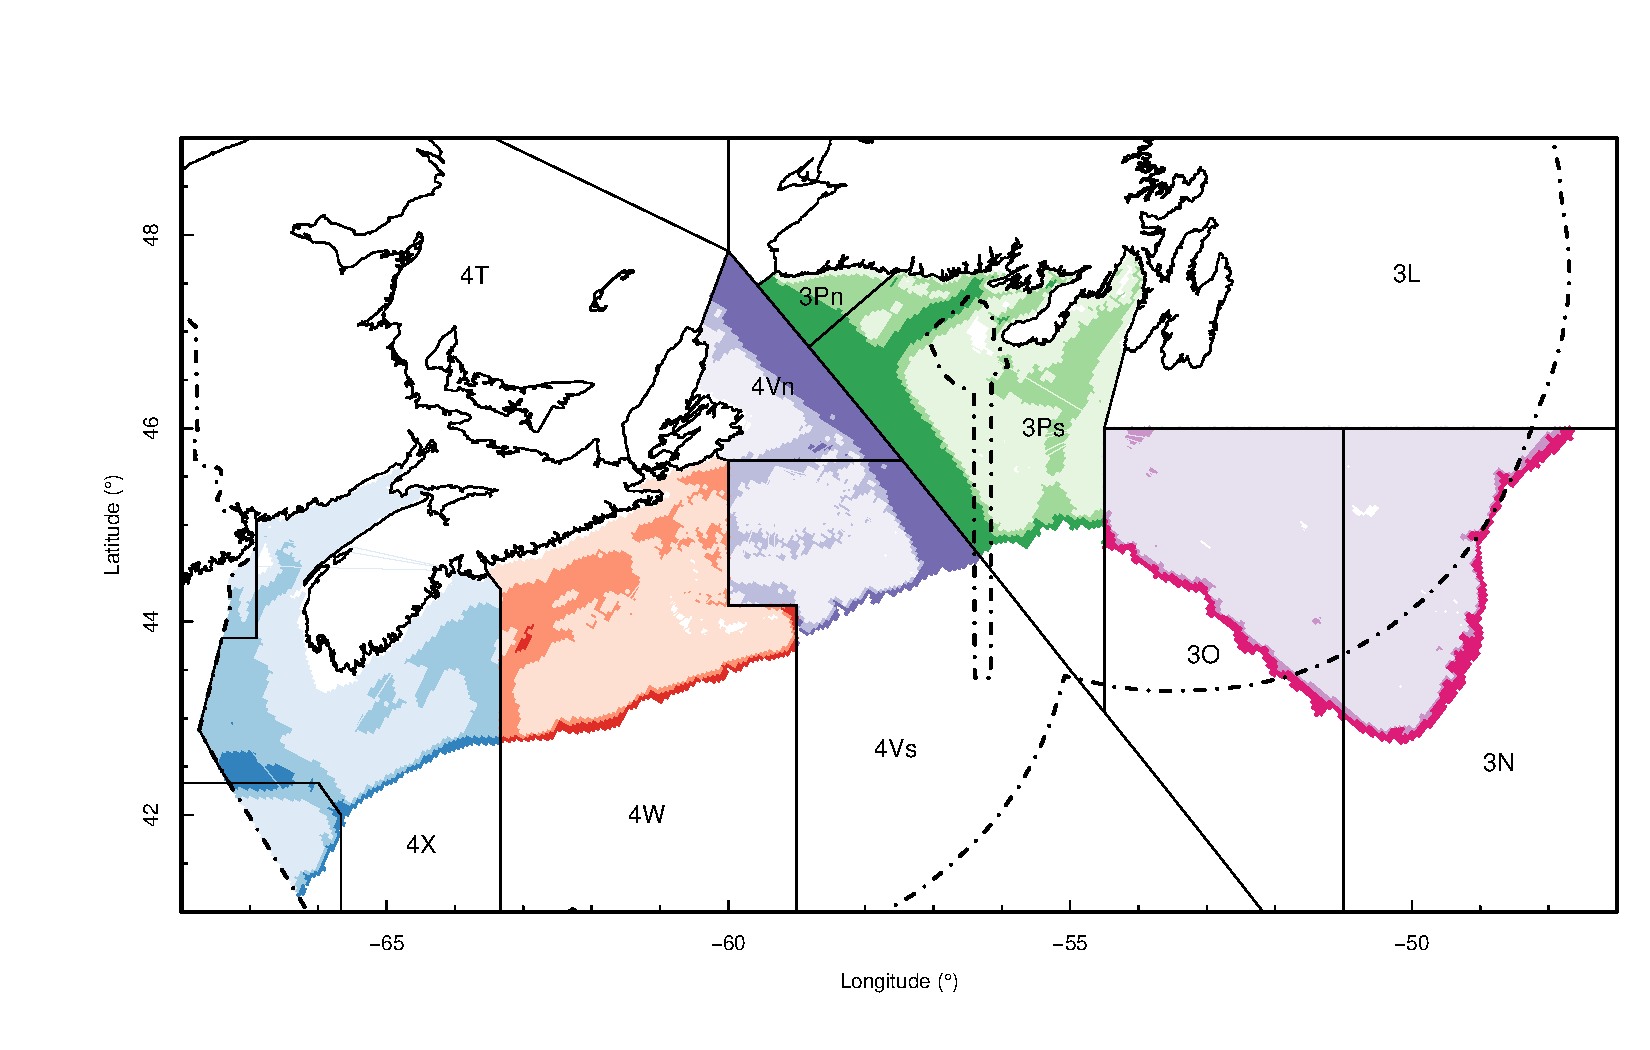
\includegraphics[width=0.75\linewidth]{SurveyStrata}}{Figure \ref{fig:nafo-strat}} 

}

\caption{NAFO divisions on the Scotian Shelf and the Southern Grand Banks. The 3NOPs4VWX5Zc Atlantic halibut stock survey area is denoted by the coloured area, with five area strata: 4X5YX (blues), 4W (oranges), 4V (purples), 3P (greens), and 3NO (reds), and three depth strata: 30 to 130 m (light colour), 131 to 250 m (medium colour), and 251 to 750 m (dark colour). NAFO subdivisions are labelled, and separated by solid lines. The exclusive economic zones of Canada and France are shown with dashed lines. NAFO subdivision 3Pn is not part of the stock area, but is currently included in the survey.}\label{fig:nafo-strat}
\end{figure}
There are 2 Atlantic Halibut management units in Canada. The focus of this work is the Scotian Shelf and Southern Grand Banks management unit which encompasses the North Atlantic Fisheries Organization (NAFO) divisions 3NOPs4VWX5Zc. The other NAFO division 4RST encompasses the Gulf of St.~Lawrence and will not be included in our analysis. The definition of this NAFO division is mostly based on tagging studies that showed Atlantic halibut moving throughout most of the Canadian North Atlantic (DFO \protect\hyperlink{ref-DFO2021}{2021}), which has been supported by recent genetic analysis (Kess et al. \protect\hyperlink{ref-Kess2021}{2021}). Halibut is caught throughout the management unit and on the tail of the Grand Banks outside of Canada's exclusive economic zone (EEZ), mostly along the continental shelf (DFO \protect\hyperlink{ref-DFO2021}{2021}), see Figure~\ref{fig:nafo-strat}.

Due to the nature of spatial modelling and our desire to scale station-specific indices up to an overal index representing the whole area, the area modelled is bounded by the continental shelf (750 m) as shown in Figure~\ref{fig:nafo-strat}. Since no survey ever extends outside of these edges and we do not wish to extrapolate outside the bounds of the observations, restricting our model to this area was determined to be appropriate.

\hypertarget{survey-designs}{%
\subsection{Survey designs}\label{survey-designs}}

As mentioned previously, there are 2 surveys with different sampling designs that are included in this work: a survey that follows a fixed stations design that goes from 1998 to the present day, and a survey following a stratified random sampling design that started in 2017.

\hypertarget{fixed-stations-design}{%
\subsubsection{Fixed Stations Design}\label{fixed-stations-design}}

The formulation of this survey followed a stratified design with fixed stations with the original number of stations set to 222, with 30 reserved for the 3NOPs subdivision (den Heyer et al. \protect\hyperlink{ref-DenHeyer2015}{2015}). The strata were defined based on the observed landings by trips between 1993 and 1997 using 3 categories: high catches (\textgreater250 kg), medium catches (50-249 kg) and low catches (\textless49 kg) with the number of planned stations proportionally allocated following a ratio of 5:7:10 for the low, medium, and high strata respectively (Zwanenburg and Wilson \protect\hyperlink{ref-Zwanenburg2000}{2000}; Zwanenburg et al. \protect\hyperlink{ref-Zwanenburg2003}{2003}; den Heyer et al. \protect\hyperlink{ref-DenHeyer2015}{2015}; Smith \protect\hyperlink{ref-Smith2016a}{2016}). Station coverage has been inconsistent over time as not all stations have been covered every year with new stations being added in the mid-2000s (den Heyer et al. \protect\hyperlink{ref-DenHeyer2015}{2015}). The number of fixed stations decreased to around 100 a year in 2017 and onwards due to the implementation of the new stratified random survey. See Table~\ref{tab:stat-samp} for the number of stations sampled every year.

Survey fishing protocol is 1000 hook sets left in the water for 10 hours and using Mustad circle hooks \#14 or greater between 4 am and noon, but there have been variations in both number and size of hooks (size \#16 hooks becoming more common later in the time series) (den Heyer et al. \protect\hyperlink{ref-DenHeyer2015}{2015}). The start or end of the longline is supposed to be within 3 nautical miles of the station. Vessel and captain participation has varied over time due to many different factors, with 66 different vessels sampling the fixed stations since 2000. \textbf{The number of halibut (including sub-legal size fish) and non-target species are counted in each set.}
\begin{longtable}[]{@{}cccc@{}}
\caption{\label{tab:stat-samp}Number of successfully sampled stations by sampling design between 1998 and 2021.}\tabularnewline
\toprule
Year & Fixed Stations & Stratified Stations & Total Stations\tabularnewline
\midrule
\endfirsthead
\toprule
Year & Fixed Stations & Stratified Stations & Total Stations\tabularnewline
\midrule
\endhead
1998 & 174 & N/A & 174\tabularnewline
1999 & 166 & N/A & 166\tabularnewline
2000 & 216 & N/A & 216\tabularnewline
2001 & 190 & N/A & 190\tabularnewline
2002 & 199 & N/A & 199\tabularnewline
2003 & 188 & N/A & 188\tabularnewline
2004 & 215 & N/A & 215\tabularnewline
2005 & 164 & N/A & 164\tabularnewline
2006 & 163 & N/A & 163\tabularnewline
2007 & 241 & N/A & 241\tabularnewline
2008 & 281 & N/A & 281\tabularnewline
2009 & 205 & N/A & 205\tabularnewline
2010 & 215 & N/A & 215\tabularnewline
2011 & 217 & N/A & 217\tabularnewline
2012 & 217 & N/A & 217\tabularnewline
2013 & 233 & N/A & 233\tabularnewline
2014 & 232 & N/A & 232\tabularnewline
2015 & 232 & N/A & 232\tabularnewline
2016 & 227 & N/A & 227\tabularnewline
2017 & 98 & 141 & 239\tabularnewline
2018 & 100 & 150 & 250\tabularnewline
2019 & 98 & 123 & 221\tabularnewline
2020 & 99 & 148 & 247\tabularnewline
2021 & 98 & 131 & 229\tabularnewline
\bottomrule
\end{longtable}
\hypertarget{stratified-random-design}{%
\subsubsection{Stratified Random Design}\label{stratified-random-design}}

The sampling design for this survey follows a stratified random sampling design, where the strata are the 5 NAFO subdivisions (4X5YZ, 4W, 4V, 3P, 3NO) each with 3 depth strata (30-130 m, 131-250 m, 251-750 m) and includes 3Pn and some area outside of Canada's EEZ, which are not part of the management unit (Cox et al. \protect\hyperlink{ref-Cox2018}{2018}; Luo et al. \protect\hyperlink{ref-Luo2022}{2022}). The depth bounds (30-750 m) were chosen as they contain most of the survey sets, most of the Atlantic halibut habitat, and were based on exploratory analyses of catch rates by depth from the fixed stations (Cox et al. \protect\hyperlink{ref-Cox2018}{2018}). Around 150 survey stations a year are randomly assigned to strata with the number in a given stratum proportional to its size (Cox et al. \protect\hyperlink{ref-Cox2018}{2018}; Luo et al. \protect\hyperlink{ref-Luo2022}{2022}). The fishing protocol is similar to the fixed stations protocol but notably more strictly defined, with each set containing 1000 baited hooks with size \#15 hooks set for between 6 and 12 hours (Luo et al. \protect\hyperlink{ref-Luo2022}{2022}). 40 different vessels have participated in the stratified survey sampling design, with 19 of those also sampling some of the fixed stations at some point (meaning 21 vessels have only participated in this survey design).

Unlike the fixed stations, the observers collecting the stratified random survey data must also record hook condition data on a subset of hooks for each set. Based on a pilot study that aimed to calculate the size required to be broadly representative of the whole set (Doherty et al. \protect\hyperlink{ref-Doherty2017}{2017}), 10 samples of 30 hooks across the line are chosen for this increased data collection for a total of 300 per 1000 hooks (Luo et al. \protect\hyperlink{ref-Luo2022}{2022}). Instead of simply counting the number of halibut \textbf{(including sub-legal size fish)} and non-target species caught, the condition of each hook (baited, unbaited, broken, missing) is also recorded for this subsample. See Table~\ref{tab:stat-samp} for the number of stations sampled every year.

\hypertarget{model-formulation}{%
\subsection{Model Formulation}\label{model-formulation}}

\hypertarget{mem}{%
\subsubsection{MEM}\label{mem}}

The original aim of the MEM was to account for hook competition in longline fishing as proposed by Rothschild (\protect\hyperlink{ref-Rothschild1967}{1967}) and reformulated by Etienne et al. (\protect\hyperlink{ref-Etienne2013}{2013}). There are two different formulations of the MEM, which will respectively be called the Full MEM and the Reduced MEM.

The Reduced MEM allows for three possible outcomes for every hook following the summation \(N_i = N_{B,i}+N_{T,i}+N_{NT,i}\), wherein the total number of hooks \(N_i\) on a longline set \(i\) is the sum of the number of hooks with non-target species \(N_{NT,i}\), the number of hooks with target species \(N_{T,i}\), and the number of hooks without any animals that are assumed to still be baited \(N_{B,i}\). Assuming that the time to catch a target or non-target species follows independent exponential distributions with rates \(\lambda_T\) and \(\lambda_{NT}\), then the the vector \((N_{B,i},N_{T,i},N_{NT,i})\) follows a multinomial distribution (Etienne et al. \protect\hyperlink{ref-Etienne2013}{2013}; Luo \protect\hyperlink{ref-Luo2020}{2020}; Luo et al. \protect\hyperlink{ref-Luo2022}{2022}):
\begin{equation}
(N_{B,i},N_{T,i},N_{NT,i}) \sim \mathcal{M}(N_i,\alpha_i) \ \ where
\end{equation} \begin{equation}
\alpha_i = (e^{-\lambda S_i},(1-e^{-\lambda S_i})\frac{\lambda_T}{\lambda},(1-e^{-\lambda S_i})\frac{\lambda_{NT}}{\lambda}),
\end{equation}
\(S_i\) is the soak time of longline set \(i\), and \(\lambda = \lambda_T + \lambda_{NT}\).

This formulation does not account for the condition of hooks that return without catching animals, as these are not guaranteed to still be baited. Etienne et al. (\protect\hyperlink{ref-Etienne2013}{2013}) therefore reformulated this MEM into the Full MEM, wherein hooks can also come back unbaited (which includes broken or missing hooks). These empty hooks are assumed to come from interactions with animals, but due to identifiability concerns another assumption has to be made as to whether they are caused by target or non-target species (Etienne et al. \protect\hyperlink{ref-Etienne2013}{2013}). Since the gear is more likely to be oriented towards catching target species and that non-target species are likely more abundant (encompassing many more species than just the main target), it seemed more reasonable to assume that empty or broken hooks were caused by non-target species (Etienne et al. \protect\hyperlink{ref-Etienne2013}{2013} p. @Luo2022). This extra outcome is therefore added to the multinomial model, which now follows the following distribution:
\begin{equation}
(N_{B,i},N_{T,i},N_{NT,i},N_{E,i}) \sim \mathcal{M}(N_i,\alpha_i) \ \ where
\end{equation} \begin{equation}
\alpha_i = (e^{-\lambda S_i},(1-e^{-\lambda S_i})\frac{\lambda_T}{\lambda},(1-e^{-\lambda S_i})\frac{\lambda_{NT}}{\lambda}(1-p_{NT}),(1-e^{-\lambda S_i})\frac{\lambda_{NT}p_{NT}}{\lambda}),
\end{equation}
\(N_{E,i}\) is the number of empty hooks, and \(p_{NT}\) is the probability of escape of non-target animals. In this formulation, \(p_{NT}\) shows up in the calculation of \(N_{NT,i}\), as it impacts the catch rates of non-target species. As this component is present in the Reduced MEM and those non-target species would be similarly able to escape as in the Full MEM, we modified the Reduced MEM so that the multinomial component \(N_{NT,i}\) is obtained as \((1-e^{-\lambda S_i})\frac{\lambda_{NT}}{\lambda}(1-p_{NT})\). While it is unlikely that this version of the Reduced MEM can reliably estimate \(p_{NT}\), it should be able to borrow the information from the Full MEM when both datasets are analyzed in the same framework.

\hypertarget{memspa}{%
\subsubsection{MEMSpa}\label{memspa}}

While the MEM model achieved its goal of incorporating hook competition to improve estimates of catch rates, it did not account for spatial patterns in the survey data. Previous work (Luo \protect\hyperlink{ref-Luo2020}{2020}; Luo et al. \protect\hyperlink{ref-Luo2022}{2022}) harnessed geostatistical approaches to modify both versions of the MEM through the use of Gaussian Random Fields (GRF).

The observation level of this new MEMSpa remained almost the same as described in the previous section, but the rates \(\lambda_T\) and \(\lambda_{NT}\) were modified to incorporate the location of a given longline set \(i\):
\begin{equation}
\lambda_{T,i} = exp(\beta_T+\omega_{T,i})
\end{equation} \begin{equation}
\lambda_{NT,i} = exp(\beta_{NT}+\omega_{NT,i})
\end{equation}
where \(\lambda_{T,i}\) and \(\lambda_{NT,i}\) are the exponential rates for target and non-target species at the location of longline set \(i\), \(\beta_T\) and \(\beta_{NT}\) are intercept parameters, and \(\omega_{T,i}\) and \(\omega_{NT,i}\) are the values of the underlying GRF.

These modifications allow the model to incorporate spatial patterns present in the data to obtain station-specific catch rates.An additional requirement is to be able to obtain a single overall estimated rate for the entire modelled area to be treated as an index of relative abundance. Due to the computational load of utilizing kriging to obtain this index, a Dirichlet method is preferred wherein the modelled area is divided into disjoint tiles based on the survey station locations, and each station is associated with a specific region and assumed to be representative of it (Luo et al. \protect\hyperlink{ref-Luo2022}{2022}). One can then obtain a spatially-weighted survey index for the whole area:
\begin{equation}
Overall Index = \frac{\sum_{i=1}^I A_i \hat{\lambda}_i}{\sum_{i=1}^I A_i}
\end{equation}
where \(A_i\) is the area of the Dirichlet tile associated with station \(i\), \(\hat{\lambda}_i\) is the corresponding estimated catch rate at this station, and \(I\) is the total number of stations.

As the data from the stratified random survey only has a subset of its hooks where the hook condition was recorded, a product likelihood approach was taken so as to incorporate all the available data inside a unified framework. This consists of separately fitting the Reduced MEMSpa to the data without hook condition and the Full MEMSpa to the data with hook condition, and multiplying their likelihoods together (see Luo et al. (\protect\hyperlink{ref-Luo2022}{2022}) for more details on MEMSpa).

\hypertarget{spatio-temporal-mem}{%
\subsubsection{Spatio-Temporal MEM}\label{spatio-temporal-mem}}

The improvements brought forward by the inclusion of spatial patterns in MEMSpa were very clear when fitted to the stratified dataset, but there still remained 20 years of available information from the fixed stations. Furthermore, the spatial model could only be fitted to a single year at a time and hence did not account for any temporal patterns in halibut or non-target species distributions and abundance. Incorporating these patterns into MEMSpa would result in a fully spatio-temporal MEM.

As we aim to retain the inclusion of spatial patterns through the residual structure as done in MEMSpa, the temporal aspects would need to be incorporated (following the regression framework of MEMSpa) in the mean structure instead. There are many different approaches to the incorporation of temporal patterns in the mean for fisheries models which usually involve random effects, with common approaches including random intercepts (Venables and Dichmont \protect\hyperlink{ref-Venables2004}{2004}; Kai et al. \protect\hyperlink{ref-Kai2017}{2017}; Pedersen et al. \protect\hyperlink{ref-Pedersen2018}{2018}), random slopes (Venables and Dichmont \protect\hyperlink{ref-Venables2004}{2004}; Swain et al. \protect\hyperlink{ref-Swain2009}{2009}), random walks (Swain et al. \protect\hyperlink{ref-Swain2009}{2009}; Li et al. \protect\hyperlink{ref-Li2019}{2019}), or autoregressive models (Schnute and Richards \protect\hyperlink{ref-Schnute1995}{1995}; Kai et al. \protect\hyperlink{ref-Kai2017}{2017}). These last two could also be seen as more structured versions of other approaches wherein the random walk or autoregressive structure would be on the random intercept. Furthermore, we also decided to control for the impact of different survey vessels through random vessel effects. The novel formulation takes the following form:
\begin{equation}\label{eq:rand-int}
\lambda_{T,i,y} = exp(\eta_{T,y}+ \nu_{T,j}+\omega_{T,i,y})
\end{equation} \begin{equation}\label{eq:rand-slope}
\lambda_{T,i,y} = exp(\beta_T+\eta_{T,y}+ \nu_{T,j}+\omega_{T,i,y})
\end{equation}
where \(\nu_{T,j}\) is the mean 0 normally distributed random effect of vessel \(j\) with associated variance \(\sigma_\nu^2\), \(\eta_{T,y}\) are the random intercepts for target species in year \(t\) or, in Equation~\ref{eq:rand-slope}, the random slopes in year \(t\) with global intercept \(\beta_T\). In Equation~\ref{eq:rand-int}, \(\eta_{T,y} \sim N(\mu_{T,int},\sigma_{T,int}^2)\), while for Equation~\ref{eq:rand-slope} \(\mu_{T,int}=0\). For the random walk and autoregressive models, they follow the same formulation as Equation~\ref{eq:rand-int} with the following added structure on \(\eta_{T,y}\):
\begin{equation}\label{eq:rand-walk}
\eta_{T,y} = \eta_{T,y-1} + \epsilon_y, \ \ \ \epsilon_y ~ N(0,\sigma_\eta^2)
\end{equation} \begin{equation}\label{eq:ar1}
\eta_{T,y} = c + \phi \eta_{T,y-1} + \epsilon_y, \ \ \ \epsilon_y ~ N(0,\sigma_\eta^2)
\end{equation}
where \(\epsilon_y\) is a 0 mean normally distributed error term with variance \(\sigma_\eta^2\). The autoregressive model in Equation~\ref{eq:ar1} is a first order autoregressive (AR(1)) process with constant mean \(c\) and autoregressive parameter \(\phi\) bounded between -1 and 1 to ensure stationarity. Non-target rates would follow the same structure with non-target specific parameters. Importantly, this formulation allows us to incorporate fixed and random effects for target and non-target vessels for both target and non-target species separately, as the catch rates for both would not necessarily be impacted the same way by a given fishing vessel.

These models are fit to the data from both surveys. As the fixed stations data do not contain any information on hook condition, only the Reduced MEM can be fit to it. Model validation will be done by comparing root mean squared errors (RMSE), and by calculating AIC and BIC values for the 4 different model fits. There are 2 types of errors to look at in this model, one being the GRF at the hierarchical level of the catch rates \(\lambda\) and the other being the difference between the observations and the expected observations based on the probabilities obtained from the multinomial distribution. Either way, the RMSE is calculated as:
\begin{equation}
RMSE = \frac{\sum_{i=1}^N e_i^2}{N}
\end{equation}
where \(e_i\) is the error, either the GRF value \(\omega_{i,y}\) for rate \(i\) in year \(y\) or the sum difference between observed number of target, non-target and hooks and the expected number of each respective values for a given longline set \(i\).

AIC (Akaike \protect\hyperlink{ref-Akaike1974}{1974}) and BIC (Schwarz \protect\hyperlink{ref-Schwarz1978}{1978}) are both information criterion that are used to compare different model fits that try to balance between better model fit (through higher likelihood) and number of parameters. They are respectively calculated as:
\begin{equation}\label{eq:aic}
AIC = 2K - 2 log(L)
\end{equation} \begin{equation}\label{eq:bic}
BIC = K log(n) - 2 log(L)
\end{equation}
where \(K\) is the number of parameters, \(log(\cdot)\) is the natural log, \(L\) is the maximized likelihood, and \(n\) is the number of data points.

\hypertarget{data}{%
\subsection{Data}\label{data}}

Once the best model is chosen, the model will be applied to various subsets of the data to be able to compare and better understand the model output. These different data subsets are: the stratified data (2017 to 2020), the fixed stations (1998 to 2020), both datasets in years where both are available (2017 to 2020) and both datasets for all years (1998 to 2020). \textbf{To compare to current approaches, the mean observed catch rate in each year is also calculated by dividing the observed number of halibuts caught at each station by the product of the number of hooks and the soak time of each station to ensure that we are comparing methods on the same scale. This is done separately for both datasets combined and for the fixed station dataset.}

\hypertarget{persistence-of-spatial-patterns}{%
\subsection{Persistence of spatial patterns}\label{persistence-of-spatial-patterns}}

While this was not required by the terms of reference, a quick analysis of the ability of the fixed stations data to accurately capture changes over time of Atlantic halibut and non-target species abundance was undertaken, mainly due to the fact that obtaining an unbiased estimate of population abundance when only using fixed stations is very difficult due to the absence of reliable design-based estimators (Li et al. \protect\hyperlink{ref-Li2015}{2015}; Lee and Rock \protect\hyperlink{ref-Lee2018}{2018}). Furthermore, an underlying assumption behind this type of design is that the spatial distribution of the population of interest is consistent over time (Li et al. \protect\hyperlink{ref-Li2015}{2015}; Lee and Rock \protect\hyperlink{ref-Lee2018}{2018}). In our case, this means that the distribution of Atlantic halibut and non-target species would have to be consistent with their spatial distribution between 1995 and 1997 as the strata were defined by the distribution of catches in 1995-1997. The fixed station design was able to detect changes in abundance (den Heyer et al. \protect\hyperlink{ref-DenHeyer2015}{2015}; Trzcinski and Bowen \protect\hyperlink{ref-Trzcinski2016}{2016}; Li et al. \protect\hyperlink{ref-Li2022}{2022}), but there was concern that catch rates might not be proportional to abundance (Smith \protect\hyperlink{ref-Smith2016a}{2016}; Cox et al. \protect\hyperlink{ref-Cox2018}{2018}). As this stock recovered, the distribution of the commercial fishery changed and expanded (den Heyer et al. \protect\hyperlink{ref-DenHeyer2015}{2015}; Li et al. \protect\hyperlink{ref-Li2022}{2022}), highlighting the need for survey coverage throughout the management unit.

A relatively straightforward approach to test the fixed stations for their ability to appropriately track population abundance change over time is test the persistence of these distributions over time (Lee and Rock \protect\hyperlink{ref-Lee2018}{2018}). As our data, even when transformed from counts to catch rates, violated the basic assumptions of the traditional ANOVA approach chosen by Lee and Rock (\protect\hyperlink{ref-Lee2018}{2018}), we instead decided to take the more simple approach of doing pairwise comparisons between years of Atlantic halibut catch rates and non-target species catch rates, which can be calculated as follow (Warren \protect\hyperlink{ref-Warren1994}{1994}; Li et al. \protect\hyperlink{ref-Li2015}{2015}):
\begin{equation}
\bar{\omega} = \frac{s^2_y/4}{s^2_s-s^2_y/4}
\end{equation}
where \(\bar{\omega}\) is the measurement of persistence degree wherein a smaller value indicates a greater degree of persistence, \(s^2_y\) is the difference in catch rates of the same site between compared years, and \(s^2_s\) is the difference in catch rates between different sites in the same year. These last 2 variables are calculated as:
\begin{equation}
s^2_s = \frac{\sum_{y=1}^2 \sum_{y=1}^{n_i} (x_{iy}-\bar{x}_y)^2}{m_1+m_2-2}
\end{equation} \begin{equation}
s^2_y = \sum_{i=1}^m (d_i - \bar{d})^2 / (m-1)
\end{equation}
where \(x_{iy}\) is the observed catch rate in site \(i\) and year \(y\), \(\bar{x}_y\) is the mean observed catch rate of year \(y\), \(m_1\) is the number of fixed stations in the first year included in the pairwise comparison while \(m_2\) is the same for the second year, \(d_i\) is the different in catch rate between two years in site \(i\) and \(\bar{d}\) is the mean catch rate difference. An important note here is that, as the coverage of stations changed over time, there are often more stations included in the \(s^2_s\) than \(s^2_y\) as all stations in both years are included in \(s^2_s\), but only the stations fished in both years can be included in \(s^2_y\).

\hypertarget{results}{%
\section{Results}\label{results}}

\hypertarget{model-validation}{%
\subsection{Model Validation}\label{model-validation}}

Out of the 4 models that were fit to the data, 3 of them (random intercept, random walk and AR(1) process) successfully converged but the model with random slopes resulted in false convergence and was therefore rejected. The RMSE, AIC and BIC values from this model validation process can be seen in Table~\ref{tab:valid}. These values appear to indicate that there is very little difference between the model fits as the RMSE are almost all identical to the \(5^{th}\) decimal. According to the AIC and BIC values, the best model would be the random walk as it has the lowest values for both metrics, although the difference is not very large. The model used for all analysis moving forward is therefore the random walk model.

\begingroup\fontsize{9}{11}\selectfont
\begingroup\fontsize{9}{11}\selectfont
\begin{longtable}[t]{cccccc}
\caption{\label{tab:valid}Outputs for model validation approaches, including root mean squared errors (RMSE), Akaike Information Criterion (AIC) and Bayesian Information Criterion (BIC).}\\
\toprule
\textbf{Model} & \textbf{Observation RMSE} & \textbf{Target Field RMSE} & \textbf{Non-Target Field RMSE} & \textbf{AIC} & \textbf{BIC}\\
\midrule
\endfirsthead
\caption*{}\\
\toprule
\textbf{Model} & \textbf{Observation RMSE} & \textbf{Target Field RMSE} & \textbf{Non-Target Field RMSE} & \textbf{AIC} & \textbf{BIC}\\
\midrule
\endhead

\endfoot
\bottomrule
\endlastfoot
Random Intercept & 0.6711538 & 1.311270 & 1.705561 & 230,733.0 & 230,817.3\\
Random Walk & 0.6711406 & 1.301307 & 1.711642 & 230,673.6 & 230,757.9\\
AR(1) Process & 0.6711534 & 1.311766 & 1.705651 & 230,735.6 & 230,832.8\\*
\end{longtable}
\endgroup{}
\endgroup{}

\hypertarget{fit-to-data}{%
\subsection{Fit to Data}\label{fit-to-data}}

As the best model was considered to be the random walk approach, that model was the one fit to the varying data subsets. Due to issues fitting the 1999 data to the spatial model and to various versions of a spatio-temporal model, the analysis focuses on the data starting in 2000 and does not incorporate the data from 1998 and 1999.

The model successfully converged for all cases, but the fits with the 2017 and onwards data show signs of overparameterization as all of them have at least 1 variance parameter related to the random intercepts that is estimated arbitrarily close to 0 (see Table~\ref{tab:par-estim}). Most other parameters are estimated very similarly for all fits with the exception of \(p_{nt}\) and \(\mu_{nt}\). \(p_{nt}\) is estimated at a very low value when only the fixed stations are included with a correspondingly lower estimate of \(\mu_{nt}\), while fits that include the stratified data estimate both parameters at significantly higher values.

\begingroup\fontsize{7}{9}\selectfont
\begingroup\fontsize{7}{9}\selectfont
\begin{longtable}[t]{cccccc}
\caption{\label{tab:par-estim}Estimated values of parameter for each different model fit with standard error in parentheses.}\\
\toprule
\textbf{Parameter} & \textbf{Both Datasets (Full)} & \textbf{Fixed Stations (Full)} & \textbf{Both Datasets (2017+)} & \textbf{Fixed Station (2017+)} & \textbf{Stratified Data (2017+)}\\
\midrule
\endfirsthead
\caption*{}\\
\toprule
\textbf{Parameter} & \textbf{Both Datasets (Full)} & \textbf{Fixed Stations (Full)} & \textbf{Both Datasets (2017+)} & \textbf{Fixed Station (2017+)} & \textbf{Stratified Data (2017+)}\\
\midrule
\endhead

\endfoot
\bottomrule
\endlastfoot
$p_{nt}$ & 0.788 (0.001) & 0.129 (0.009) & 0.881 (0.0005) & 0.246 (0.015) & 0.903 (0.0005)\\
Anisotropy Parameter 1 & -0.100 (0.027) & -0.081 (0.026) & -0.131 (0.095) & -0.186 (0.079) & -0.085 (0.090)\\
Anisotropy Parameter 2 & -0.021 (0.025) & 0.020 (0.026) & -0.019 (0.066) & 0.129 (0.077) & -0.147 (0.078)\\
$\phi_t$ & 0.050 (0.002) & 0.053 (0.002) & 0.054 (0.005) & 0.060 (0.007) & 0.058 (0.007)\\
$\phi_{nt}$ & 0.048 (0.001) & 0.060 (0.002) & 0.015 (0.002) & 0.046 (0.005) & 0.051 (0.005)\\
$\sigma_t$ & 1.619 (0.032) & 1.468 (0.032) & 1.956 (0.085) & 1.408 (0.080) & 1.985 (0.101)\\
$\sigma_{nt}$ & 1.915 (0.030) & 1.599 (0.029) & 1.493 (0.038) & 1.582 (0.074) & 0.885 (0.029)\\
$\sigma_{vess,t}$ & 0.760 (0.099) & 0.601 (0.083) & 0.735 (0.228) & 0.485 (0.174) & 0.505 (0.214)\\
$\sigma_{vess,nt}$ & 0.882 (0.091) & 0.744 (0.088) & 0.746 (0.108) & 0.748 (0.187) & 0.624 (0.092)\\
$\sigma_{int,t}$ & 0.114 (0.038) & 0.185 (0.048) & 0.0003 (0.043) & 0.00010 (0.083) & 0.00005 (0.030)\\
$\sigma_{int,nt}$ & 0.293 (0.074) & 0.078 (0.058) & 0.158 (0.119) & 0.233 (0.220) & 0.0002 (0.038)\\
$\mu_{t}$ & -12.590 (0.221) & -12.866 (0.264) & -12.012 (0.181) & -11.133 (0.174) & -12.262 (0.164)\\
$\mu_{nt}$ & -7.531 (0.384) & -9.432 (0.202) & -6.319 (0.225) & -9.559 (0.381) & -6.015 (0.117)\\*
\end{longtable}
\endgroup{}
\endgroup{}

The distribution of vessel effects are very similar between model fits, with more variability and a wider distribution when more data is incorporated (i.e., fits with just the fixed stations or just the stratified data from 2017 onwards tend to have lower variance and tighter distribution, see Figure~\ref{fig:vess-eff}). This is likely caused by the stricter protocol for the stratified random sets that result in less variability between vessels.
\begin{figure}[htb]

{\centering \pdftooltip{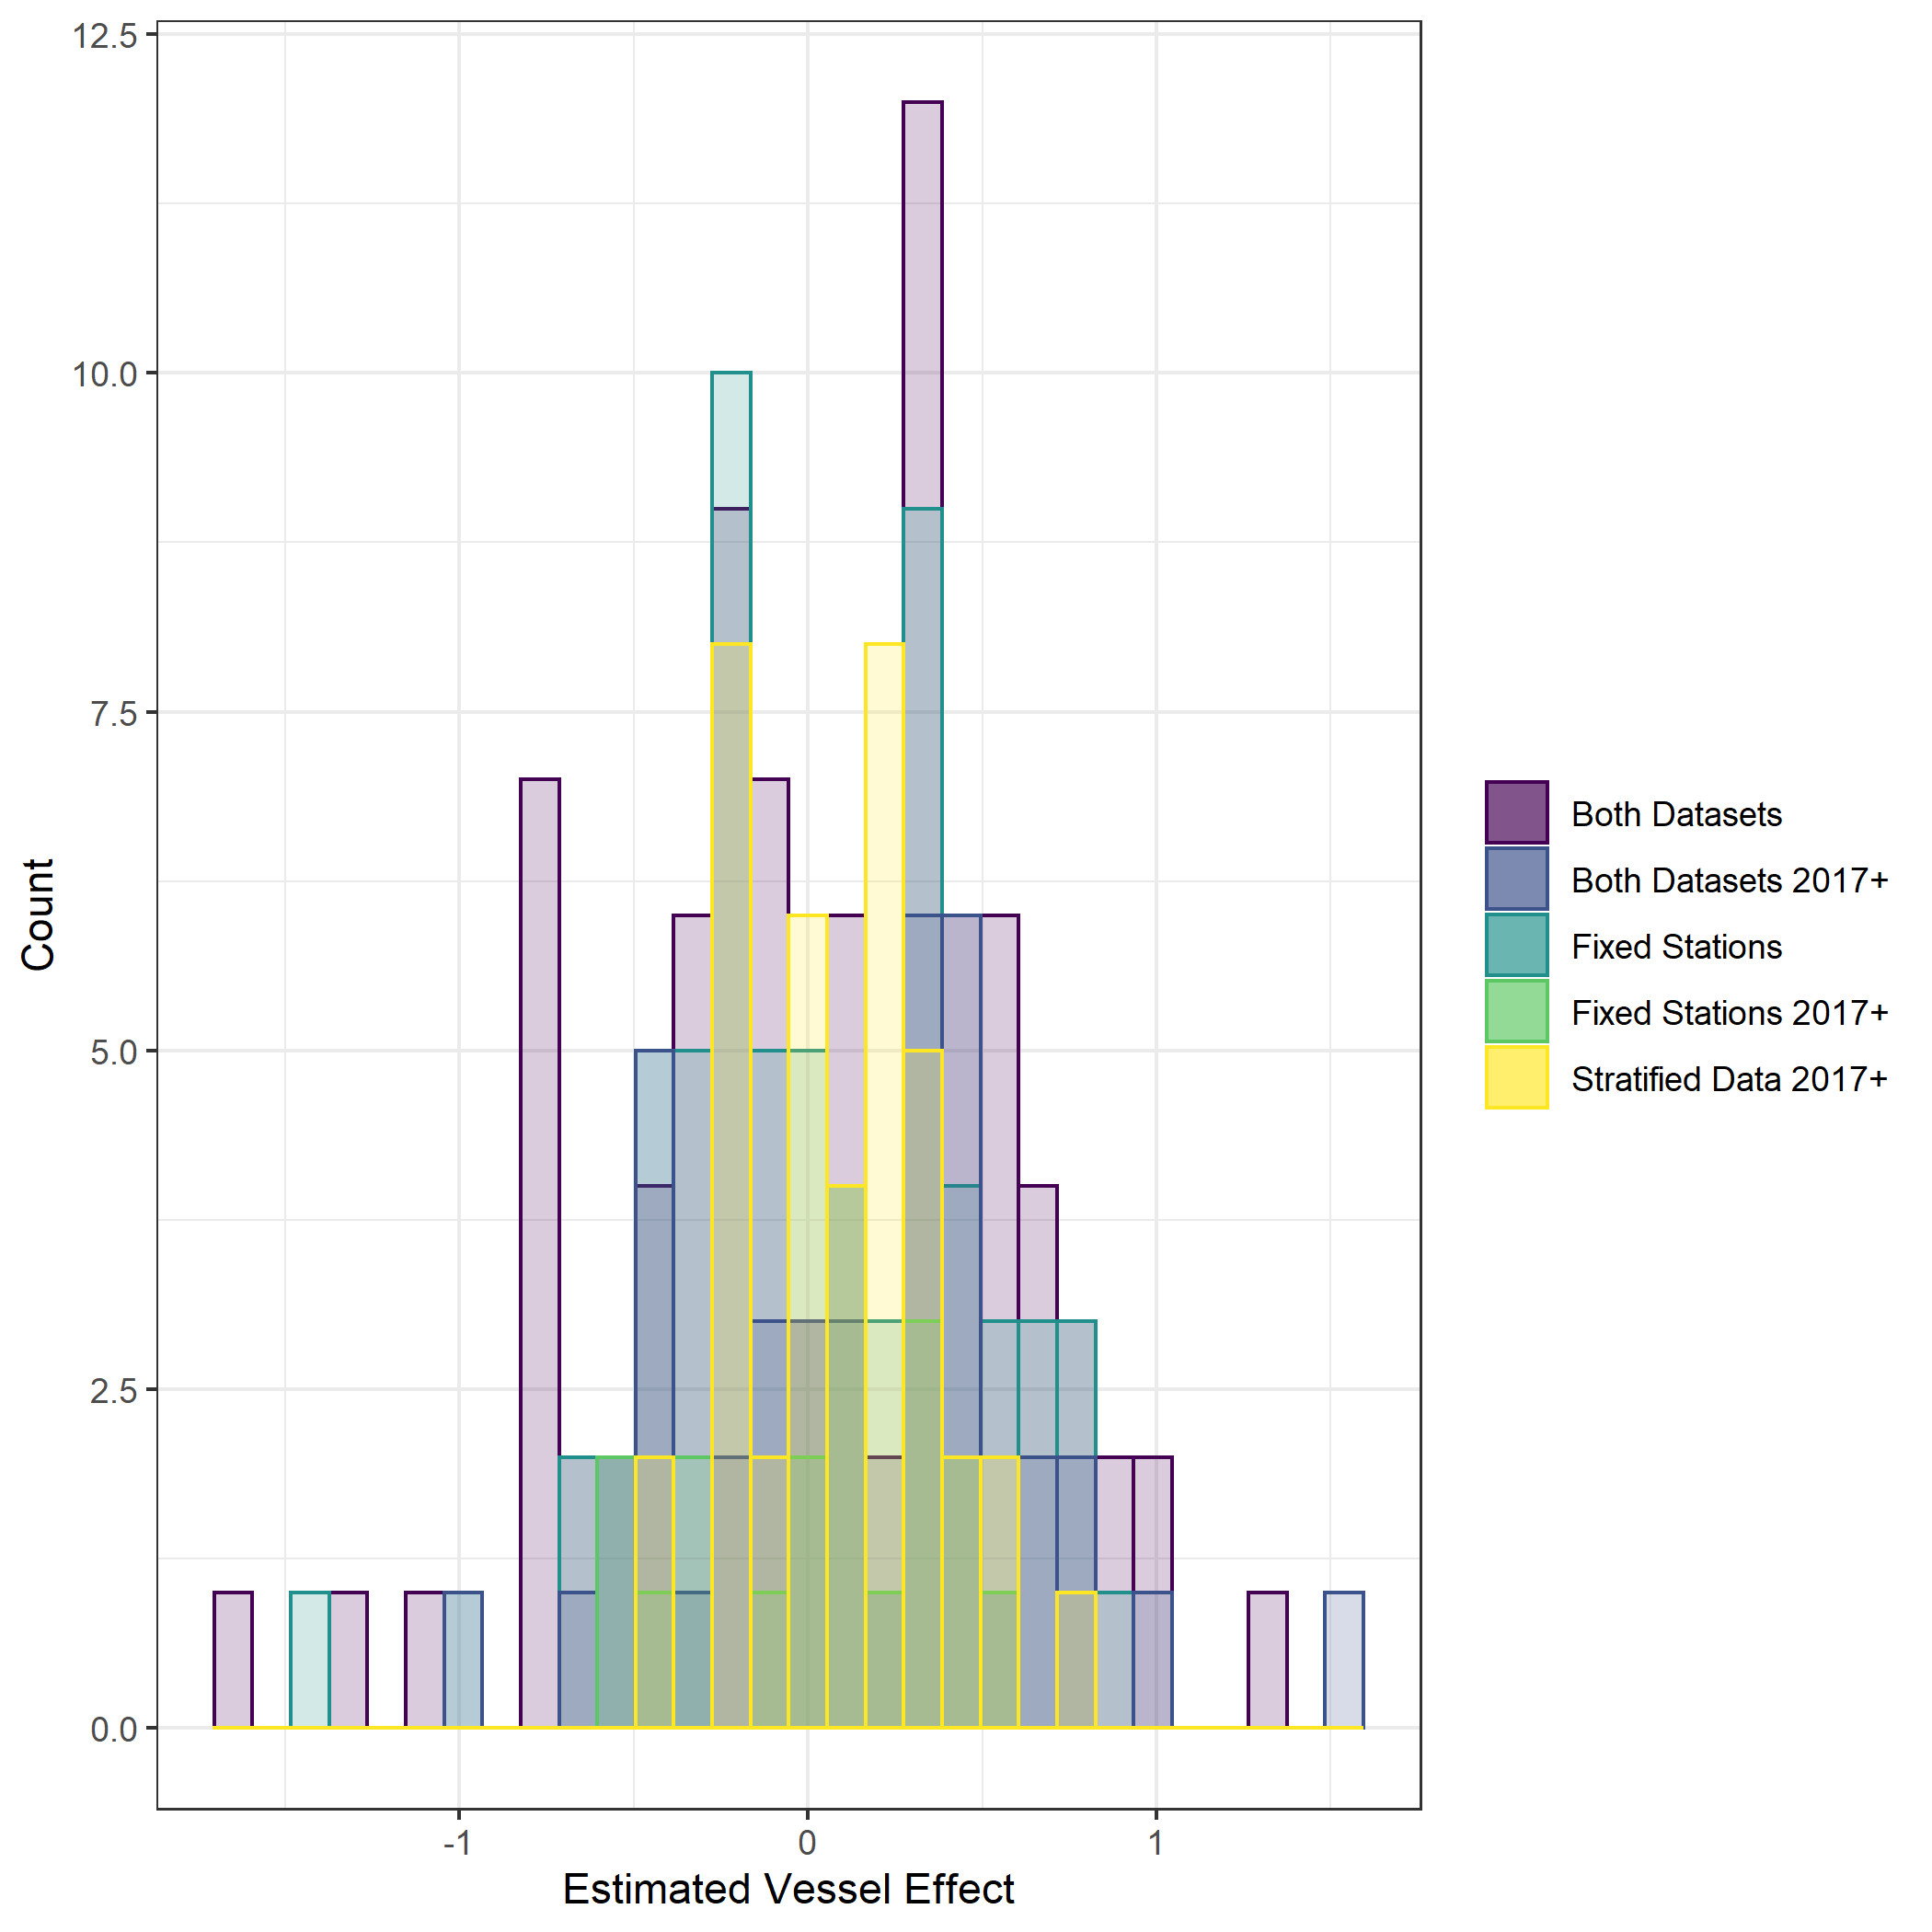
\includegraphics[width=0.6\linewidth]{vess_eff_t_walk}}{Figure \ref{fig:vess-eff}} \pdftooltip{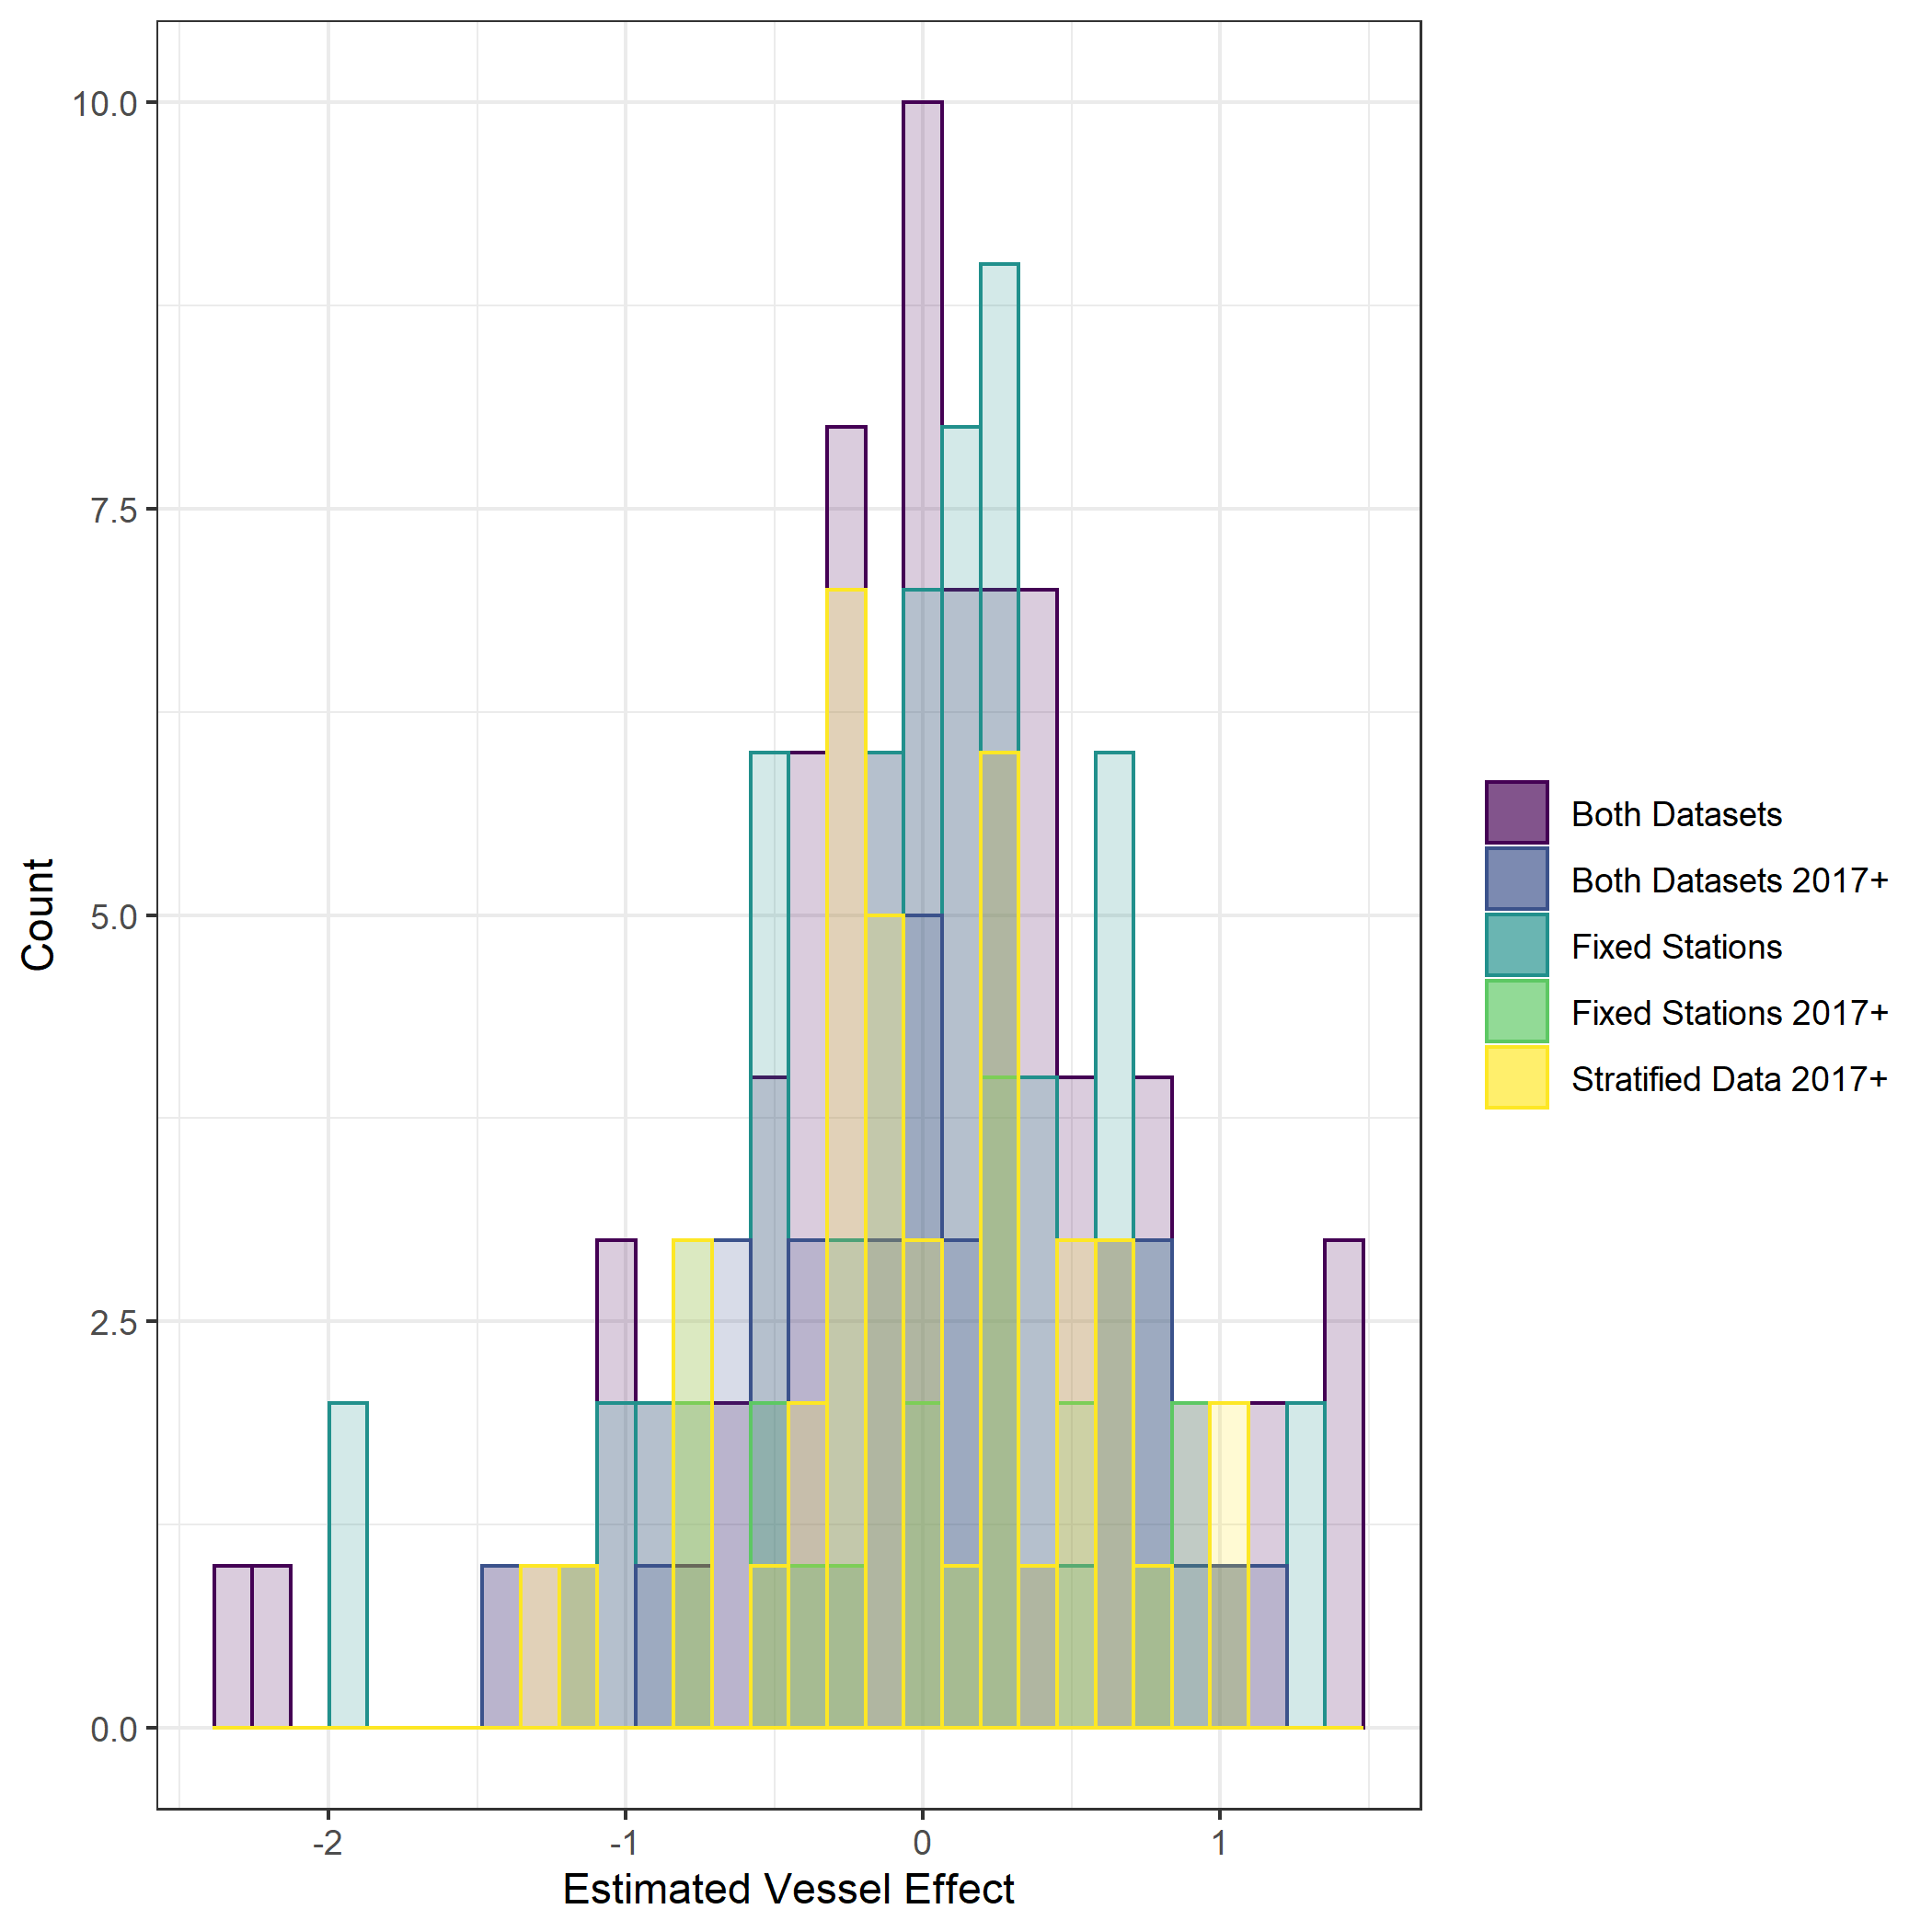
\includegraphics[width=0.6\linewidth]{vess_eff_nt_walk}}{Figure \ref{fig:vess-eff}} 

}

\caption{Distribution of estimated vessel effect using data from the fixed stations and stratified survey design both together and separately between 2000 and 2021 and between 2017 and 2021.}\label{fig:vess-eff}
\end{figure}
The overparameterization of fits that only contain data from 2017 onwards is very visible in Figure~\ref{fig:rand-int} where most intercepts do not vary over time due to the model not being able to estimate the variance around them. For the fits that have data starting in 2000, there are clear changes over time in the random intercepts. Non-target species intercepts are always lower when only the fixed stations are considered, as expected with the difference in the estimated value of \(p_{nt}\). Notably, the stratified random survey, with the additional hook condition data, suggests an increase in overall average expected non-target catch rates starting in 2016 which does not show up when the model is fit only to fixed station data.

The pattern for the target species (halibut) are a lot more similar between model fits, with both capturing an overall increase in expected catch rates over the time series. However, the fit with just the fixed stations has a slightly larger increase.
\begin{figure}[htb]

{\centering \pdftooltip{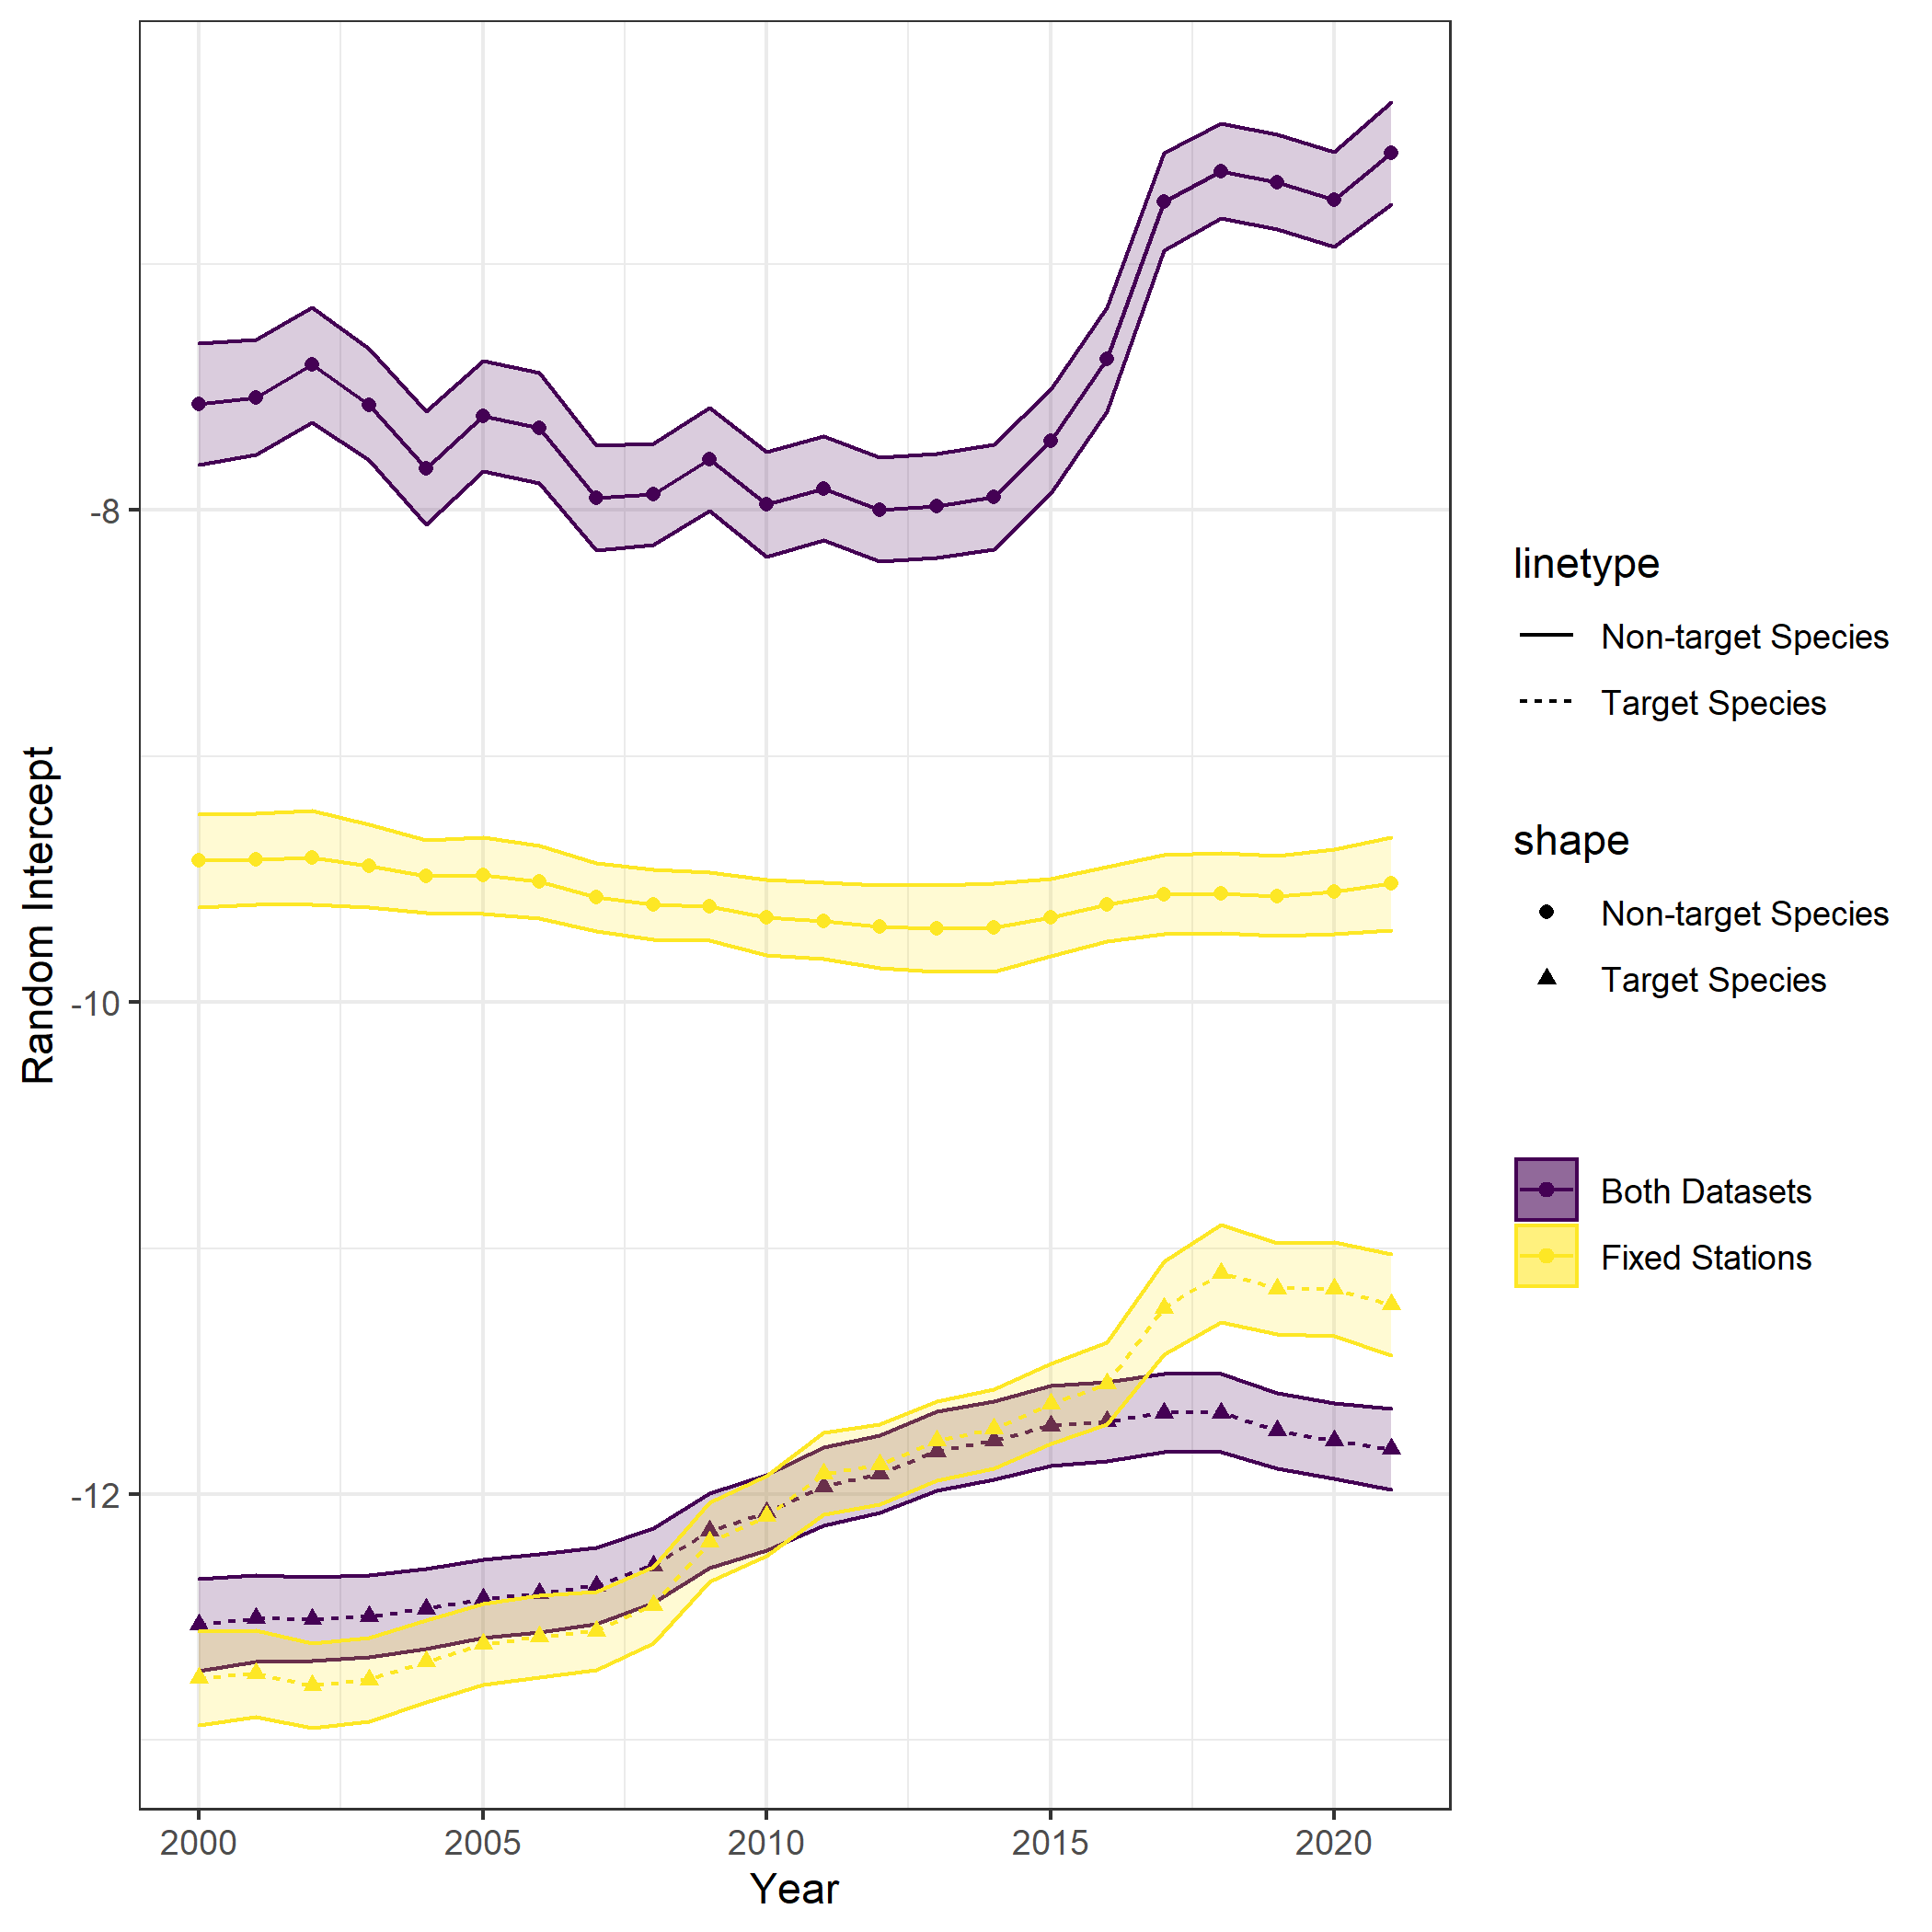
\includegraphics[width=0.6\linewidth]{rand_int_walk}}{Figure \ref{fig:rand-int}} \pdftooltip{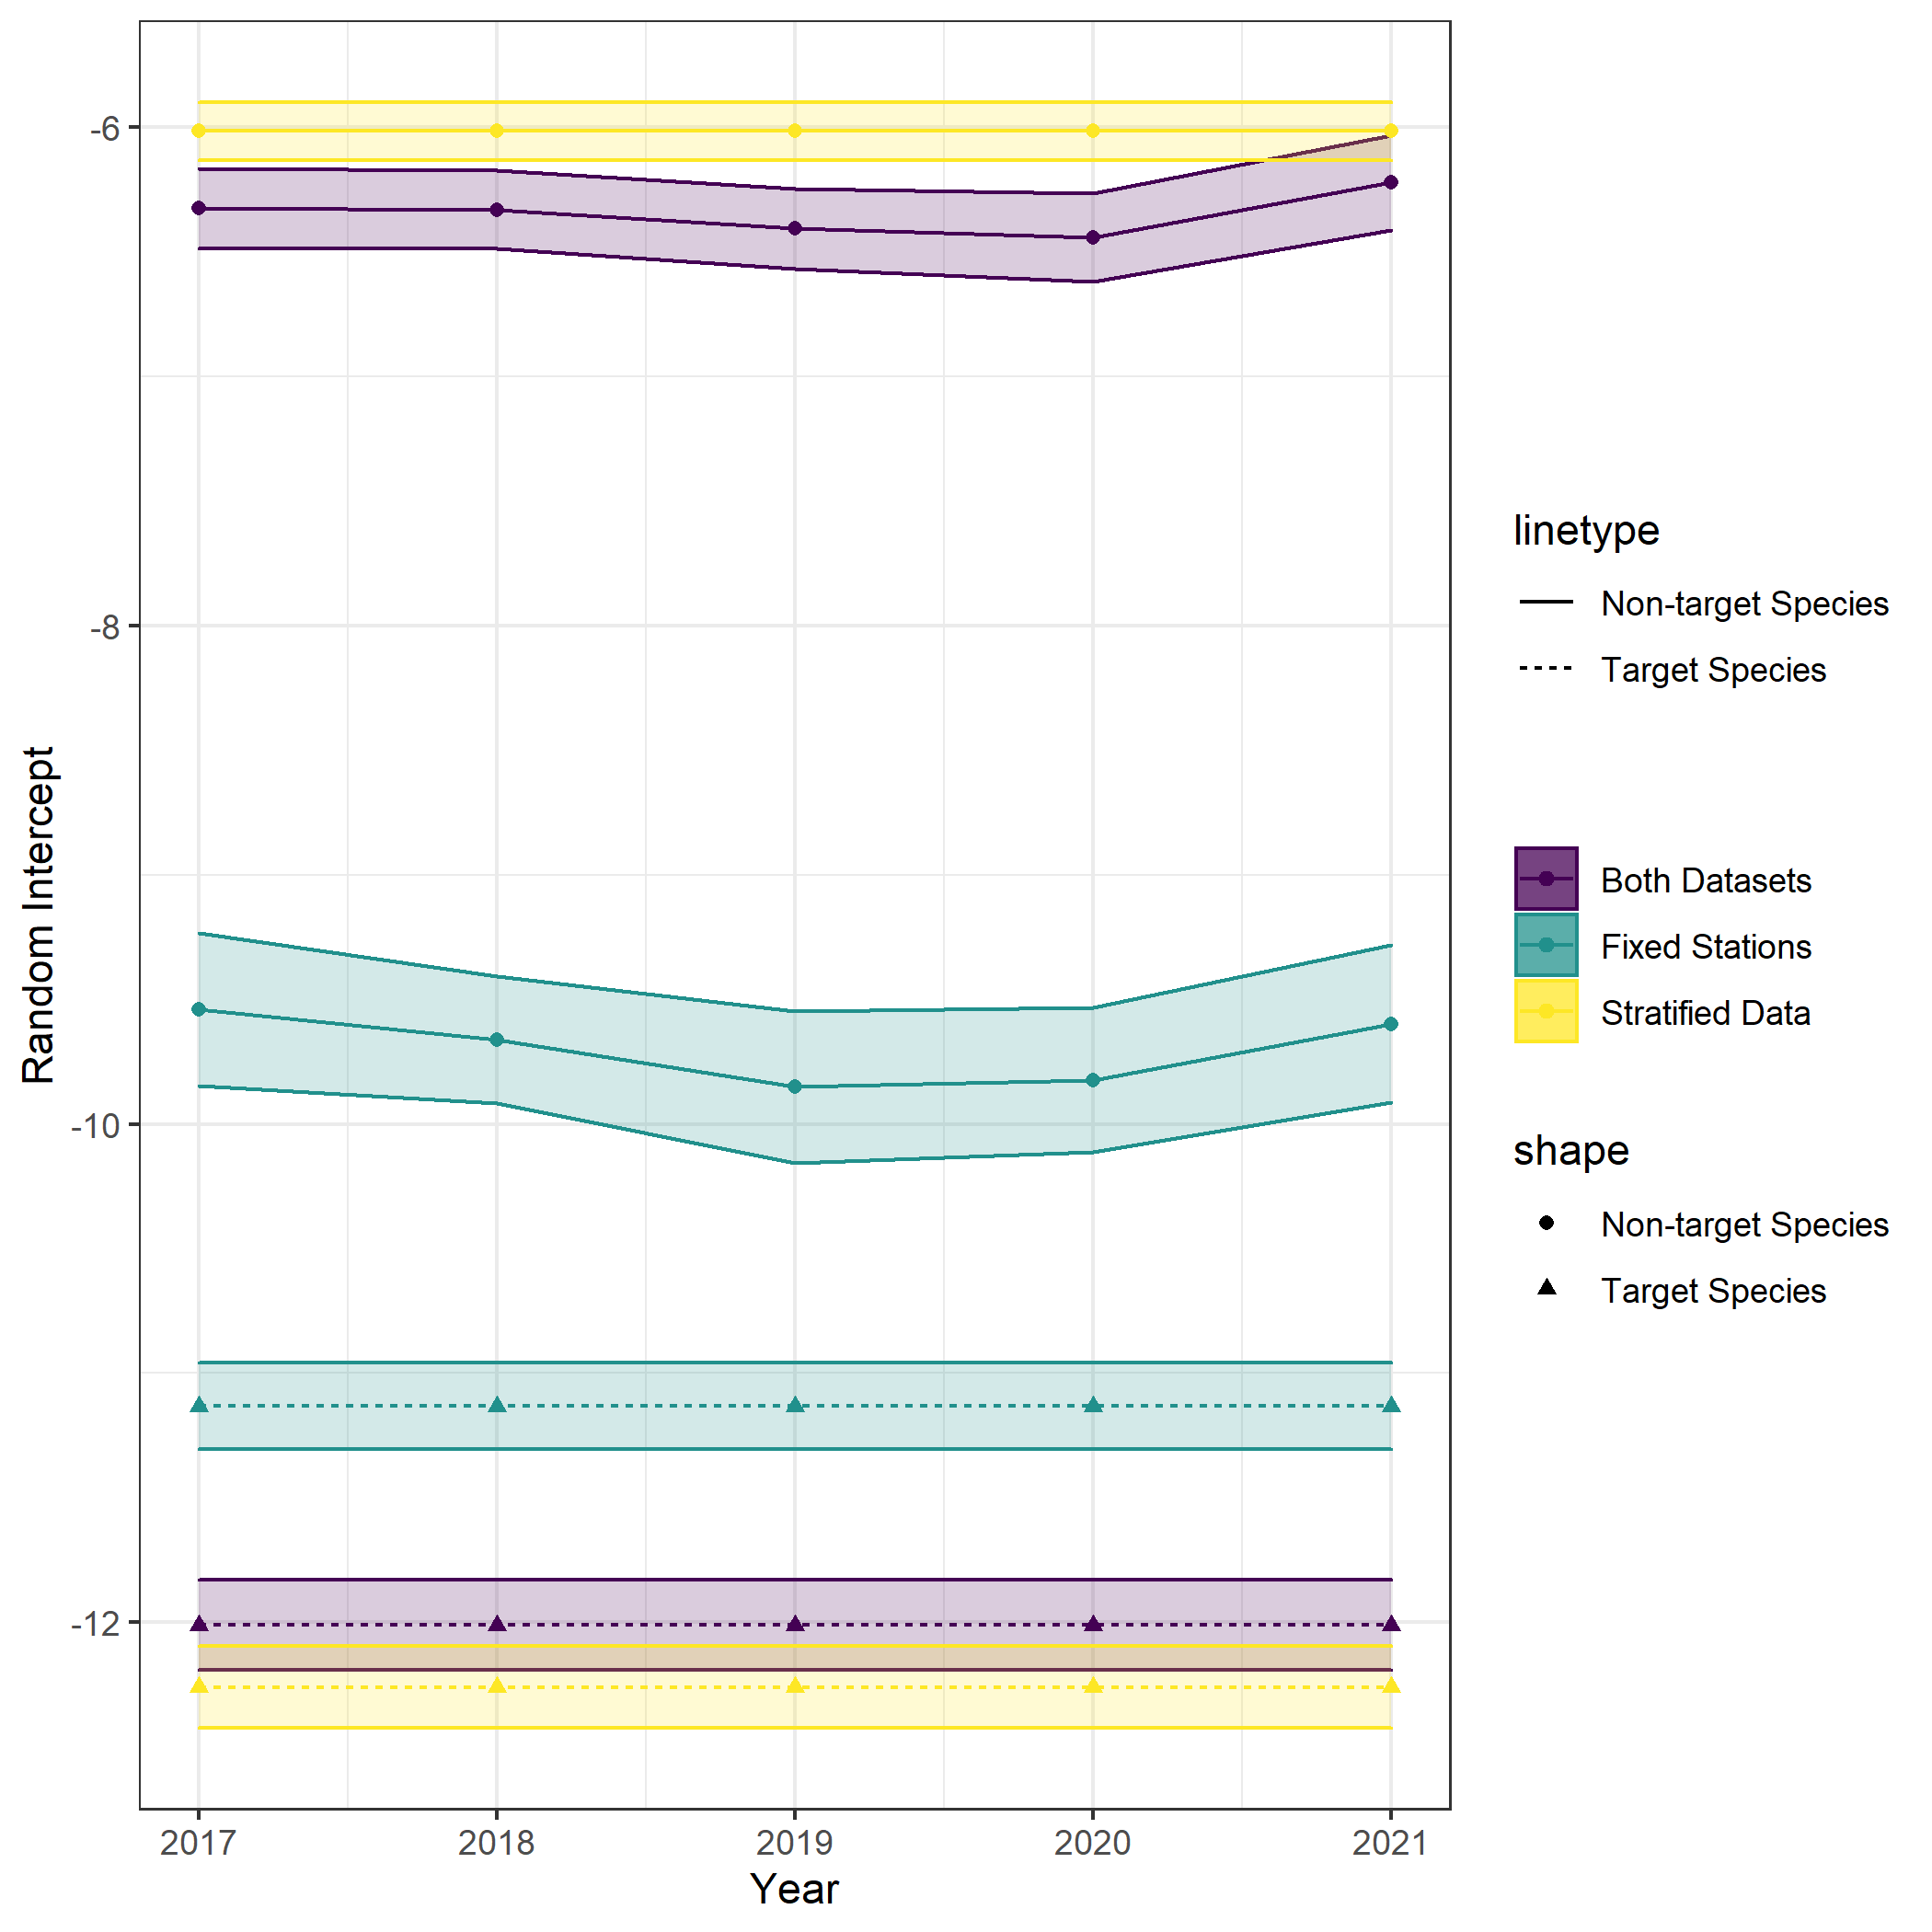
\includegraphics[width=0.6\linewidth]{rand_int_2017_walk}}{Figure \ref{fig:rand-int}} 

}

\caption{Estimated random intercepts using data from the fixed stations and stratified survey design both together and separately between 2000 and 2021 and between 2017 and 2021.}\label{fig:rand-int}
\end{figure}
For the indices themselves (\(\lambda_t\) and \(\lambda_{nt}\)), there are large differences when looking at the fits that only include data from 2017 onwards (Figure~\ref{fig:target-indices}). The fit with just the fixed stations has a completely different pattern than the other 2 fits. Those other 2 fits have similar trends, but the estimates when both datasets are included are more than twice as large as when just the stratified data is included. However, as all these fits are from a model that is overparameterized for the length of time present in the data, it is difficult to find clear links between the datasets and the modelling output.

For the fits that incorporate data starting in 2000, the trends between the two fits are very similar but the fit with both datasets always has larger indices than the one with just fixed stations. Notably, the model estimates a low \(p_{nt}\) for the fixed stations, which implies that the abundance of non-target species is much larger than the number caught and results in lower capture rates (\(\lambda_{nt}\), Figure~\ref{fig:non-t-indices}). \textbf{The one year where trends appear to differ between the two is in 2015, where the fit with both datasets has a spike noticeably absent from the fit with just the fixed stations. This is mostly caused by a couple tows that, due to the difference in \(p_{nt}\), have a noticeably higher estimated halibut catch rate. Since these are located on the eastern edge of the area (see Figure~\ref{fig:target-spat}), they end up being being weighted heavily due to our spatially weighted average approach, which results in the spike in that given year.}
\begin{figure}[htb]

{\centering \pdftooltip{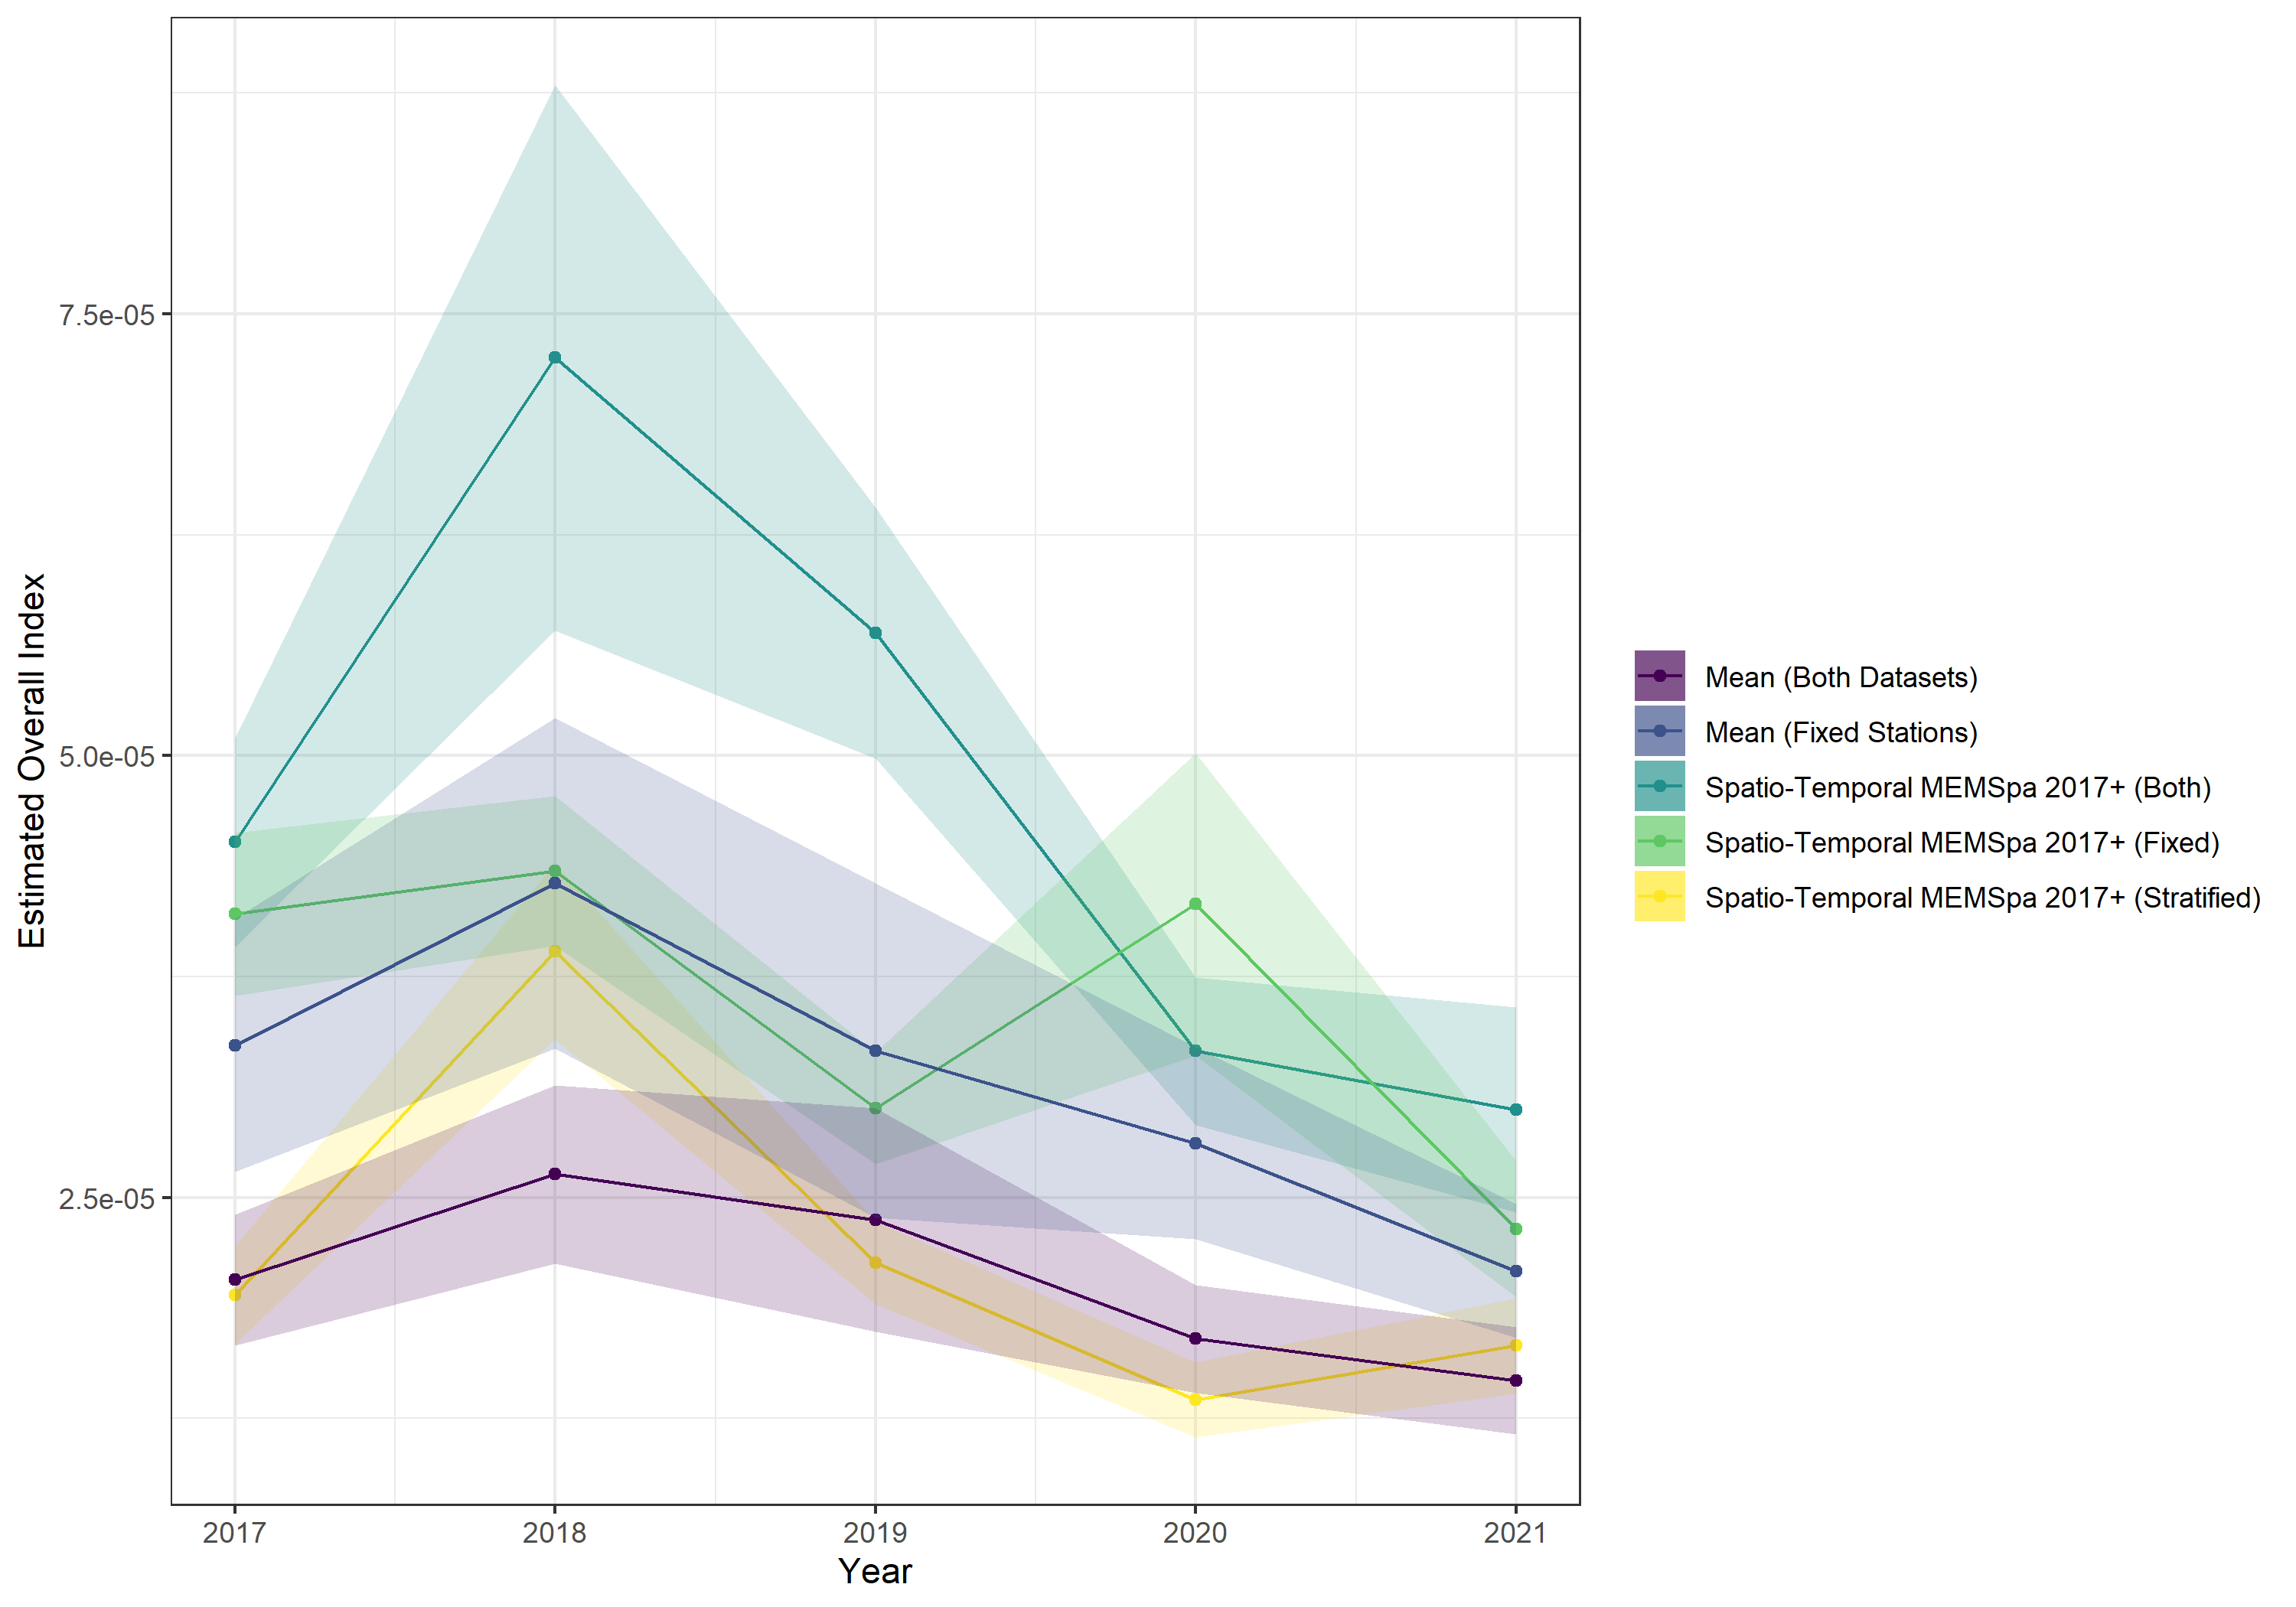
\includegraphics[width=0.75\linewidth]{comp_all_ldat_2017_walk_ver2}}{Figure \ref{fig:target-indices}} \pdftooltip{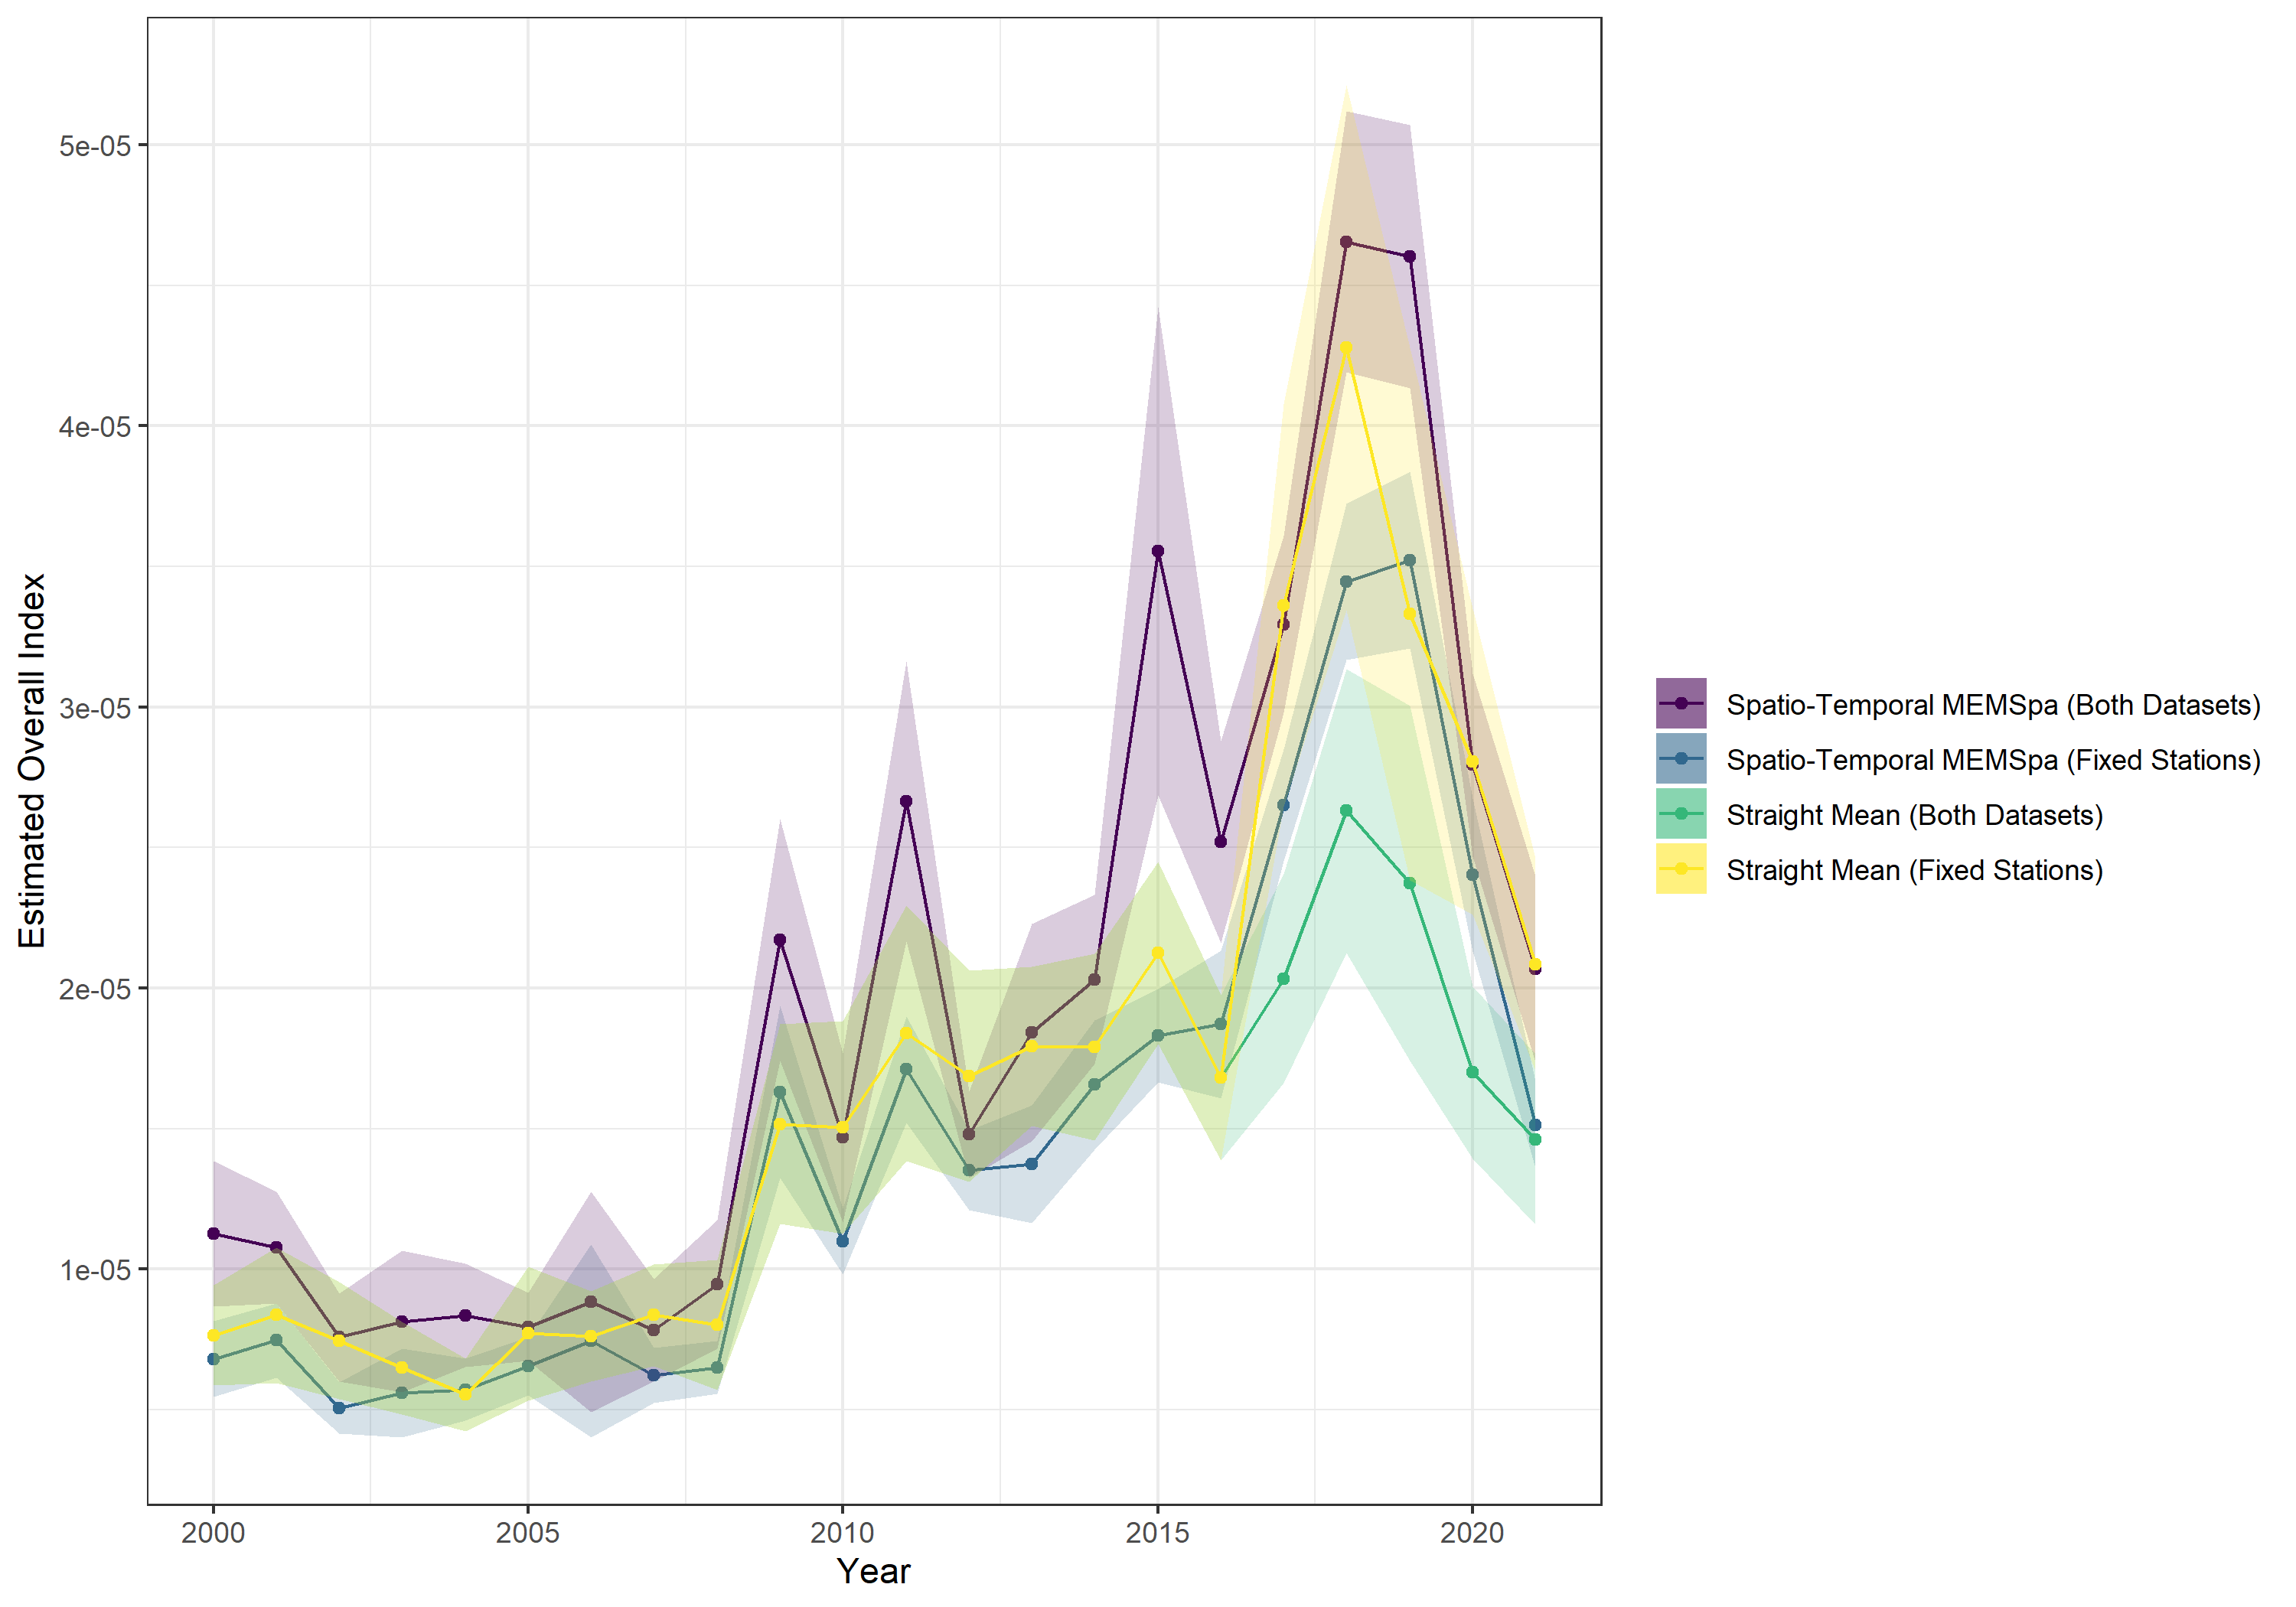
\includegraphics[width=0.75\linewidth]{comp_all_ldat_walk_ver2}}{Figure \ref{fig:target-indices}} 

}

\caption{Estimated overall index for target species using data from the fixed stations and stratified survey design both together and separately, and the mean observed catch rate between 2000 and 2021 and between 2017 and 2021. The uncertainty represent +/- 1 standard error.}\label{fig:target-indices}
\end{figure}
\begin{figure}[htb]

{\centering \pdftooltip{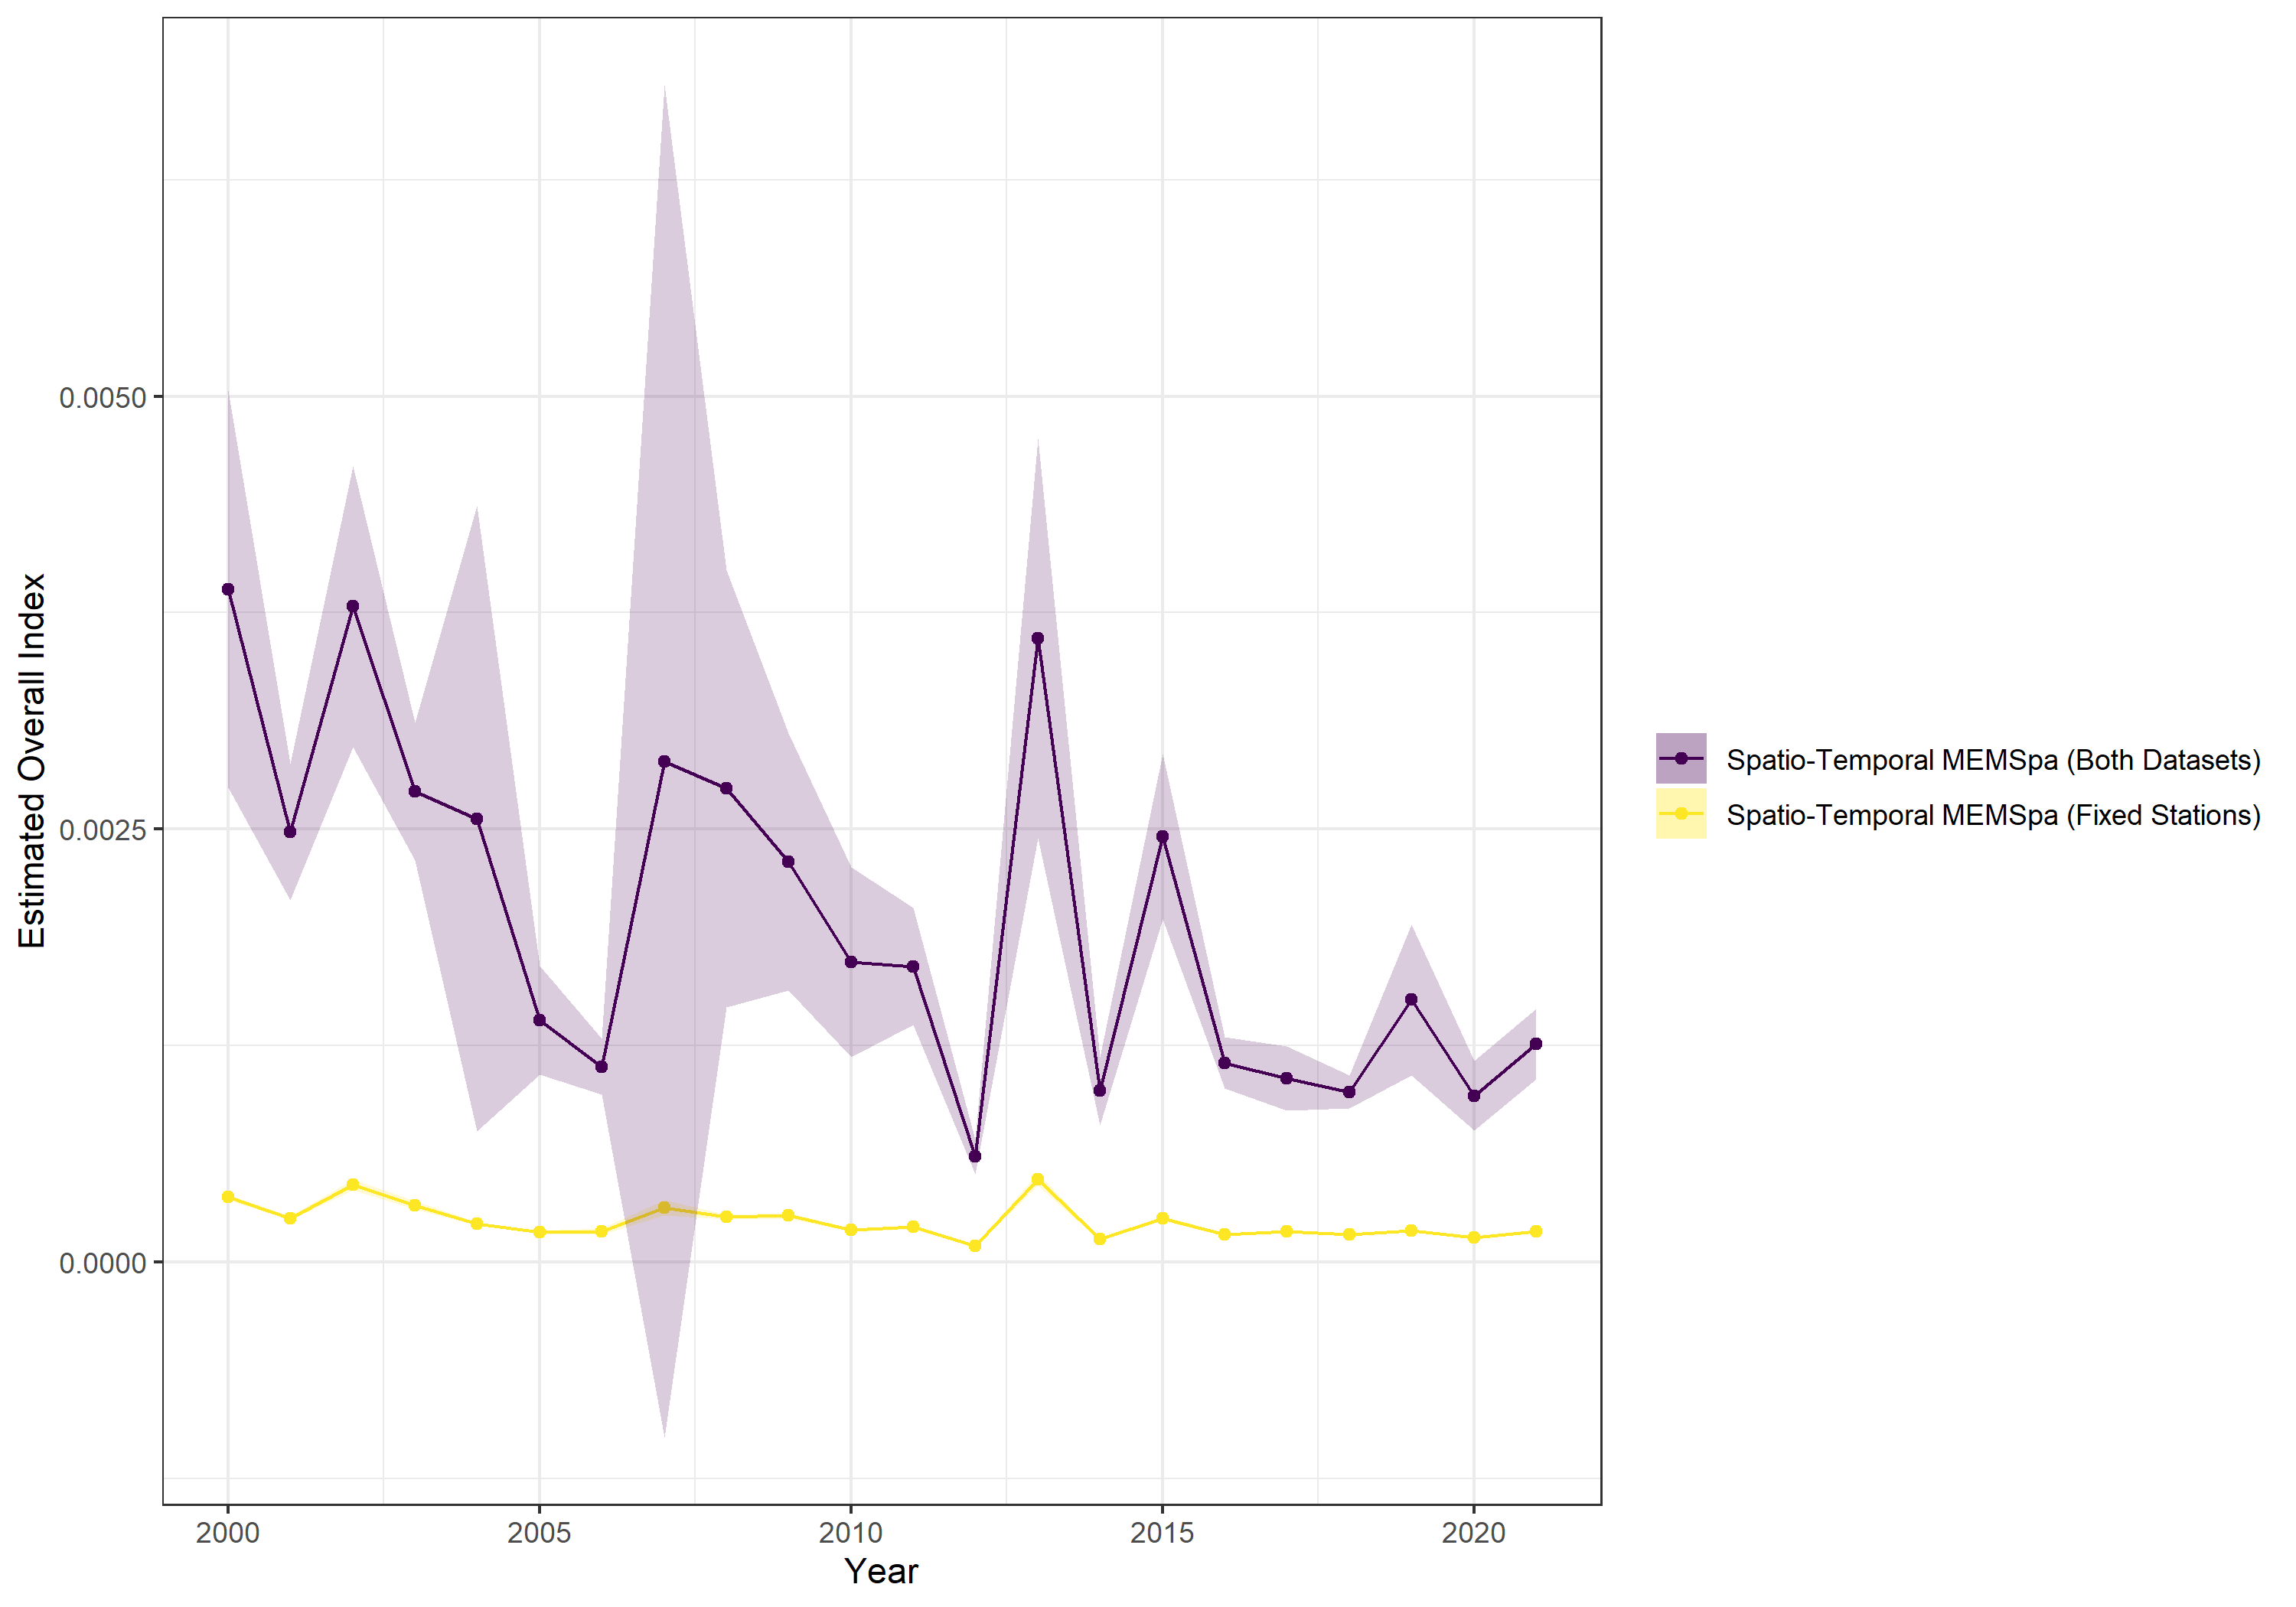
\includegraphics[width=0.75\linewidth]{comp_all_ldant_walk}}{Figure \ref{fig:non-t-indices}} \pdftooltip{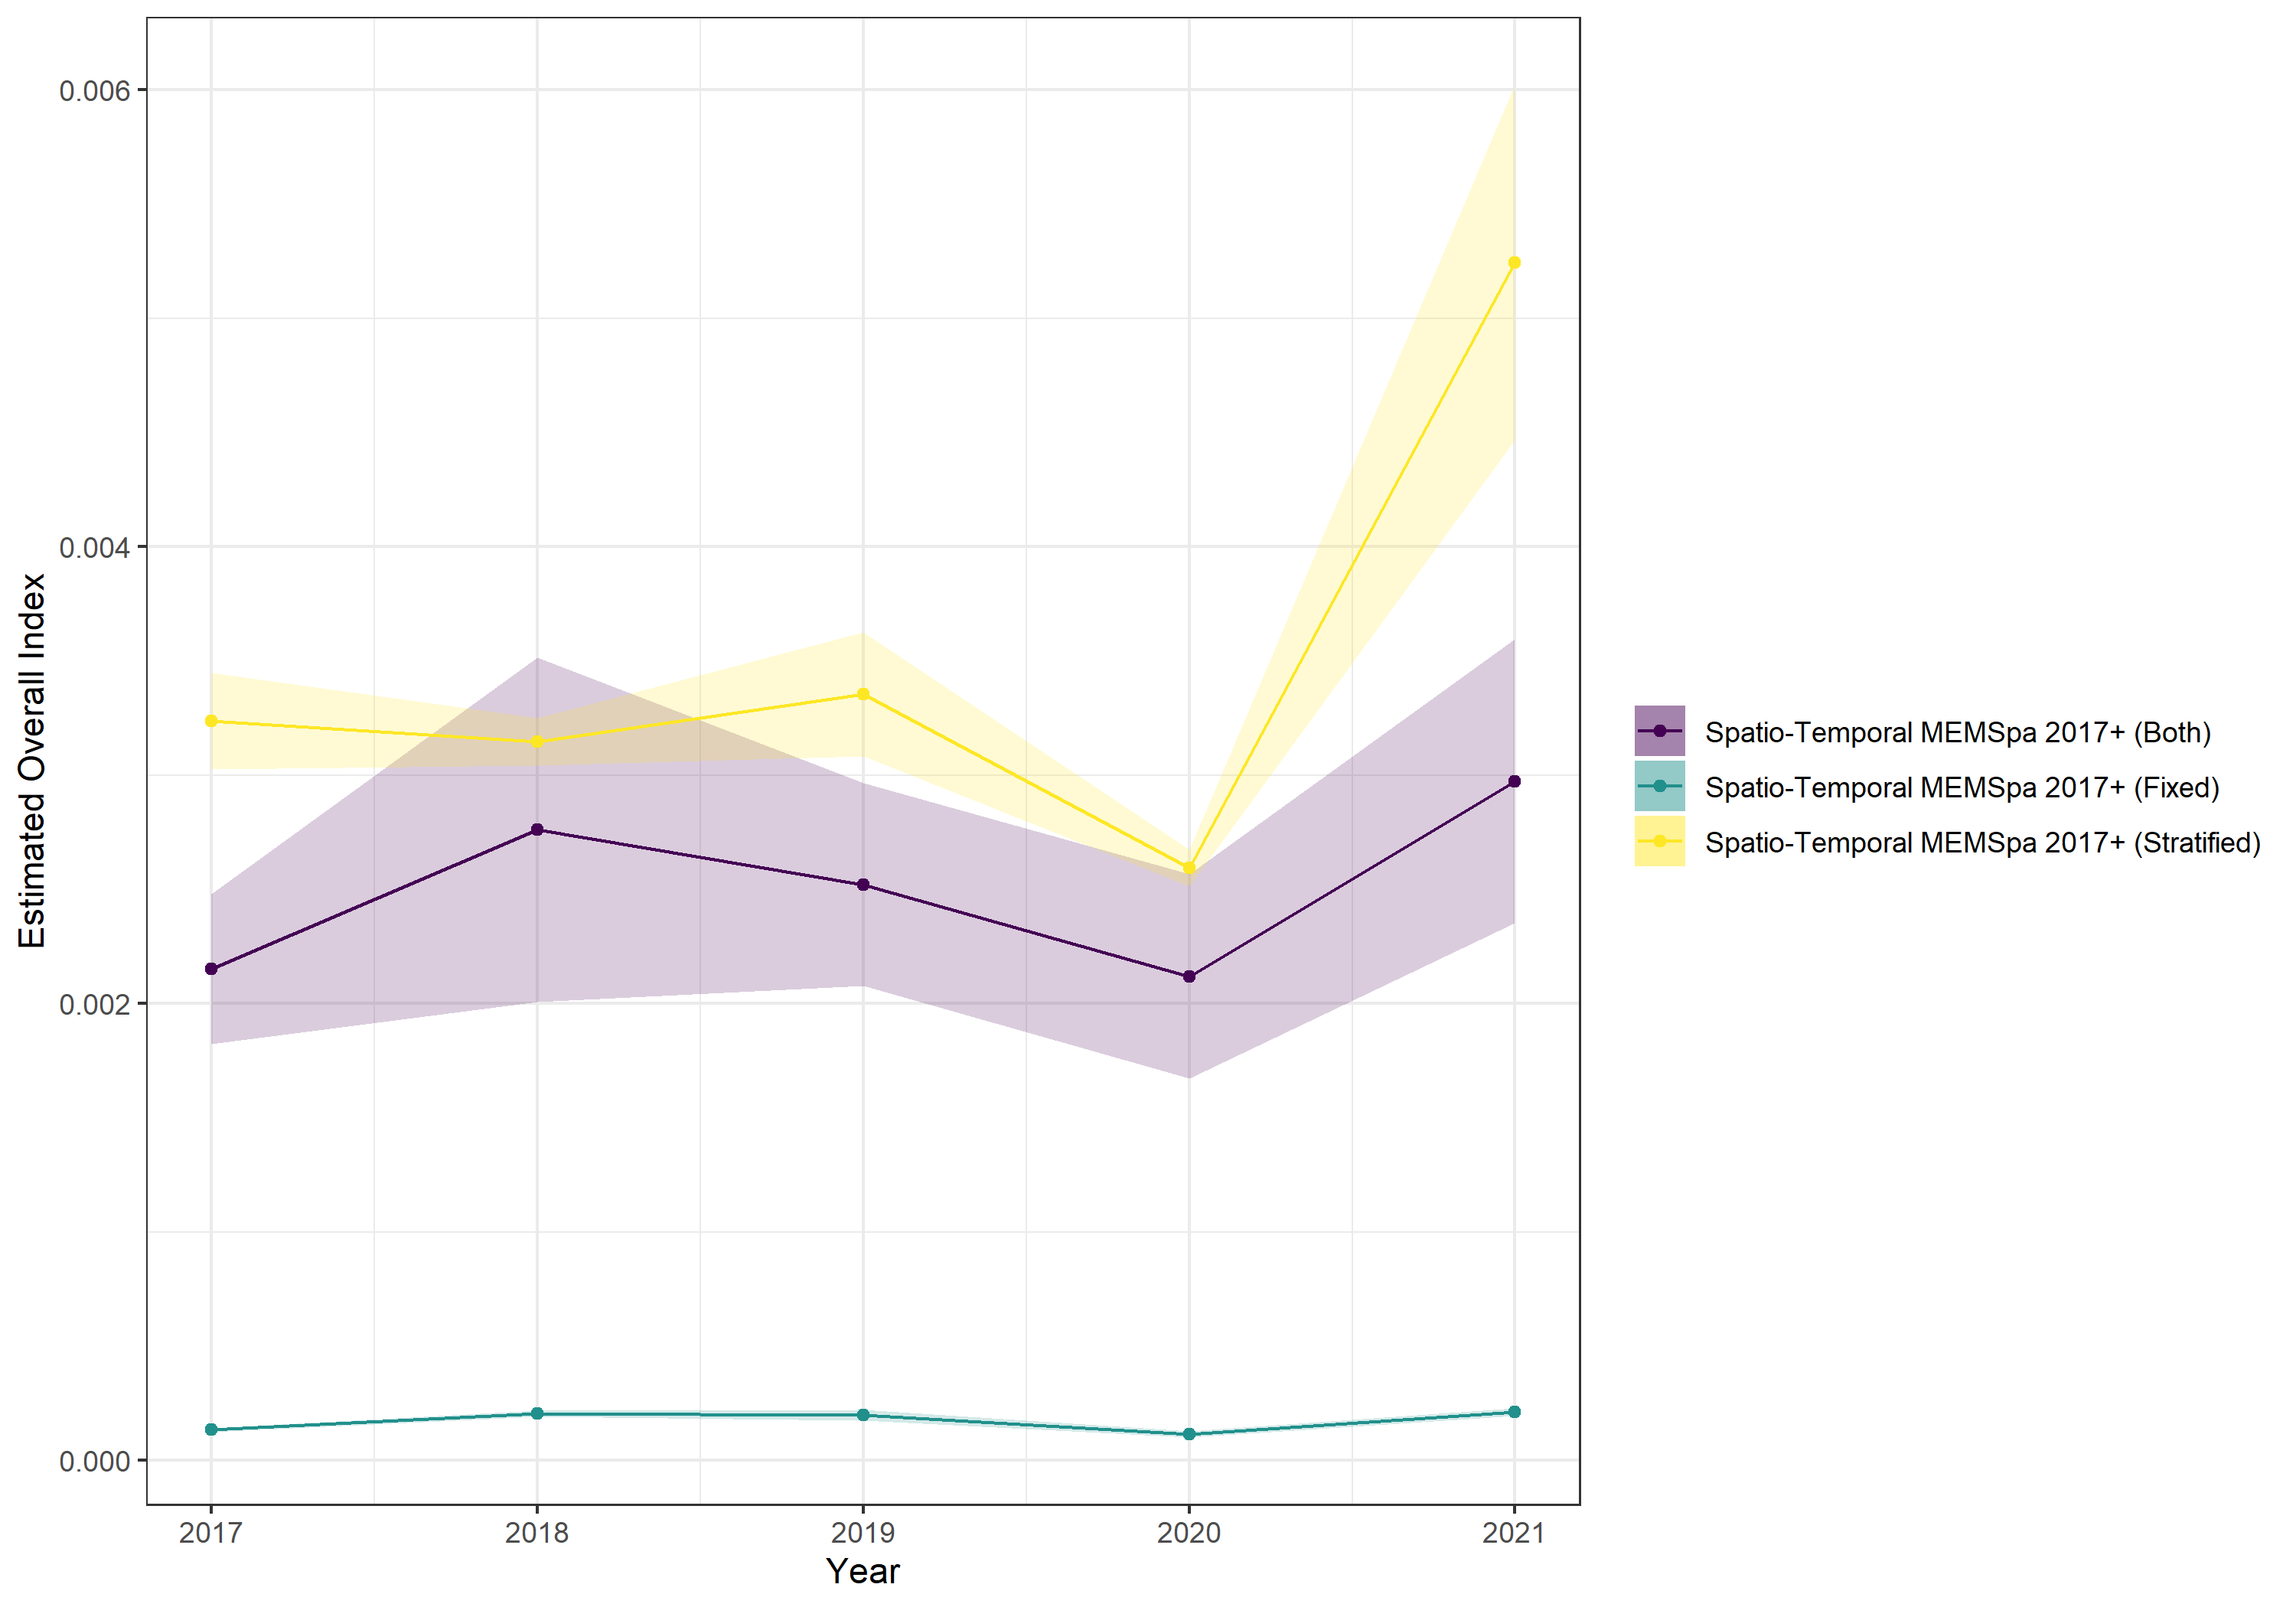
\includegraphics[width=0.75\linewidth]{comp_all_ldant_2017_walk}}{Figure \ref{fig:non-t-indices}} 

}

\caption{Estimated overall index for non-target species using data from the fixed stations and stratified survey design both together and separately between 2000 and 2021 and 2017 and 2021. The uncertainty around the model fits represent +/- 1 standard error.}\label{fig:non-t-indices}
\end{figure}
Looking at the outcomes spatially for the fit with both datasets, the locations of halibut high catch rates appear to generally focus around the Scotian Shelf in the western part of the modelled area, with some spikes around the Laurentian Channel in the middle and a few isolated spikes on the eastern edge of the modelled area (Figure~\ref{fig:target-spat}). For non-target catch rates, the highest spikes are consistently located on the western edge of the area towards the Gulf of Maine and the Bay of Fundy, with other less common spikes located east of the Laurentian Channel. The spatial outcomes from the fit with just the fixed stations has similar patterns (figures in Appendix 2).
\begin{figure}[htb]

{\centering \pdftooltip{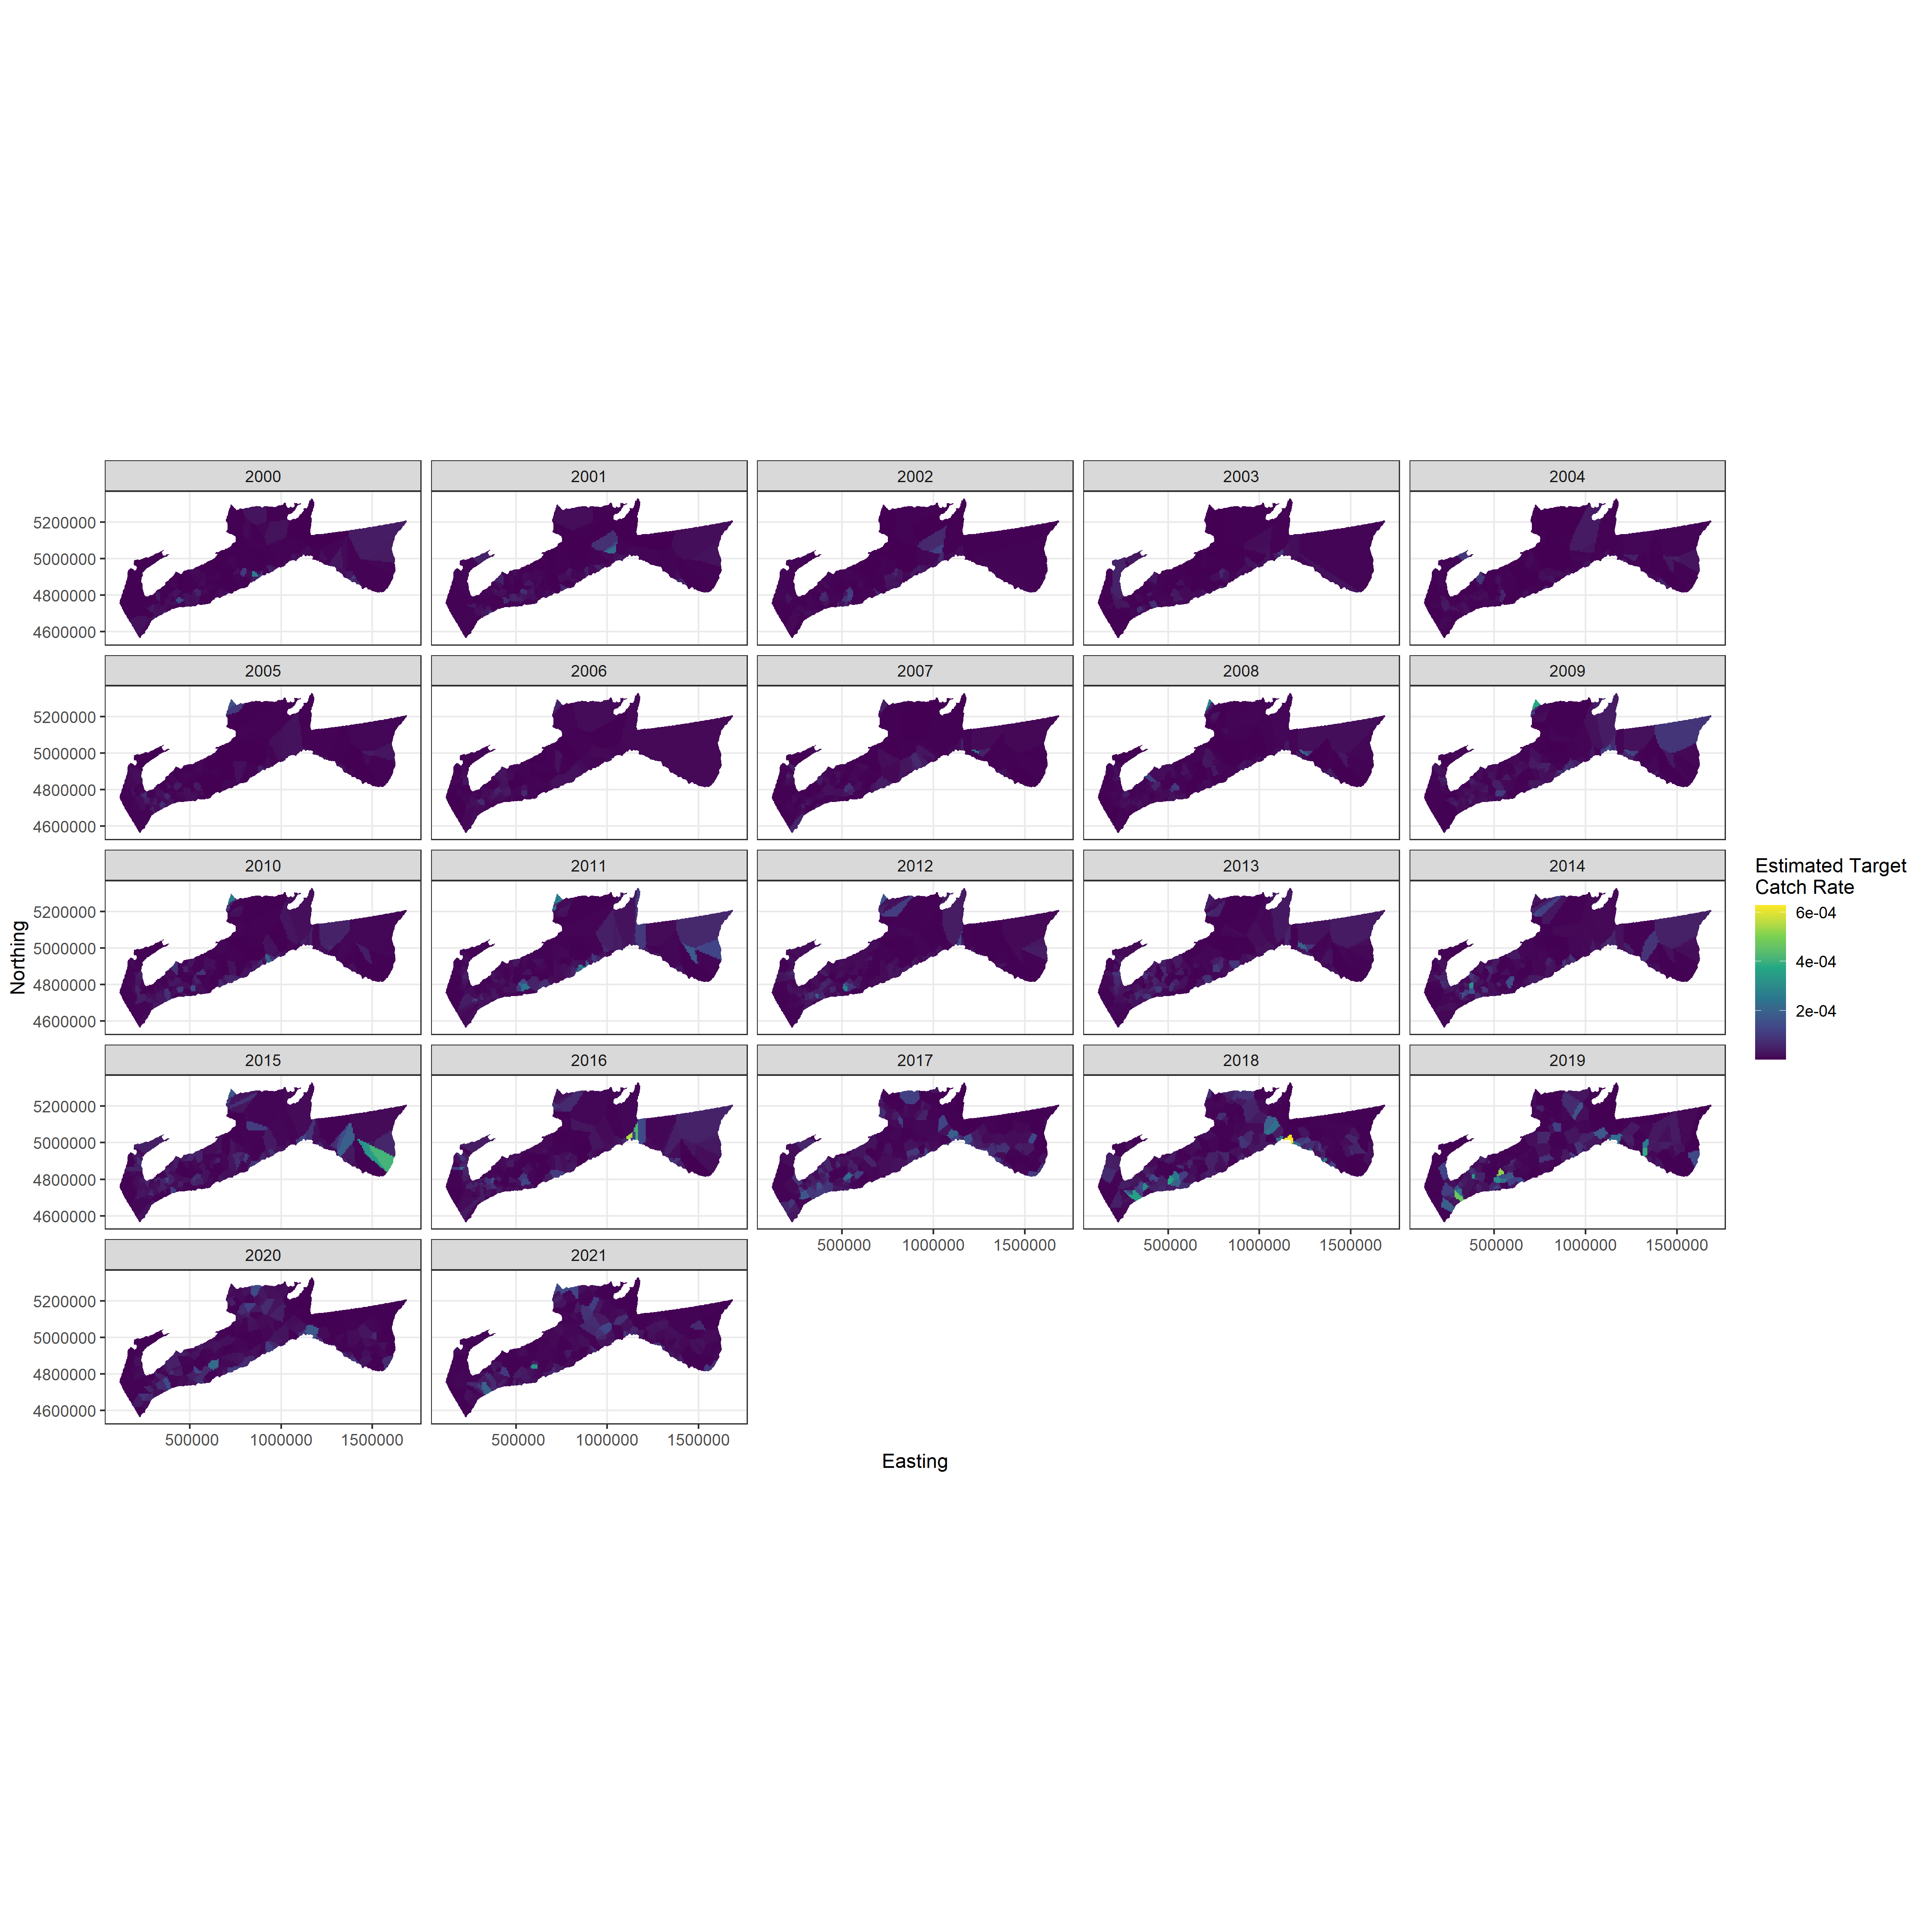
\includegraphics[width=1\linewidth]{all_ldat_both_data}}{Figure \ref{fig:target-spat}} 

}

\caption{Station-specific estimated target species catch rates obtained using data from both the fixed stations and stratified survey design.}\label{fig:target-spat}
\end{figure}
\begin{figure}[htb]

{\centering \pdftooltip{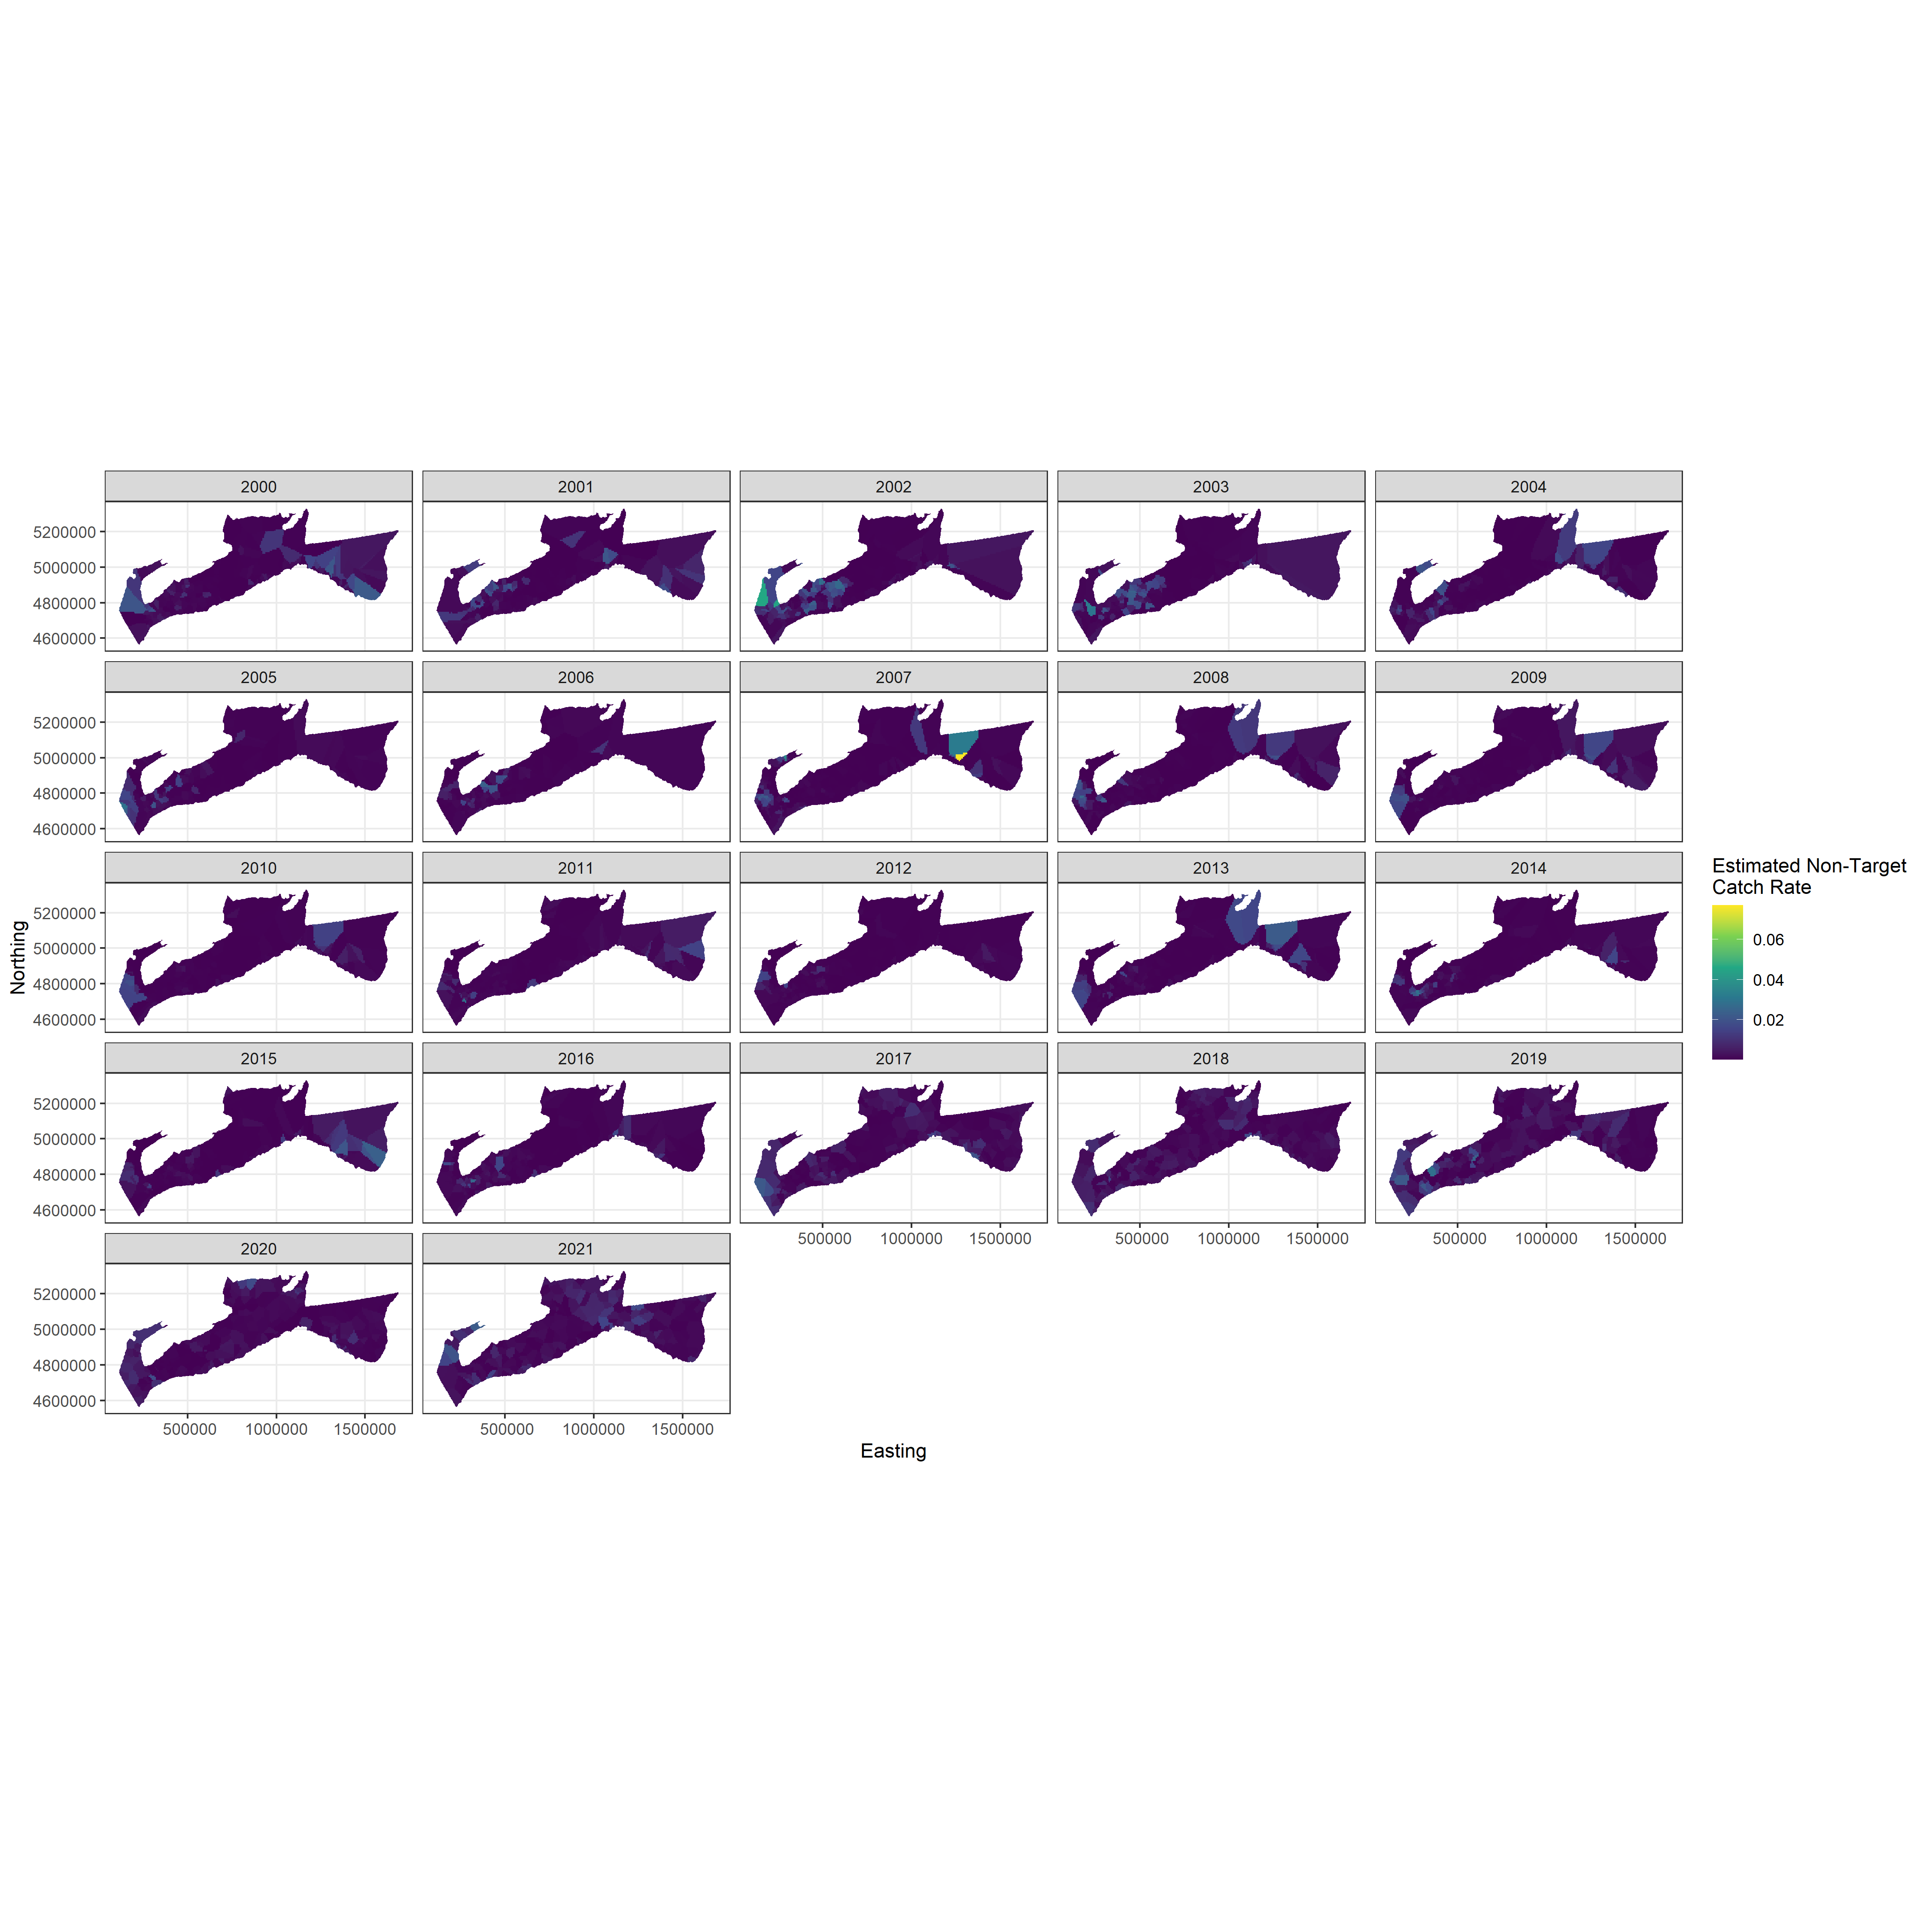
\includegraphics[width=1\linewidth]{all_ldant_both_data}}{Figure \ref{fig:non-target-spat}} 

}

\caption{Station-specific estimated non-target species catch rates obtained using data from both the fixed stations and stratified survey design.}\label{fig:non-target-spat}
\end{figure}
\hypertarget{persistence}{%
\subsection{Persistence}\label{persistence}}

The persistence index of the spatial pattern for target species (halibut) indicate that the fixed stations are extremely likely (\textgreater98\%, see table in Li et al. (\protect\hyperlink{ref-Li2015}{2015})) to capture the changes over time of this population abundance as the index is extremely low for all combination of years. However, the persistence of non-target species exhibits a different pattern (Figure~\ref{fig:persist}) wherein there appears to be a spatial shift in their distribution between early in the time series (mid-2000s) and the peak halibut abundance late in the time series (2017 to 2020). This would represent a high chance that the fixed stations would miss changes in their distribution which, due to the nature of the multinomial model, would impact the estimation of target catch rates. Figure~\ref{fig:rand-int} shows some evidence of this happening in that the expected catch rate for non-target species increases in the late 2010s when the stratified data is included, but not when only the fixed stations are analyzed.
\begin{figure}[htb]

{\centering \pdftooltip{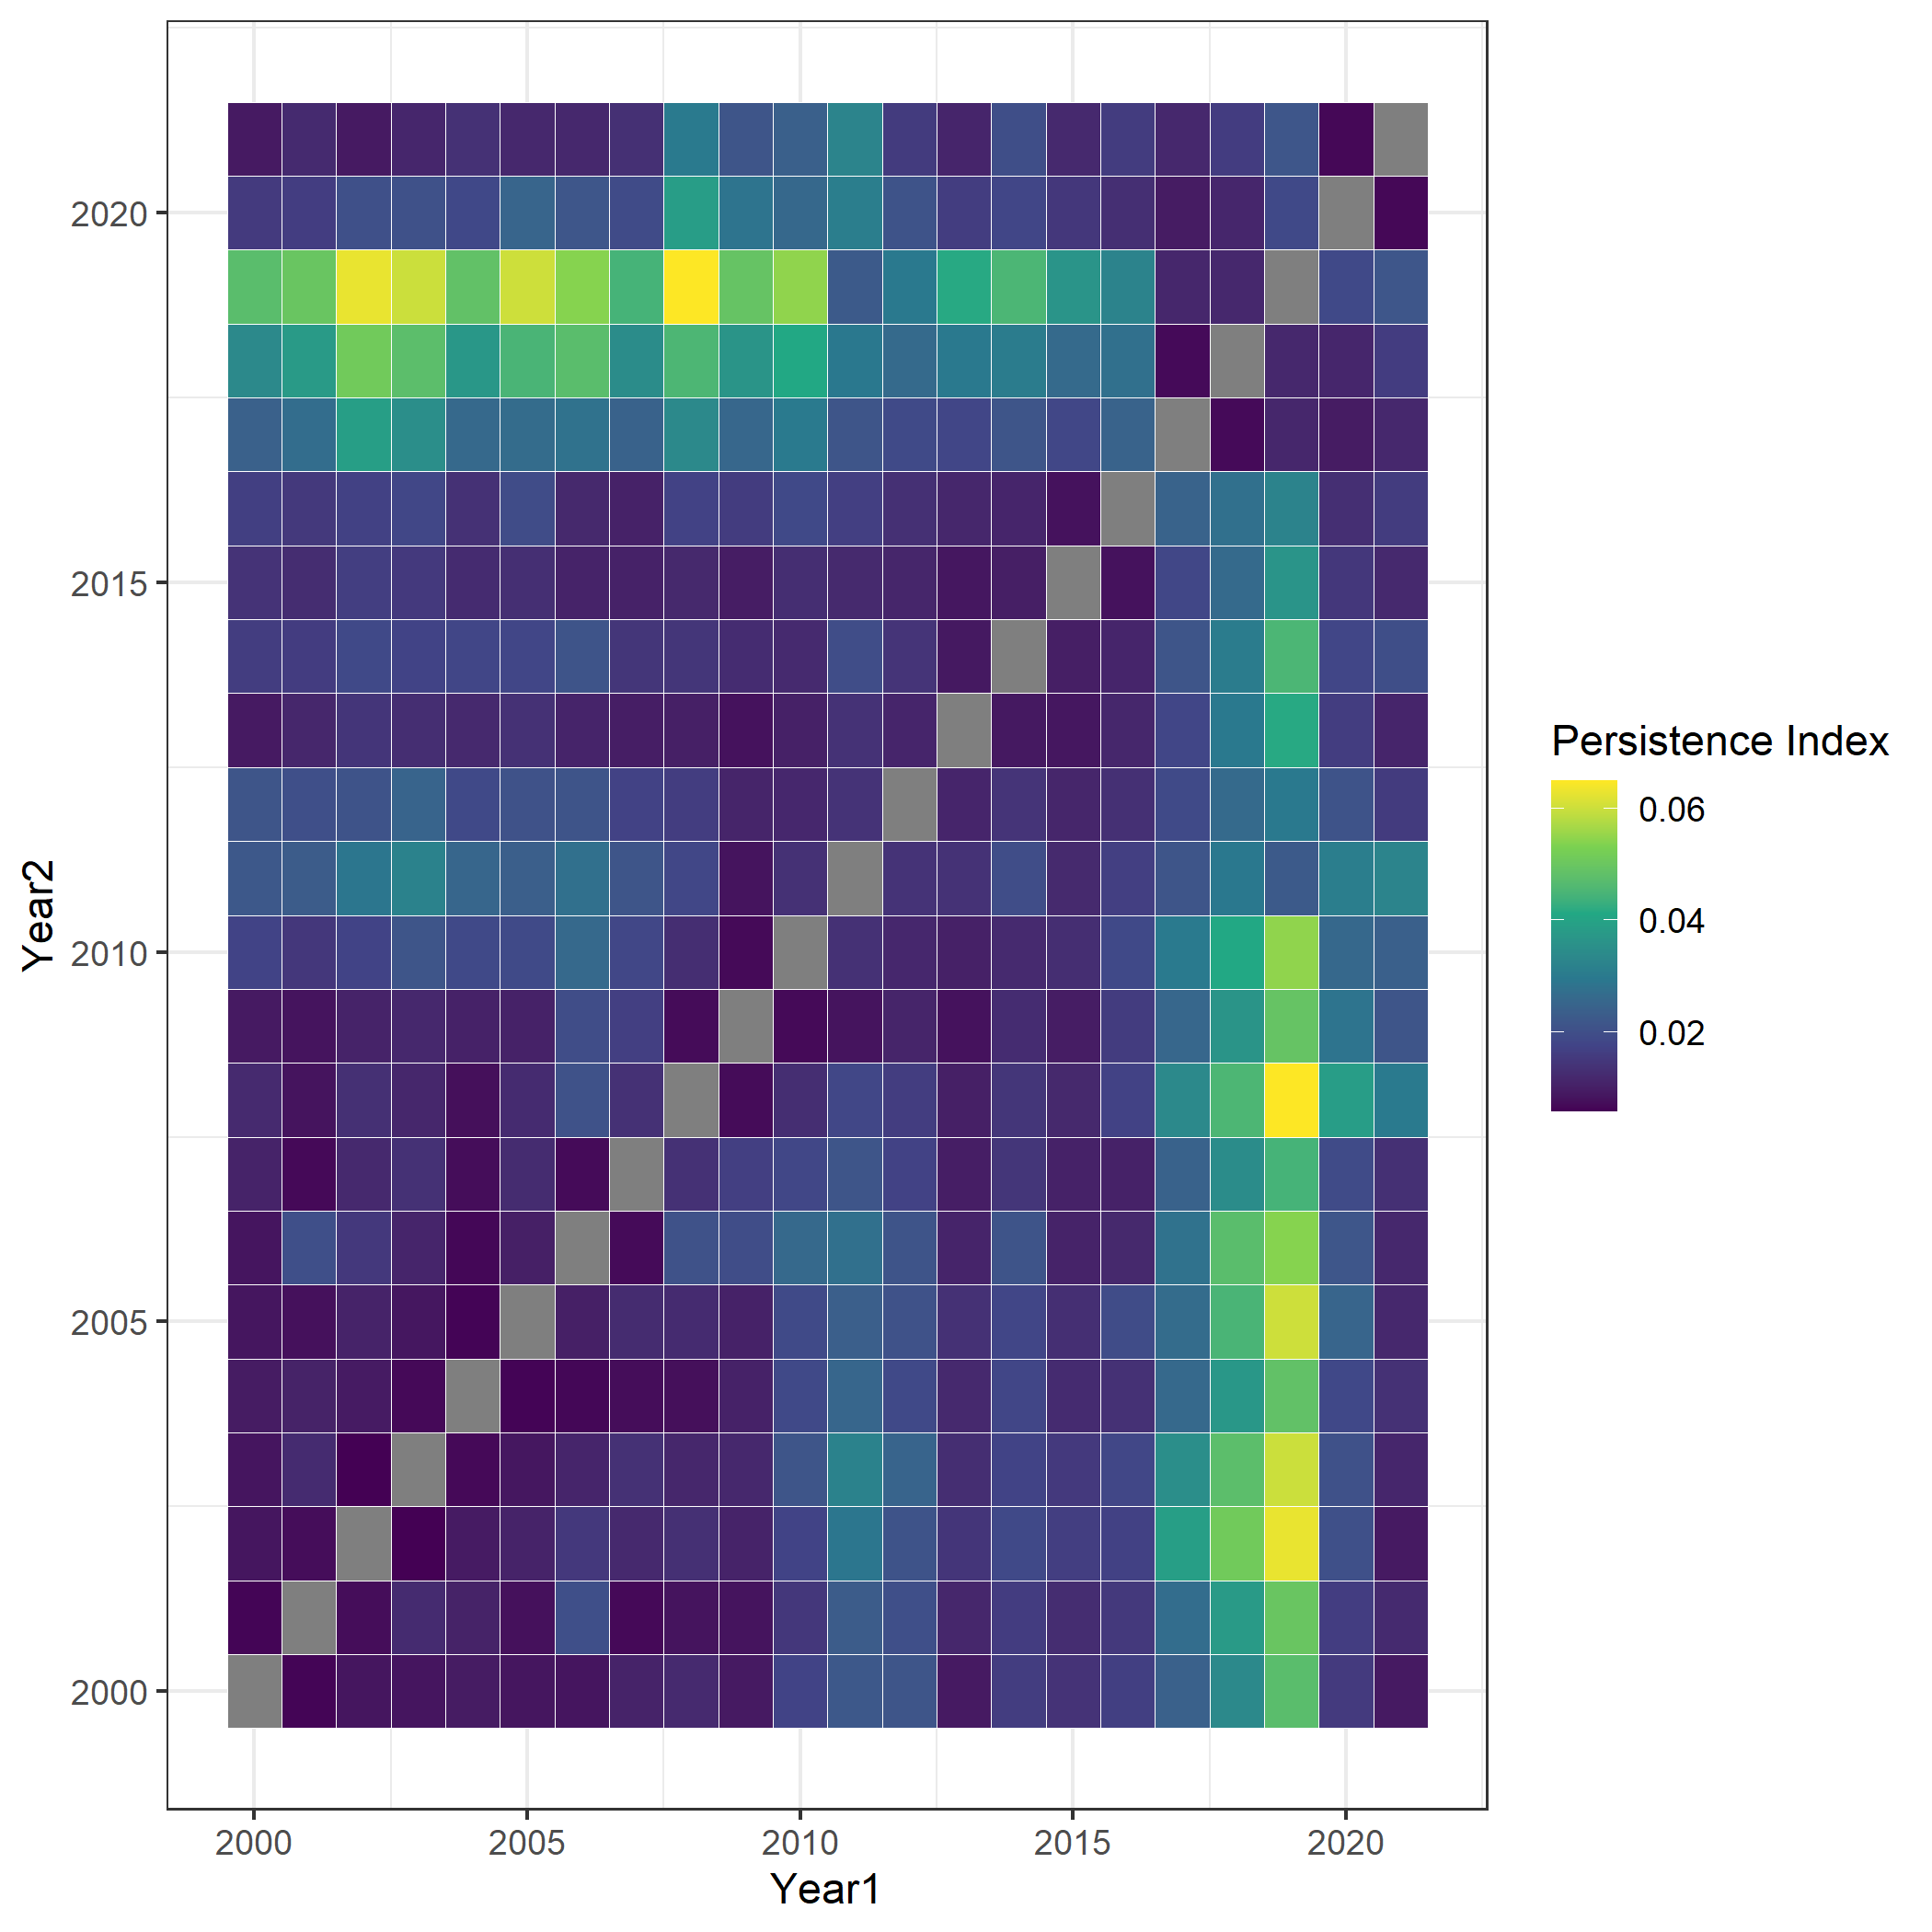
\includegraphics[width=0.6\linewidth]{persist_raster_plot_walk}}{Figure \ref{fig:persist}} \pdftooltip{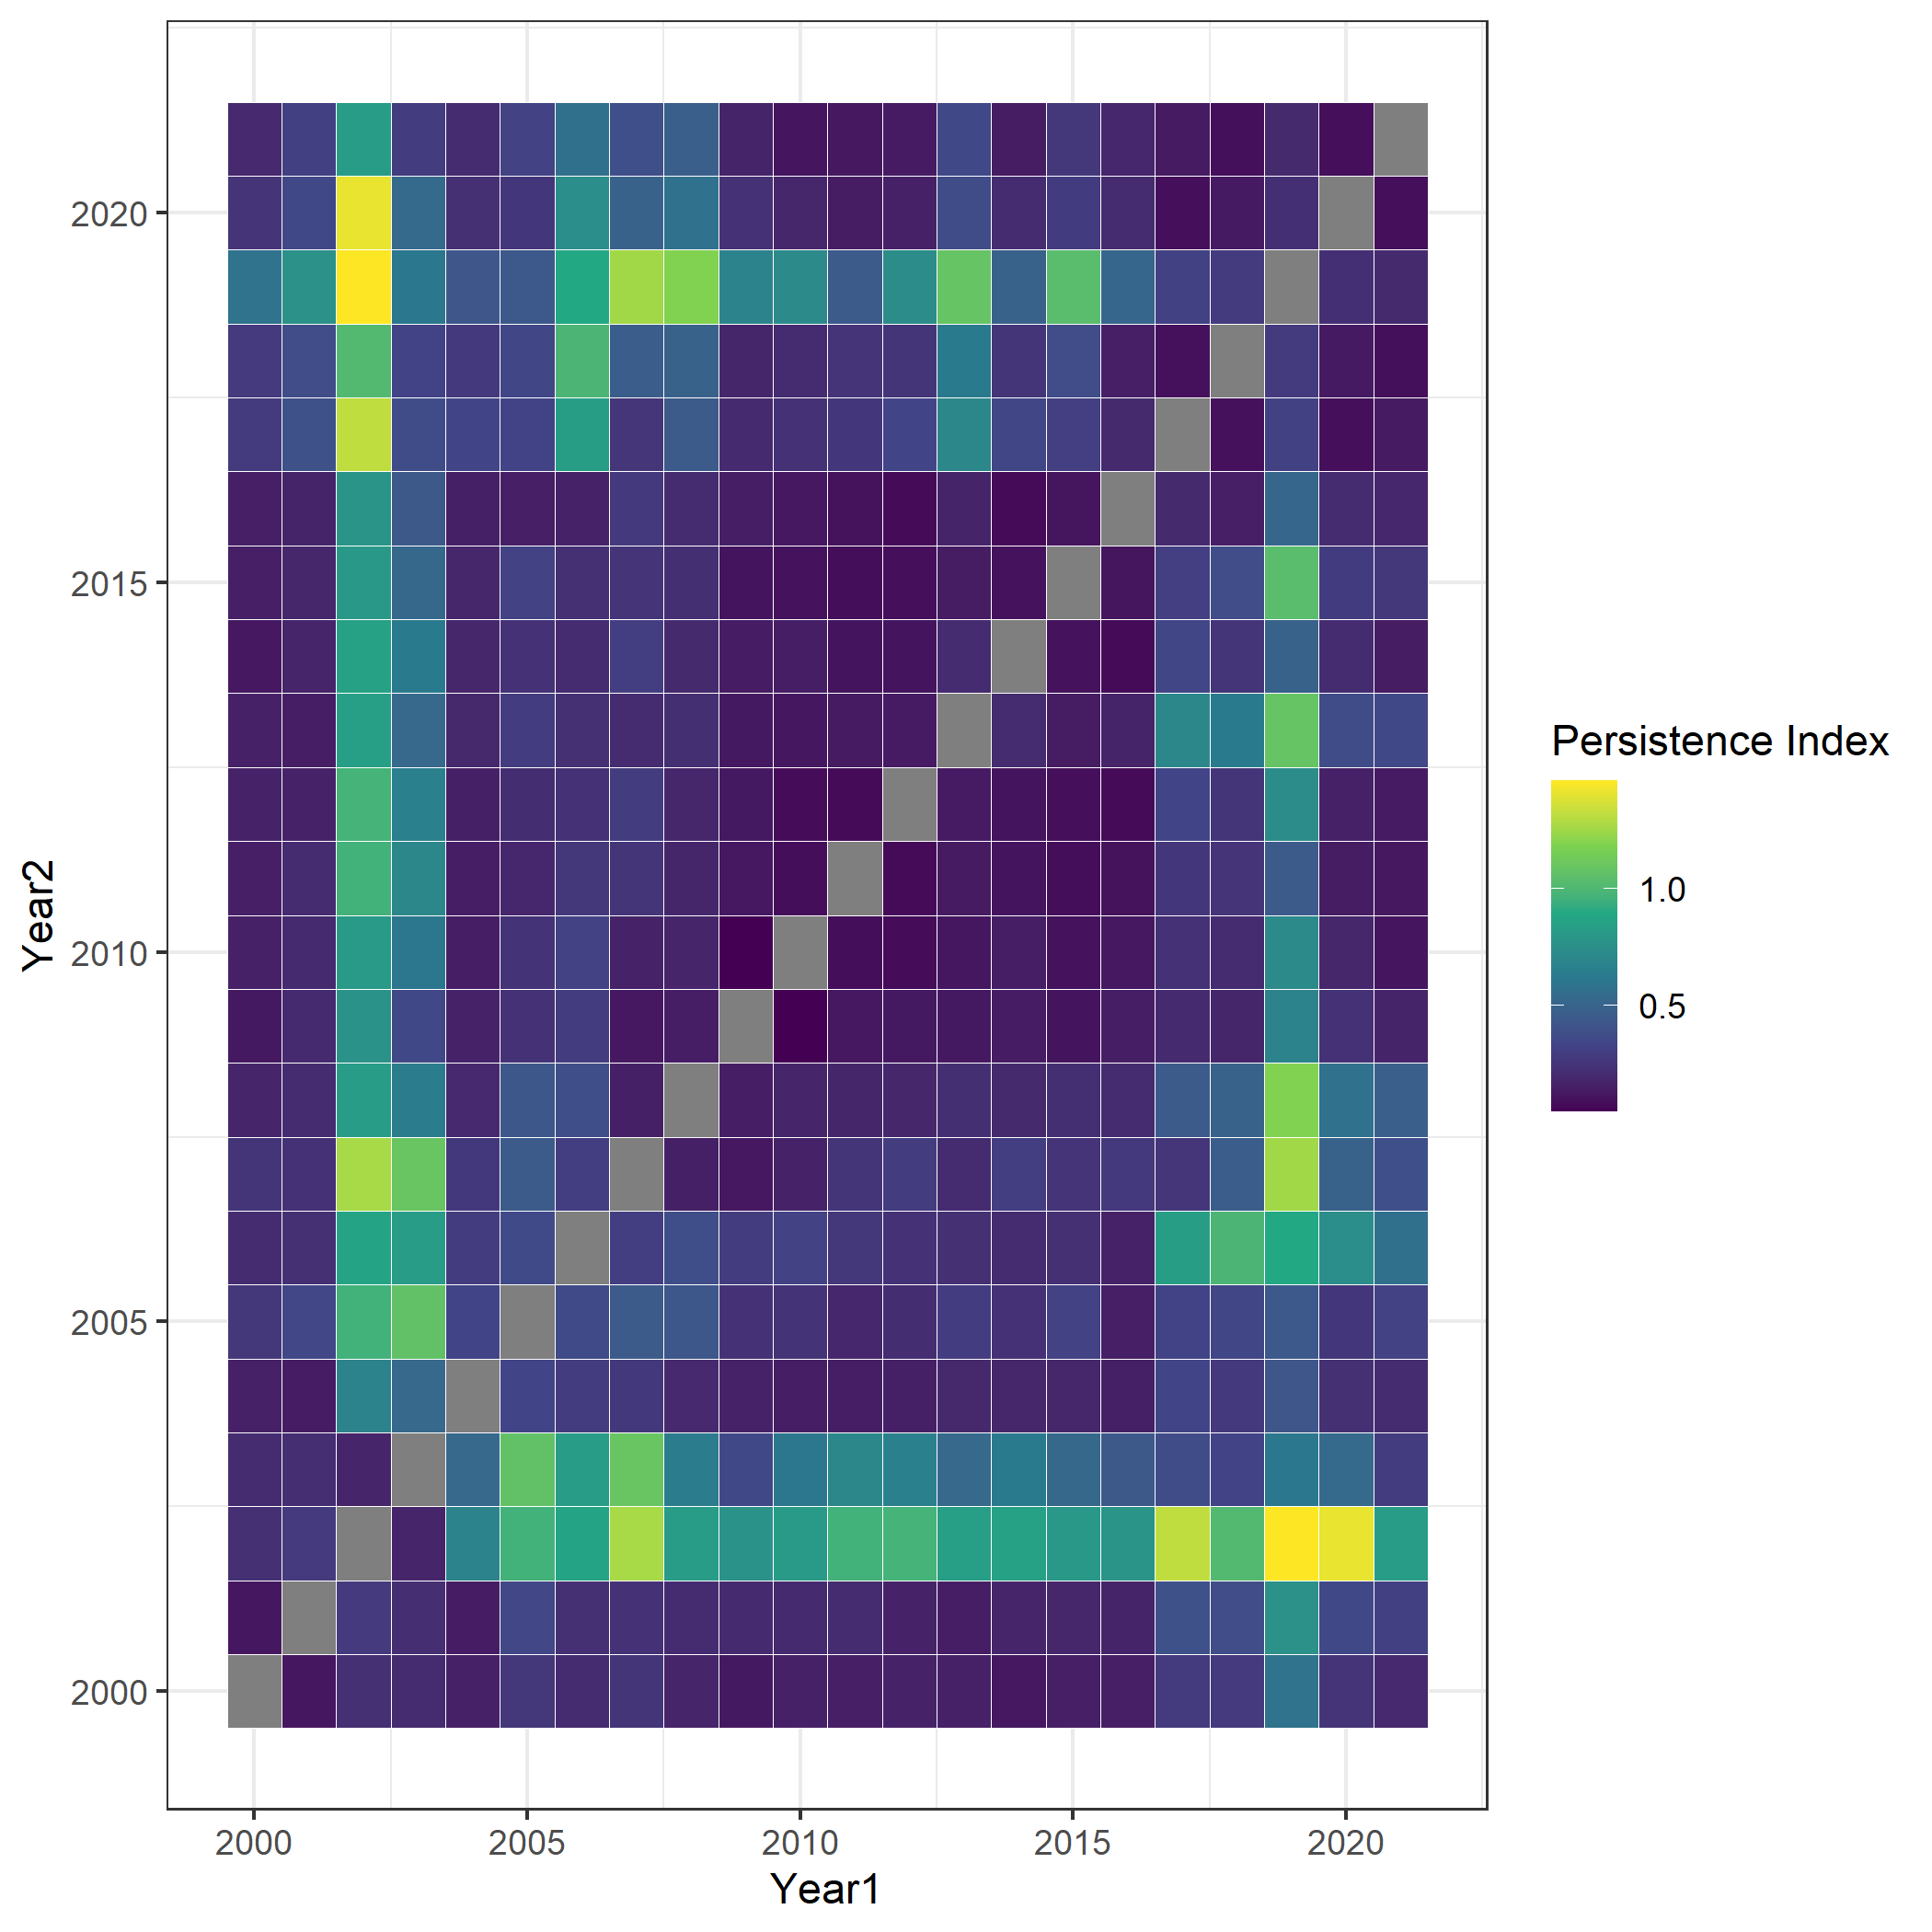
\includegraphics[width=0.6\linewidth]{persist_nt_raster_plot_walk}}{Figure \ref{fig:persist}} 

}

\caption{Persistence index between years for target species (top panel) and non-target species (bottom panel) catch rates.}\label{fig:persist}
\end{figure}
\hypertarget{discussion}{%
\section{Discussion}\label{discussion}}

This novel spatio-temporal MEM is able to successfully capture the changes of the halibut distribution and abundance over time and space for all available data with the exception of the first two years, including two different types of survey designs. It is the only model examined within that is able to include all this information in a unified framework while extracting the maximum amount of information from the available data as possible. Furthermore, since this model is able to output both station-specific estimated catch rate and an overall estimated catch rate for the entire region, it both increases the amount of information available to manage this fishery while being directly comparable to current methods utilized to obtain an index of abundance.

The current stock assessment model requires the indices of abundance to be biomass instead of numbers of fish caught or catch rates (DFO \protect\hyperlink{ref-DFO2021}{2021}), meaning that the estimated catch rates from this model cannot be directly utilized by this model. As the dataset contain average fish weight by tow, it is a potential transformation away from having catch rates in biomass per hook per minute instead of in number of fish, which are then much more applicable and can still retain and propagate uncertainties forward through the delta method (Bickel and Doksum \protect\hyperlink{ref-Bickel2015}{2015}). \textbf{However, more work is necessary to be able to obtain the biomass output as stations that did not catch any halibut will still have an expected catch rate (albeit extremely low), but no fish weight associated with it, meaning that thought has to be put into how one would transform these low catch rates into biomass.}

Similarly to previous versions of the MEM, our spatio-temporal MEM and our analysis of its performance on the Atlantic halibut fishery emphasizes the importance of accounting for the abundance of non-target species for a multivariate approach. The inability to estimate the probability of non-target escapes without hook condition information, illustrated very well in the fits that do not include the stratified dataset, demonstrates this impact very well. This underlines the importance of having a reliable estimate of the abundance of these non-target species. The modelling output themselves show that overestimating the abundance of these non-target species will likely result in an underestimation of the halibut population abundance, underestimating their abundance would likely result in the opposite, and completely ignoring them is likely to result in unpredictable and variable biases.

A key outcome from this analysis is that there is evidence that, while the fixed stations were likely appropriate to capture the large changes of halibut abundance, they are likely not capturing changes in distribution and abundance of non-target species which will subsequently impact the estimation of halibut abundance. As the longline gear catches a great number of other species (e.g., cod, dogfish, etc.), it is not too surprising that their overall joint spatial distribution would shift which, as we have shown, would then have an impact on the halibut catch rates. The timing of the implementation of the stratified random sampling design (2017) therefore appears to be fortunate, as those are the years where the fixed stations seem to be missing the shift in abundance of non-target species. This new design does capture these changes, allowing the model to therefore get a more accurate estimate of the underlying halibut abundance. Furthermore, the estimates from the stratified random design will only get more accurate and precise as years are added into the time series.

While it was developed for this specific longline survey, this model could easily be applied to any longline fisheries or other passive sampling gear that would be impacted by hook or bait competition and promises to improve indices of abundance used for stock assessment models. Depending on the fishery, it could be of great value to further modify the multinomial equation used by our approach to expand on the non-target species to include multiple specific species. More specifically, if there are a finite amount of other species being caught aside from the target, it would likely lead to improvements in estimated catch rates for the target species.

\begin{appendices}
\counterwithin{figure}{section}
\counterwithin{table}{section}
\counterwithin{equation}{section}

\clearpage

\section{}
\label{app:first-appendix}

\flushright{2 September 2021}

\centering

\textbf{Terms of Reference (TOR)} \flushleft

Statistical innovations for obtaining and validating Atlantic halibut longline survey indices of exploitable biomass through implementation of a multinomial, hook occupancy model.

\textbf{Estimated Value}

The total value of any contract(s) emanating from this TOR is \$10000 (4 months).

\textbf{Objectives of the Requirement}

To extend the proposed spatial modeling to include the fix station and explore spatial temporal model to provide an index over time from the beginning of the survey until current time.

\textbf{Background, Assumptions and Specific Scope of the Requirement}

Together, the Atlantic Halibut Council and the Department of Fisheries and Oceans Canada (DFO) have used an annual longline survey to monitor Atlantic halibut exploitable biomass since 1988. The survey was originally stratified into areas of Low, Medium and High catch based on data from commercial fishing logs (1995-1997). Stratified estimates were used until the assessment by Trzcinski et al.~(2009) when the stratification system was no longer utilized (although the strata were still part of the survey design). Starting in 2009, a standardized catch rate calculated from a negative binomial (NB) generalized linear model (GLM) replaced the stratified estimate of mean weight per standard longline set (den Heyer et. al., 2013).

The simple stratified mean adjusted catch rate and the NB GLM both assume that halibut are the only species being caught by the longline hooks with no accounting for other species competing for hooks. In addition, these methods implicitly assume that all hooks that do not have halibut would still have been able to catch halibut had there been more of these fish in the area. However, some number of hooks will be occupied by species other than halibut and other hooks will be empty with bait still attached or missing. Smith (2016) recently recommended replacing the NB GLM with a multinomial model that accounted for both the number of halibut caught, and the number of hooks occupied by other species or missing bait.

The Atlantic halibut longline survey was designed to provide an annual index of abundance (numbers or weights) to monitor the status of the stock for management purposes. Based on the work has been done by now, it is useful to extend that spatial modeling to include the fix station as well, also explore spatial temporal model to provide an index over time from the beginning of the survey until current time. In other words, we will have one index to include in our assessment model for the longline survey data both from fixed station and stratified random.

\textbf{Tasks, Activities and Deliverables}

The deliverables for the project will be to:
\begin{enumerate}
\def\labelenumi{\arabic{enumi})}
\item
  Develop spatiotemporal multinomial model for stratified random station survey 2017-2020
\item
  Develop spatiotemporal multinomial model for the fixed station survey data 1998-2020 (app 230 station 1998-2016 and 100 stations 2017-2020)
\item
  Develop a spatiotemporal model that simultaneously analyzes the data from the four years, 2017-2020, for which there are both fixed and stratified random station data.
\item
  Develop a spatiotemporal model for the entire time series, 1998-2020, of fixed station and random survey data
\item
  A technical report.
\end{enumerate}
\textbf{Expected Start and Completion Dates}

All work will be completed between September 2021 and January 2022. The weekly number of hours worked will vary over that timeframe, as agreed upon between DFO and Dalhousie University (Dr.~Joanna Mills Flemming).

\textbf{Contingencies}

If the tasks/deliverables are in jeopardy due to unforeseen circumstances such as student leaving the project or because of other complications or poor work quality, the Scientific Authorities will proceed with the project goals through contracts to other students and/or conduct the analyses themselves.

\textbf{Reporting Requirements}
\begin{enumerate}
\def\labelenumi{\arabic{enumi}.}
\item
  Basic updates from the student on how work is progressing are required weekly by email or phone with the Scientific Authorities.
\item
  At the end of work, a detailed report, relating the progress of the project with respect to the identified deliverables, will be provided to the Project Authorities. This report must be sufficiently detailed that the Project Authorities are able to evaluate whether the progress of the project is sufficient that contingency plans, as outlined above, do not need to be implemented.
\end{enumerate}
\textbf{Change Management Procedures}

Changes to the scope of the project will be made through agreement by all parties and documented through email correspondence.

\textbf{Other Terms and Conditions}

Authorities

Scientific Authorities

Dr.~Joanna Mills Flemming and Dr.~Bruce Smith

Department of Mathematics and Statistics \textbar{} Dalhousie University

902-494-2572 PO Box 15000 \textbar{} Halifax NS B3H 4R2 Canada

Contracting Authority (Dalhousie University)

Miriam Breslow

HR Advisor, Academic Staff Relations

Human Resources \textbar{} Dalhousie University

902-494-2965

Henry Hicks Administration Building, Room 150

PO Box 15000 \textbar{} Halifax, NS B3H 4R2 Canada

Project Authorities (DFO and Atlantic Halibut Council)

Dr.~Lingbo Li and Dr.~Cornelia (Nell) den Heyer

Population Ecology Division, Science Branch,

Fisheries and Oceans Canada,

P.O. Box 1006, Dartmouth, NS B2Y 4A2

\link{mailto:Brendan.Wringe@dfo-mpo.gc.ca}{\nolinkurl{Brendan.Wringe@dfo-mpo.gc.ca}}

Mr.~Bruce Chapman

Atlantic Halibut Council

\link{mailto:bchapman@sympatico.ca}{\nolinkurl{bchapman@sympatico.ca}}

\textbf{DFO and Atlantic Halibut Council Obligations}

DFO and the Atlantic Halibut Council will provide all relevant fisheries and biological data and access to staff members or fishers who will be available for advice on, and participate in, the proposed activities. DFO will provide training in the data and current modelling procedures as background to the work.

\textbf{Location of Work}

Work will be conducted at Dalhousie University or with the other parties as expertise or third-party funding sources requires.

\textbf{Remuneration}

Invoicing will be monthly; an initial invoice in September 2021 and a final invoice in January 2022.

\textbf{References}

Armsworthy, S, Wilson, S, Mohn, R. 2006. Atlantic halibut on the Scotian Shelf and Southern Grand Banks (NAFO Division 3NOPs4VWX5Zc) -- Industry/DFO longline survey results to 2005. DFO Can. Sci. Advis. Sec. Res. Doc. 2006/065. ii +31p.

den Heyer, C, Schwarz, C, and Trzcinski, M. 2013. Fishing and natural mortality rates of Atlantic halibut estimated from multiyear tagging and life history. Trans. Am. Fish. Soc. 143(3): 690-702.

Etienne, M, Obradovich, S, Yamanaka, K, and McAllister, M. 2013. Extracting abundance indices from longline surveys: a method to account for hook competition and unbaited hooks. arXiv 1005.0892v3:1-35.

Smith, S. 2016. Review of the Atlantic halibut longline survey index of exploitable biomass. Canadian Technical Report of Fisheries and Aquatic Sciences 3180.

Thorson, J, Ianelli, J, Munch, S, Ono, K, Spencer, P. 2015b. Spatial delay-difference models for estimating spatiotemporal variation in juvenile production and production abundance. Can. J. Fish. Aquat. Sci. 72 (12), 1897-1915. doi: 10.1139/cjfas-2014-0543.

Thorson, J, Skaug, H, Kristensen, K, Shelton, A, Ward, E, Harms, J, Benante, J. 2015a. The importance of spatial models for estimating the strength of density dependence. Ecology 96 (5), 1202--1212. doi: 10.1890/14-0739.1.sm

Thorson, J, Shelton, A, Ward, E., Skaug, H. 2015c. Geostatistical delta-generalized linear mixed models improve precision for estimated abundance indices for West Coast groundfishes. ICES J. Mar.~Sci. 72, 1-11. doi: 10.1093/icesjms/fst176.

Trzcinski, M, Armsworthy, S, Wilson, S, Mohn, R, Fowler, M and Campana, S. 2009. Atlantic halibut on the Scotian Shelf and Southern Grand Banks (NAFO Division 3NOPs4VWX5Zc) -- Industry/DFO longline survey and tagging results to 2008. DFO Canadian Scientific Advisory Sec. Res. Doc. 2009/026. vi +43p

\clearpage

\section{}
\label{app:second-appendix}
\begin{figure}[htb]

{\centering \pdftooltip{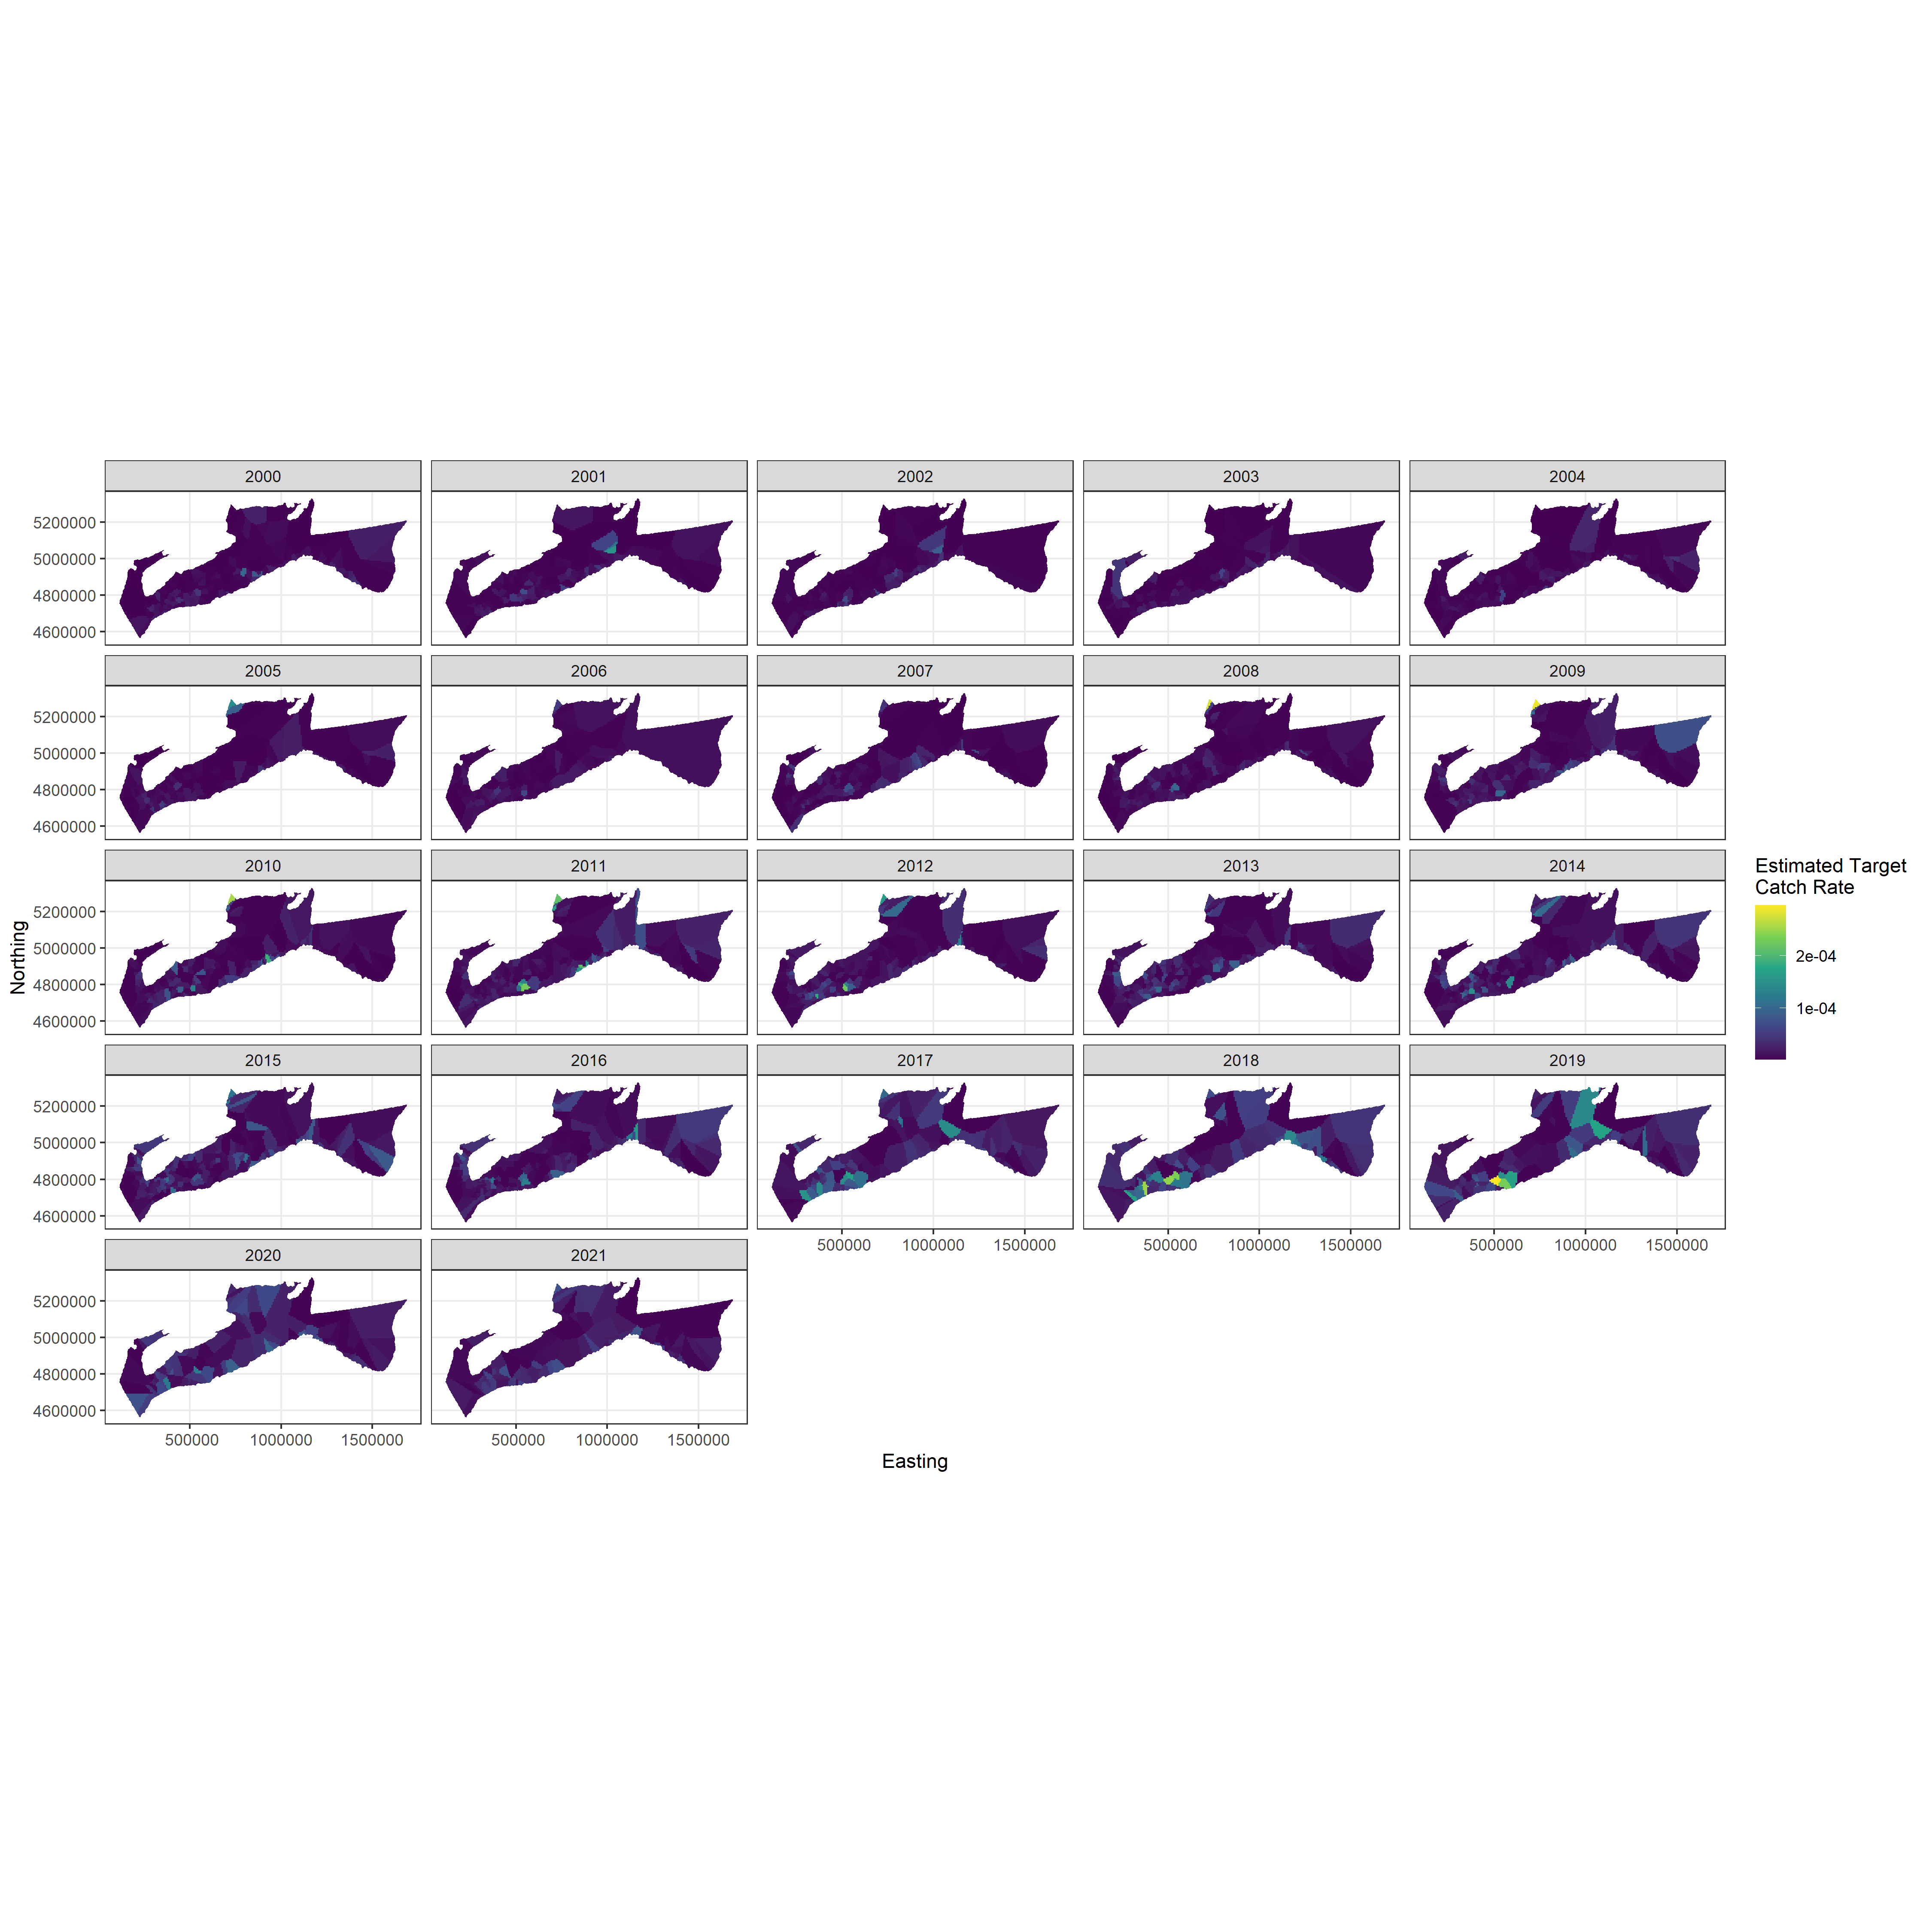
\includegraphics[width=1\linewidth]{1phi_no_cons_mean_all_ldat}}{Figure \ref{fig:target-spat-fixed}} 

}

\caption{Station-specific estimated target species catch rates obtained using data from only the fixed stations.}\label{fig:target-spat-fixed}
\end{figure}
\begin{figure}[htb]

{\centering \pdftooltip{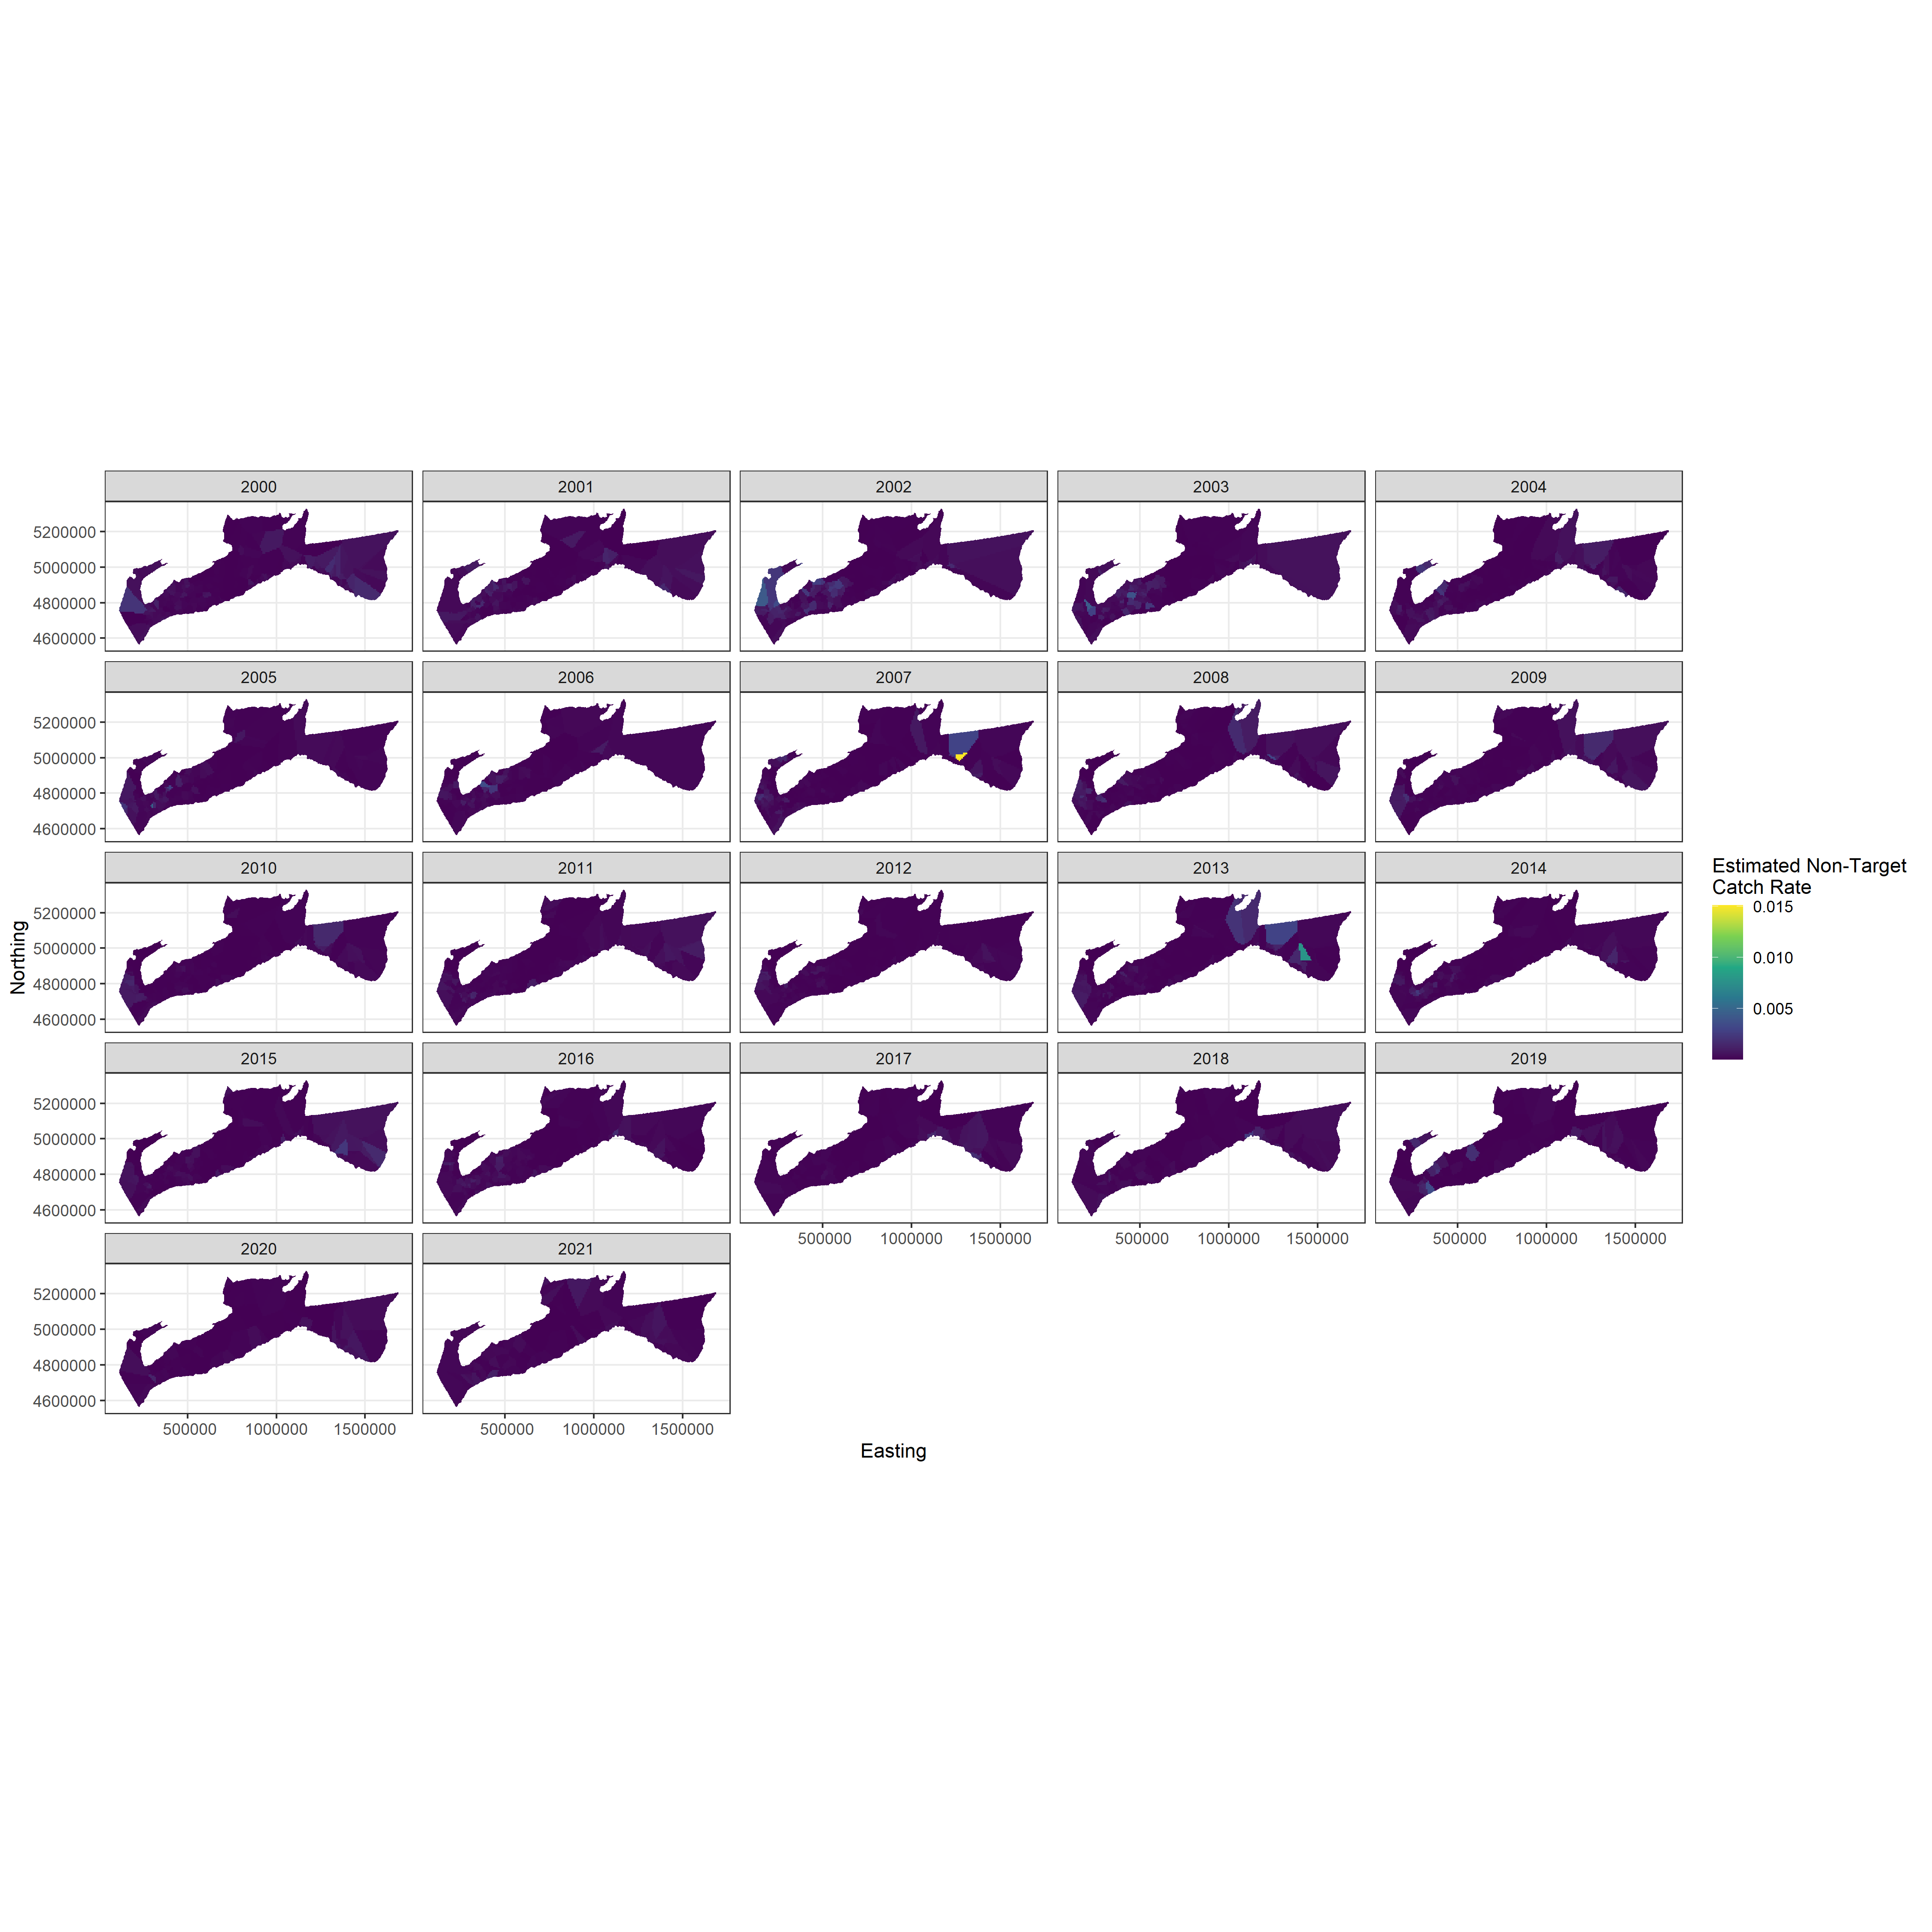
\includegraphics[width=1\linewidth]{1phi_no_cons_mean_all_ldant}}{Figure \ref{fig:non-target-spat-fixed}} 

}

\caption{Station-specific estimated non-target species catch rates obtained using data from only the fixed stations.}\label{fig:non-target-spat-fixed}
\end{figure}
\end{appendices}

\clearpage

\hypertarget{references}{%
\section{References}\label{references}}

\noindent \vspace{-2em} \setlength{\parindent}{-0.2in} \setlength{\leftskip}{0.2in} \setlength{\parskip}{8pt}

\hypertarget{refs}{}
\leavevmode\hypertarget{ref-Akaike1974}{}%
Akaike, H. 1974. A new look at the statistical model identification. IEEE Trans. Automat. Contr. 19(6): 716--723.

\leavevmode\hypertarget{ref-Bickel2015}{}%
Bickel, P.J., and Doksum, K.A. 2015. Mathematical Statistics: Basic Ideas and Selected Topics, Volumes I. Chapman; Hall/CRC Press.

\leavevmode\hypertarget{ref-Cox2018}{}%
Cox, S., Benson, A., and Doherty, B. 2018. Re-design of the Joint Industry-DFO Atlantic Halibut (Hippoglossus hippoglossus) Survey off the Scotian Shelf and Grand Banks. (DFO Can. Sci. Advis. Sec. Res. Doc. 2018/020.): v + 50 p.

\leavevmode\hypertarget{ref-DenHeyer2015}{}%
den Heyer, C.E., Hubley, B., Themelis, D., Smith, S.C., Wilson, S., and Wilson, G. 2015. Atlantic Halibut on the Scotian Shelf and Southern Grand Banks~: Data Review and Assessment Model Update. Canadian Science Advisory Secretariat Research Document DFO Can. S(2015/051).

\leavevmode\hypertarget{ref-DFO2021}{}%
DFO. 2021. Stock Status Update of Atlantic Halibut (Hippoglossus hippoglossus) on the Scotian Shelf and Southern Grand Banks in NAFO Divisions 3NOPs4VWX5Zc for 2020. Canadian Science Advisory Secretariat (CSAS) (2021/024).

\leavevmode\hypertarget{ref-Doherty2017}{}%
Doherty, B., Cox, S., and Benson, A. 2017. March 2017 Technical Report March 2017 Technical Report. Landmark Fisheries.

\leavevmode\hypertarget{ref-Etienne2013}{}%
Etienne, M.-P., Obradovich, S., Yamanaka, L., and Mcallister, M. 2013. Extracting abundance indices from longline surveys~: method to account for hook competition and unbaited hooks.: 1--35.

\leavevmode\hypertarget{ref-Kai2017}{}%
Kai, M., Thorson, J.T., Piner, K.R., and Maunder, M.N. 2017. Spatiotemporal variation in size-structured populations using fishery data: an application to shortfin mako ( \textless i\textgreater Isurus oxyrinchus\textless/i\textgreater{} ) in the Pacific Ocean. Canadian Journal of Fisheries and Aquatic Sciences 74(11): 1765--1780.

\leavevmode\hypertarget{ref-Kess2021}{}%
Kess, T., Einfeldt, A.L., Wringe, B., Lehnert, S.J., Layton, K.K.S., McBride, M.C., Robert, D., Fisher, J., Le Bris, A., Den Heyer, C., Shackell, N., Ruzzante, D.E., Bentzen, P., and Bradbury, I.R. 2021. A putative structural variant and environmental variation associated with genomic divergence across the Northwest Atlantic in Atlantic Halibut. ICES Journal of Marine Science 78(7): 2371--2384.

\leavevmode\hypertarget{ref-Lee2018}{}%
Lee, L.M., and Rock, J.E. 2018. The forgotten need for spatial persistence in catch data from fixed-station surveys. Fishery Bulletin 116(1): 69--74.

\leavevmode\hypertarget{ref-Li2015}{}%
Li, B., Cao, J., Chang, J.H., Wilson, C., and Chen, Y. 2015. Evaluation of Effectiveness of Fixed-Station Sampling for Monitoring American Lobster Settlement. North American Journal of Fisheries Management 35(5): 942--957.

\leavevmode\hypertarget{ref-Li2022}{}%
Li, L., Hubley, B., Harper, D.L., Wilson, G., and Heyer, C.E. den. 2022. Data review and assessment model update: Assessment of atlantic halibut on the scotian shelf and southern grand banks (nafo divs. 3NOPs4VWX5Zc) data inputs and model. DFO Canadian Science Advisory Secretariat Research Document 2022/nnn: vi + xx p.

\leavevmode\hypertarget{ref-Li2019}{}%
Li, Y., Lee, L.M., and Rock, J. 2019. Modeling population dynamics and nonstationary processes of difficult-to-age fishery species with a hierarchical bayesian two-stage model. Canadian Journal of Fisheries and Aquatic Sciences 76(12): 2199--2214.

\leavevmode\hypertarget{ref-Luo2020}{}%
Luo, J. 2020. Novel Statistical Analyses of Longline Survey Data for Improved Indices of Atlantic Halibut Abundance. Master's thesis, Dalhousie University.

\leavevmode\hypertarget{ref-Luo2022}{}%
Luo, J., McDonald, R.R., Wringe, B.F., den Heyer, C., Smith, B., Yan, Y., and Mills Flemming, J. 2022. A Spatial Analysis of Longline Survey Data for Improved Indices of Atlantic Halibut Abundance. Submitted to ICES Journal of Marine Science.

\leavevmode\hypertarget{ref-Pedersen2018}{}%
Pedersen, E.J., Goto, D., Gaeta, J.W., Hansen, G., Sass, G., Vander Zanden, M.J., Cichosz, T., and Rypel, A. 2018. Long-term growth trends in northern Wisconsin walleye populations under changing biotic and abiotic conditions. Canadian Journal of Fisheries and Aquatic Sciences 75(5): 733--745.

\leavevmode\hypertarget{ref-Rothschild1967}{}%
Rothschild, B.J. 1967. Competition for gear in a multiple-species fishery. ICES Journal of Marine Science 31(1): 102--110.

\leavevmode\hypertarget{ref-Schnute1995}{}%
Schnute, J.T., and Richards, L.J. 1995. The influence of error on population estimates from catch-age models. Canadian Journal of Fisheries and Aquatic Sciences 52(10): 2063--2077.

\leavevmode\hypertarget{ref-Schwarz1978}{}%
Schwarz, G. 1978. Estimating the dimension of a model. The Annals of Statistics 6(2): 461--464.

\leavevmode\hypertarget{ref-Shackell2021}{}%
Shackell, N.L., Fisher, J.A.D., den Heyer, C.E., Hennen, D.R., Seitz, A.C., Le Bris, A., Robert, D., Kersula, M.E., Cadrin, S.X., McBride, R.S., McGuire, C.H., Kess, T., Ransier, K.T., Liu, C., Czich, A., and Frank, K.T. 2021. Spatial Ecology of Atlantic Halibut across the Northwest Atlantic: A Recovering Species in an Era of Climate Change. Reviews in Fisheries Science and Aquaculture 0(0): 1--25. Taylor \& Francis.

\leavevmode\hypertarget{ref-Smith2016a}{}%
Smith, S.J. 2016. Review of the Atlantic halibut longline survey index of exploitable biomass Review of the Atlantic halibut longline survey index of exploitable biomass Stephen J . Smith Science Branch , Maritimes Region Fisheries and Oceans Canada Bedford Institute of Oc. Canadian Technical Report for Aquatic Sciences.

\leavevmode\hypertarget{ref-Swain2009}{}%
Swain, D.P., Jonsen, I.D., Simon, J.E., and Myers, R.A. 2009. Assessing threats to species at risk using stage-structured state - Space models: Mortality trends in skate populations. Ecological Applications 19(5): 1347--1364.

\leavevmode\hypertarget{ref-Trzcinski2009}{}%
Trzcinski, M.K., Armsworthy, S.L., Wilson, S., Mohn, R.K., Fowler, M., and Campana, S.E. 2009. Atlantic Halibut on the Scotian SHelf and Southern Grand Banks (NAFO Divisions 3NOPs4VWX5ZC) - Industry/DFO Longline SUrvey and Tagging Results to 2008. Canadian Science Advisory Secretariat Science Advisory Report 026.

\leavevmode\hypertarget{ref-Trzcinski2016}{}%
Trzcinski, M.K., and Bowen, W.D. 2016. The recovery of Atlantic halibut: a large, long-lived, and exploited marine predator. ICES Journal of Marine Science 73(4): 1104--1114.

\leavevmode\hypertarget{ref-Venables2004}{}%
Venables, W.N., and Dichmont, C.M. 2004. GLMs, GAMs and GLMMs: An overview of theory for applications in fisheries research. Fisheries Research 70: 319--337.

\leavevmode\hypertarget{ref-Warren1994}{}%
Warren, W. 1994. The potential of sampling with partial replacement for fisheries surveys. ICES Journal of Marine Science 51: 315--324.

\leavevmode\hypertarget{ref-Zwanenburg2000}{}%
Zwanenburg, K.C.T., and Wilson, S. 2000. The Scotian Shelf and Southern Grand Banks Atlantic halibut (Hippoglossus hippoglossus) survey --- Collaboration between the fishing and fisheries science communities. \emph{In} 2000/W:20. ICES CM.

\leavevmode\hypertarget{ref-Zwanenburg2003}{}%
Zwanenburg, K.C.T., Wilson, S., Branton, R., and Brien, P. 2003. Halibut on the Scotian Shelf and Southern Grand Banks - Current Estimates of Population Status. Canadian Science Advisory Secretariat (CSAS) (2003/046).
\end{document}
